\documentclass[12pt,a4paper]{report}


% Packages
\usepackage[utf8]{inputenc}
\usepackage{graphicx}
\usepackage{subcaption}
\usepackage{caption}
\usepackage{pdflscape}
\usepackage{amsmath}
%\usepackage[T1]{fontenc}
\usepackage{fontspec}
\usepackage{lmodern}
\usepackage{svg}
%\usepackage[hidelinks]{hyperref}
\usepackage{setspace}
\usepackage{geometry}
\usepackage{tikz}
\usetikzlibrary{positioning,arrows.meta,shapes.geometric,calc}
\geometry{margin=1in}
\usepackage{listings}
\usepackage{float}
\usepackage{booktabs}
\usepackage{tabularx}
\usepackage{array}
\usepackage{pgf-pie}
\usepackage{pgfplots}
\pgfplotsset{compat=1.18}
\newcolumntype{Y}{>{\raggedright\arraybackslash}X}
\usepackage[backend=biber,style=numeric-comp,sorting=none]{biblatex}
\usepackage[hidelinks,unicode]{hyperref}
\addbibresource{references.bib}

\doublespacing
\hypersetup{pageanchor=false}
\begin{document}

% --- title page (no \maketitle) ---
\begin{titlepage}
\newgeometry{top=2.5cm,bottom=2.5cm,left=2.5cm,right=2.5cm}
\centering

% ---- Logo ----

\includegraphics[width=15cm]{images/unimi_logo}\par\vspace{0.8cm}

% ---- Degree line + rule ----
{\large \textbf{Master's Degree in Computer Science}}\par
\vspace{0.4cm}
\rule{\textwidth}{0.6pt}\par
\vspace{0.9cm}

% ---- Thesis title ----
{\LARGE \bfseries Investigating Ideological Bias in\\
Large Language Models:\par}
\vspace{0.25cm}
{\Large \bfseries A Comparative Study of Role and Language Effects}\par
\vspace{2.0cm}

% ---- Supervisors (left) vs Student (right) ----
\noindent
\begin{minipage}[t]{0.55\textwidth}
\RaggedRight
\textbf{Supervisor:}\\
Prof. Alfio Ferrara\\
\textbf{Co-supervisor:}\\
Dott. Elisabetta Rocchetti\\
\end{minipage}
\hfill
\begin{minipage}[t]{0.38\textwidth}
\RaggedLeft
\textbf{Student Name:}\\
Mina Nayernia\\[0.6cm]
%\textbf{ID: 13798A}\\
\end{minipage}

\vfill

% ---- Academic year (bottom) ----
\textbf{Academic Year}\par
2024--2025

\end{titlepage}

\clearpage
\hypersetup{pageanchor=true}

\restoregeometry

% Abstract
\begin{abstract}
% Large Language Models (LLMs) such as GPT and LLaMA are increasingly integrated into everyday applications, from conversational assistants to decision-support systems. Their influence raises pressing concerns about fairness and trustworthiness, as LLMs often inherit and amplify societal biases present in their training data. In addition to well-documented demographic and stereotype biases, recent studies have highlighted ideological biases: systematic tendencies to favor or oppose political, cultural, or national viewpoints. Such biases may shape how arguments are presented, reinforcing certain ideologies while marginalizing others.

% This thesis investigates the ideological biases of LLMs through a systematic study of role conditioning and native-language prompting. Specifically, we examine whether models produce different arguments when asked to answer (i) as a neutral assistant, (ii) as a citizen of a specific country, or (iii) in that country’s native language. By disentangling role and language effects, we aim to determine whether bias is more strongly driven by framing the model’s perspective or by the language of interaction.

% Our methodology builds on the \texttt{argument-training.tsv} dataset from SemEval 2023 Task 4: ValueEval, which provides argumentative texts with explicit stance annotations. Because the dataset spans a wide range of heterogeneous issues, we applied BERTopic to reorganize arguments into higher-level themes. From 88 automatically extracted topics, we manually selected eight ideologically sensitive categories: nuclear weapons, gender and sex selection, economic sanctions, multi-party systems, atheism, legalizing prostitution, compulsory voting, and libertarianism. These topics serve as the basis for controlled prompting experiments.

% We queried GPT and LLaMA under multiple conditions, requiring JSON-formatted outputs consisting of a binary stance (\textit{agree}/\textit{disagree}) and a short justification. To evaluate bias, we employed two complementary methods: (1) stance agreement ratios, comparing model outputs with gold labels, and (2) semantic similarity analysis of justifications using LaBSE multilingual sentence embeddings. This dual approach captures both surface-level alignment with human-annotated stances and deeper consistency in the reasoning underlying model outputs.

% Our findings show that language introduces stronger divergence than role conditioning. While role-based responses remain relatively close to assistant responses, native-language completions often shift more substantially, with similarity ranges nearly twice as wide. Furthermore, role-based and native-language answers for the same country were not as closely aligned as expected, indicating that language framing can override role framing in shaping ideological outputs. These results hold consistently across both GPT and LLaMA, though LLaMA exhibited higher variability and more frequent deviations from the expected output format.

% By quantifying these effects, this thesis contributes to ongoing discussions on the ethics and reliability of LLMs. We provide a framework for evaluating ideological bias across roles, languages, and models, offering evidence that language bias dominates role bias in shaping LLM outputs. Our work highlights the need for bias-aware evaluation in multilingual deployments and suggests that future mitigation strategies must explicitly account for language as a key factor in LLM fairness.
\end{abstract}

% Table of Contents
\tableofcontents
\newpage

% Chapters
\chapter{Introduction}

Large Language Models (LLMs) such as GPT \cite{openai_gpt4_2023} and LLaMA \cite{touvron_llama_2023} are now deployed worldwide and used in many languages. As these systems mediate information access and public discourse, a central concern is whether they present the same opinions and reasoning to users across countries and languages—or whether they exhibit ideological or cultural biases \cite{weidinger_risks_2021,pmlr-v202-santurkar23a}. Understanding these effects is essential for trustworthy, fair, and transparent AI \cite{navigating-llm-ethics}.

Existing audits have shown that LLMs can encode biases along several axes, including social, linguistic, and representational dimensions \cite{kurita2019bias,stereoset2021,detecting2023}. However, most empirical studies remain limited to a single country, a single demographic axis, or rely heavily on manual prompt probes and human judgments \cite{gender_gpt2023}. Less attention has been paid to cross-country and cross-language ideological behavior in contemporary chat models, and to disentangling the influence of role framing (e.g., “answer as a citizen of X”) from language framing (answering in X’s native language). Recent work has begun to examine political and national biases in LLMs \cite{silence_llms2023,nationality_bias2013,russia_china_war2024}, but reproducibility remains a challenge, since manual inspection is often subjective and difficult to replicate. This motivates the need for a multilingual and reproducible evaluation that targets both stance and reasoning on policy-relevant topics, while reducing dependence on ad-hoc human judging.

The objective of this thesis is to build such a framework. My approach is to evaluate ideological bias across roles and languages in a way that combines stance alignment with semantic similarity of justifications \cite{detecting2023}. In addition, I compare whether different model families—GPT and LLaMA—exhibit similar or diverging bias patterns, thereby situating model behavior within a broader comparative perspective \cite{silence_llms2023}. This dual focus on stance and reasoning aims to provide a more fine-grained picture than agreement counts alone, while ensuring reproducibility.

Taken together, these motivations lead to four guiding research questions:
\begin{enumerate}
    \item Do LLMs exhibit ideological bias across countries and policy topics?
    \item Are model outputs more sensitive to role framing or to language framing?
    \item How similar are role-based and native-language responses for the same country?
    \item Are the observed effects consistent across model families (GPT vs.\ LLaMA)?
\end{enumerate}

\section{Thesis Structure}

This thesis is organized into six chapters, followed by the references and an appendix. Chapter~2 surveys the state of the art, introducing core ideas in Natural Language Processing from static to contextual embeddings, explaining how these advances led to Large Language Models, reviewing bias in NLP and LLMs, and concluding with a gap analysis. Chapter~3 presents the methodology: the dataset and preprocessing (including topic modeling), the prompting and response-collection setup for role-based and language-based conditions, and the analysis metrics—stance alignment via agreement ratios and embedding-based comparisons of justifications. Chapter~4 reports the results, including topic-wise agreement ratios for GPT-4o-mini and LLaMA~3.1-70B, embedding-similarity analyses summarized with bar charts and heatmaps, and an error/neutrality analysis. Chapter~5 distills the conclusions, relating the findings to the research questions and prior work. Chapter~6 discusses limitations and outlines directions for future research. The \textit{References} list all cited sources, and the \textit{Appendix} provides supporting material such as translation maps, t-SNE visualizations of topic embeddings, and aggregated radar plots for cross-condition comparisons.


\chapter{State of the Art}

\section{Natural Language Processing (NLP)}

Natural Language Processing (NLP) is the field of computer science and artificial intelligence concerned with enabling machines to understand, generate, and interact with human language. Its applications range from information retrieval and machine translation to dialogue systems and text summarization. A central challenge in NLP is finding effective ways to represent linguistic units—words, sentences, or entire documents—in a form that computers can manipulate.

Early approaches to representation relied on static word embeddings such as Word2Vec and GloVe \parencite{mikolov2013word2vec,pennington2014glove}, which mapped words to fixed vectors. These methods captured broad semantic relations (e.g., \emph{king – man + woman - queen}) but could not account for polysemy, since each word type was assigned a single embedding regardless of context. The introduction of contextualized embeddings, with models like ELMo and BERT \parencite{peters2018elmo,devlin2019bert}, addressed this limitation by letting representations depend on surrounding words. This innovation provided richer semantics and led to major performance gains across a variety of NLP tasks.

Once words and sentences could be represented as vectors, similarity-based operations became possible. Sentence-level models such as SBERT \parencite{reimers2019sbert} and cross-lingual encoders like LaBSE \parencite{feng2020labse} extended these capabilities to semantic retrieval, clustering, and multilingual alignment. Measures such as cosine similarity thus became central tools for comparing meaning, and they form the foundation of our later reasoning analysis.

\section{Large Language Models (LLMs)}

A language model is a statistical or neural system trained to predict and generate sequences of text. Earlier generations of neural language models were based on recurrent architectures such as RNNs and LSTMs, which captured sequential dependencies but struggled with long-range context and computational efficiency. These limitations motivated the search for architectures that could scale more effectively.

The introduction of the transformer architecture \parencite{vaswani2017attention} marked a decisive shift. Its attention mechanism allowed models to process text in parallel and capture global dependencies, laying the foundation for today’s large-scale language models. The transformer framework can be adapted in different ways: encoder–decoder architectures such as T5, which combine a bidirectional encoder with an autoregressive decoder; encoder-only models such as BERT, optimized for understanding tasks; and decoder-only models such as GPT and LLaMA \parencite{radford2018improving,brown2020language,touvron_llama_2023}, designed primarily for text generation.

Training LLMs typically involves pretraining on massive text corpora using objectives such as next-token prediction or masked language modeling, followed by fine-tuning or instruction tuning to adapt the model to user-facing tasks \parencite{ouyang2022training}. While this paradigm enables strong zero- and few-shot generalization, it also makes LLMs highly dependent on the biases and imbalances present in their training data. As a result, stereotypes, ideological leanings, and cultural assumptions embedded in large-scale corpora can be learned and reproduced by the models, raising concerns about fairness and accountability \parencite{STAHL2024102700,navigating-llm-ethics}.

Today, LLMs are regarded not only as technical achievements but also as social actors, given their growing impact on communication, public discourse, and decision-making. Their training dynamics and inherited biases thus form a crucial part of understanding their broader societal implications.

\section{Bias in NLP and LLMs}
Bias in language technologies manifests in multiple ways. Social and representational biases perpetuate stereotypes around gender, race, or religion \parencite{gender_gpt2023,stereoset2021,crows2020pairs}. Ideological biases appear in politically sensitive contexts, for instance when models discuss international conflicts, sanctions, or freedoms \parencite{silence_llms2023,opiniongpt2023,russia_china_war2024}. Linguistic and cross-lingual biases arise from discrepancies between high- and low-resource languages, often disadvantaging less represented groups \parencite{nationality_bias2013}.
Efforts to measure these biases have evolved alongside NLP itself. Early work relied on embedding-level association tests such as WEAT and SEAT \parencite{greenwald1998iat,kurita2019bias,may2019seat}, followed by stereotype-focused datasets including CrowS-Pairs and StereoSet \parencite{crows2020pairs,stereoset2021}. In the era of LLMs, the focus has shifted toward prompt-based audits and open-ended evaluations \parencite{detecting2023,opiniongpt2023}. Our study builds on this trajectory by incorporating stance and justification into the analysis, moving beyond surface-level associations.


\section{Gap Analysis}

As summarized in Table~\ref{tab:relatedworks}, prior research has concentrated on stereotype-centric audits in English, multilingual studies that do not clearly separate role framing from language framing, and evaluation methods that emphasize associations rather than systematic comparisons of stance and reasoning. Much of the existing work also remains limited in scope, either by focusing on a single demographic axis, a single language, or by relying on manual inspection.

Our thesis addresses these gaps in three ways. First, we move beyond stereotypes to ideological and political dimensions, comparing how models handle sensitive topics such as sanctions, freedoms, and governance. Second, we explicitly disentangle role-based framing (e.g., answering as a speaker from a given country) from language-based framing (e.g., answering in that country’s native language), which are often conflated in prior work. Finally, we emphasize not only whether models agree or disagree, but also the reasoning they provide, combining stance-based agreement ratios with embedding similarities of justifications. This dual perspective aims to capture both surface-level outcomes and deeper argumentative patterns across languages and model families.


\begin{table}[H]
\centering
\small
\renewcommand{\arraystretch}{1.2}
\begin{tabularx}{\textwidth}{lYYYY}
\toprule
\textbf{Study} & \textbf{Bias Type} & \textbf{Language(s)} & \textbf{Method} & \textbf{Limitations} \\
\midrule
StereoSet \parencite{stereoset2021} & Stereotype (gender, race, profession, religion) & English & Association tests with contextual LMs & Focused on stereotypes; single language \\
CrowS\mbox{-}Pairs \parencite{crows2020pairs} & Stereotype (US\mbox{-}centric) & English & Paired\mbox{-}sentence probes & Narrow cultural scope \\
Gender Bias in ChatGPT \parencite{gender_gpt2023} & Gender stereotypes & English & Prompt\mbox{-}based audit & Manual inspection; limited scope \\
OpinionGPT \parencite{opiniongpt2023} & Political, demographic & English (Reddit) & Instruction-tuned model & Domain\mbox{-}specific; limited generality \\
Silence of the LLMs \parencite{silence_llms2023} & Political, misinformation & Multilingual & Prompt\mbox{-}based, cross\mbox{-}lingual & Language effects not disentangled from role framing \\
Russia--Ukraine War \parencite{russia_china_war2024} & Political neutrality & Chinese social media & Content analysis of LLM outputs & Single case; single conflict \\
\bottomrule
\end{tabularx}
\caption{Summary of representative related works, showing their focus, scope, and limitations relative to this thesis.}
\label{tab:relatedworks}
\end{table}



\chapter{Methodology}

Our study follows the pipeline in Figure~\ref{fig:method_pipeline}.
Beginning with a topic-selected set of arguments, we elicit model responses under three prompting regimes (assistant, role, native).
We then summarize the outputs with two complementary views: a stance-level \emph{agreement ratio} against the gold conclusion, and a reason-level \emph{semantic similarity} based on cross-lingual embeddings.

\begin{figure}[H]
  \centering
  \begin{subfigure}{\linewidth}
    \centering
    % (a) Prompting & outputs
    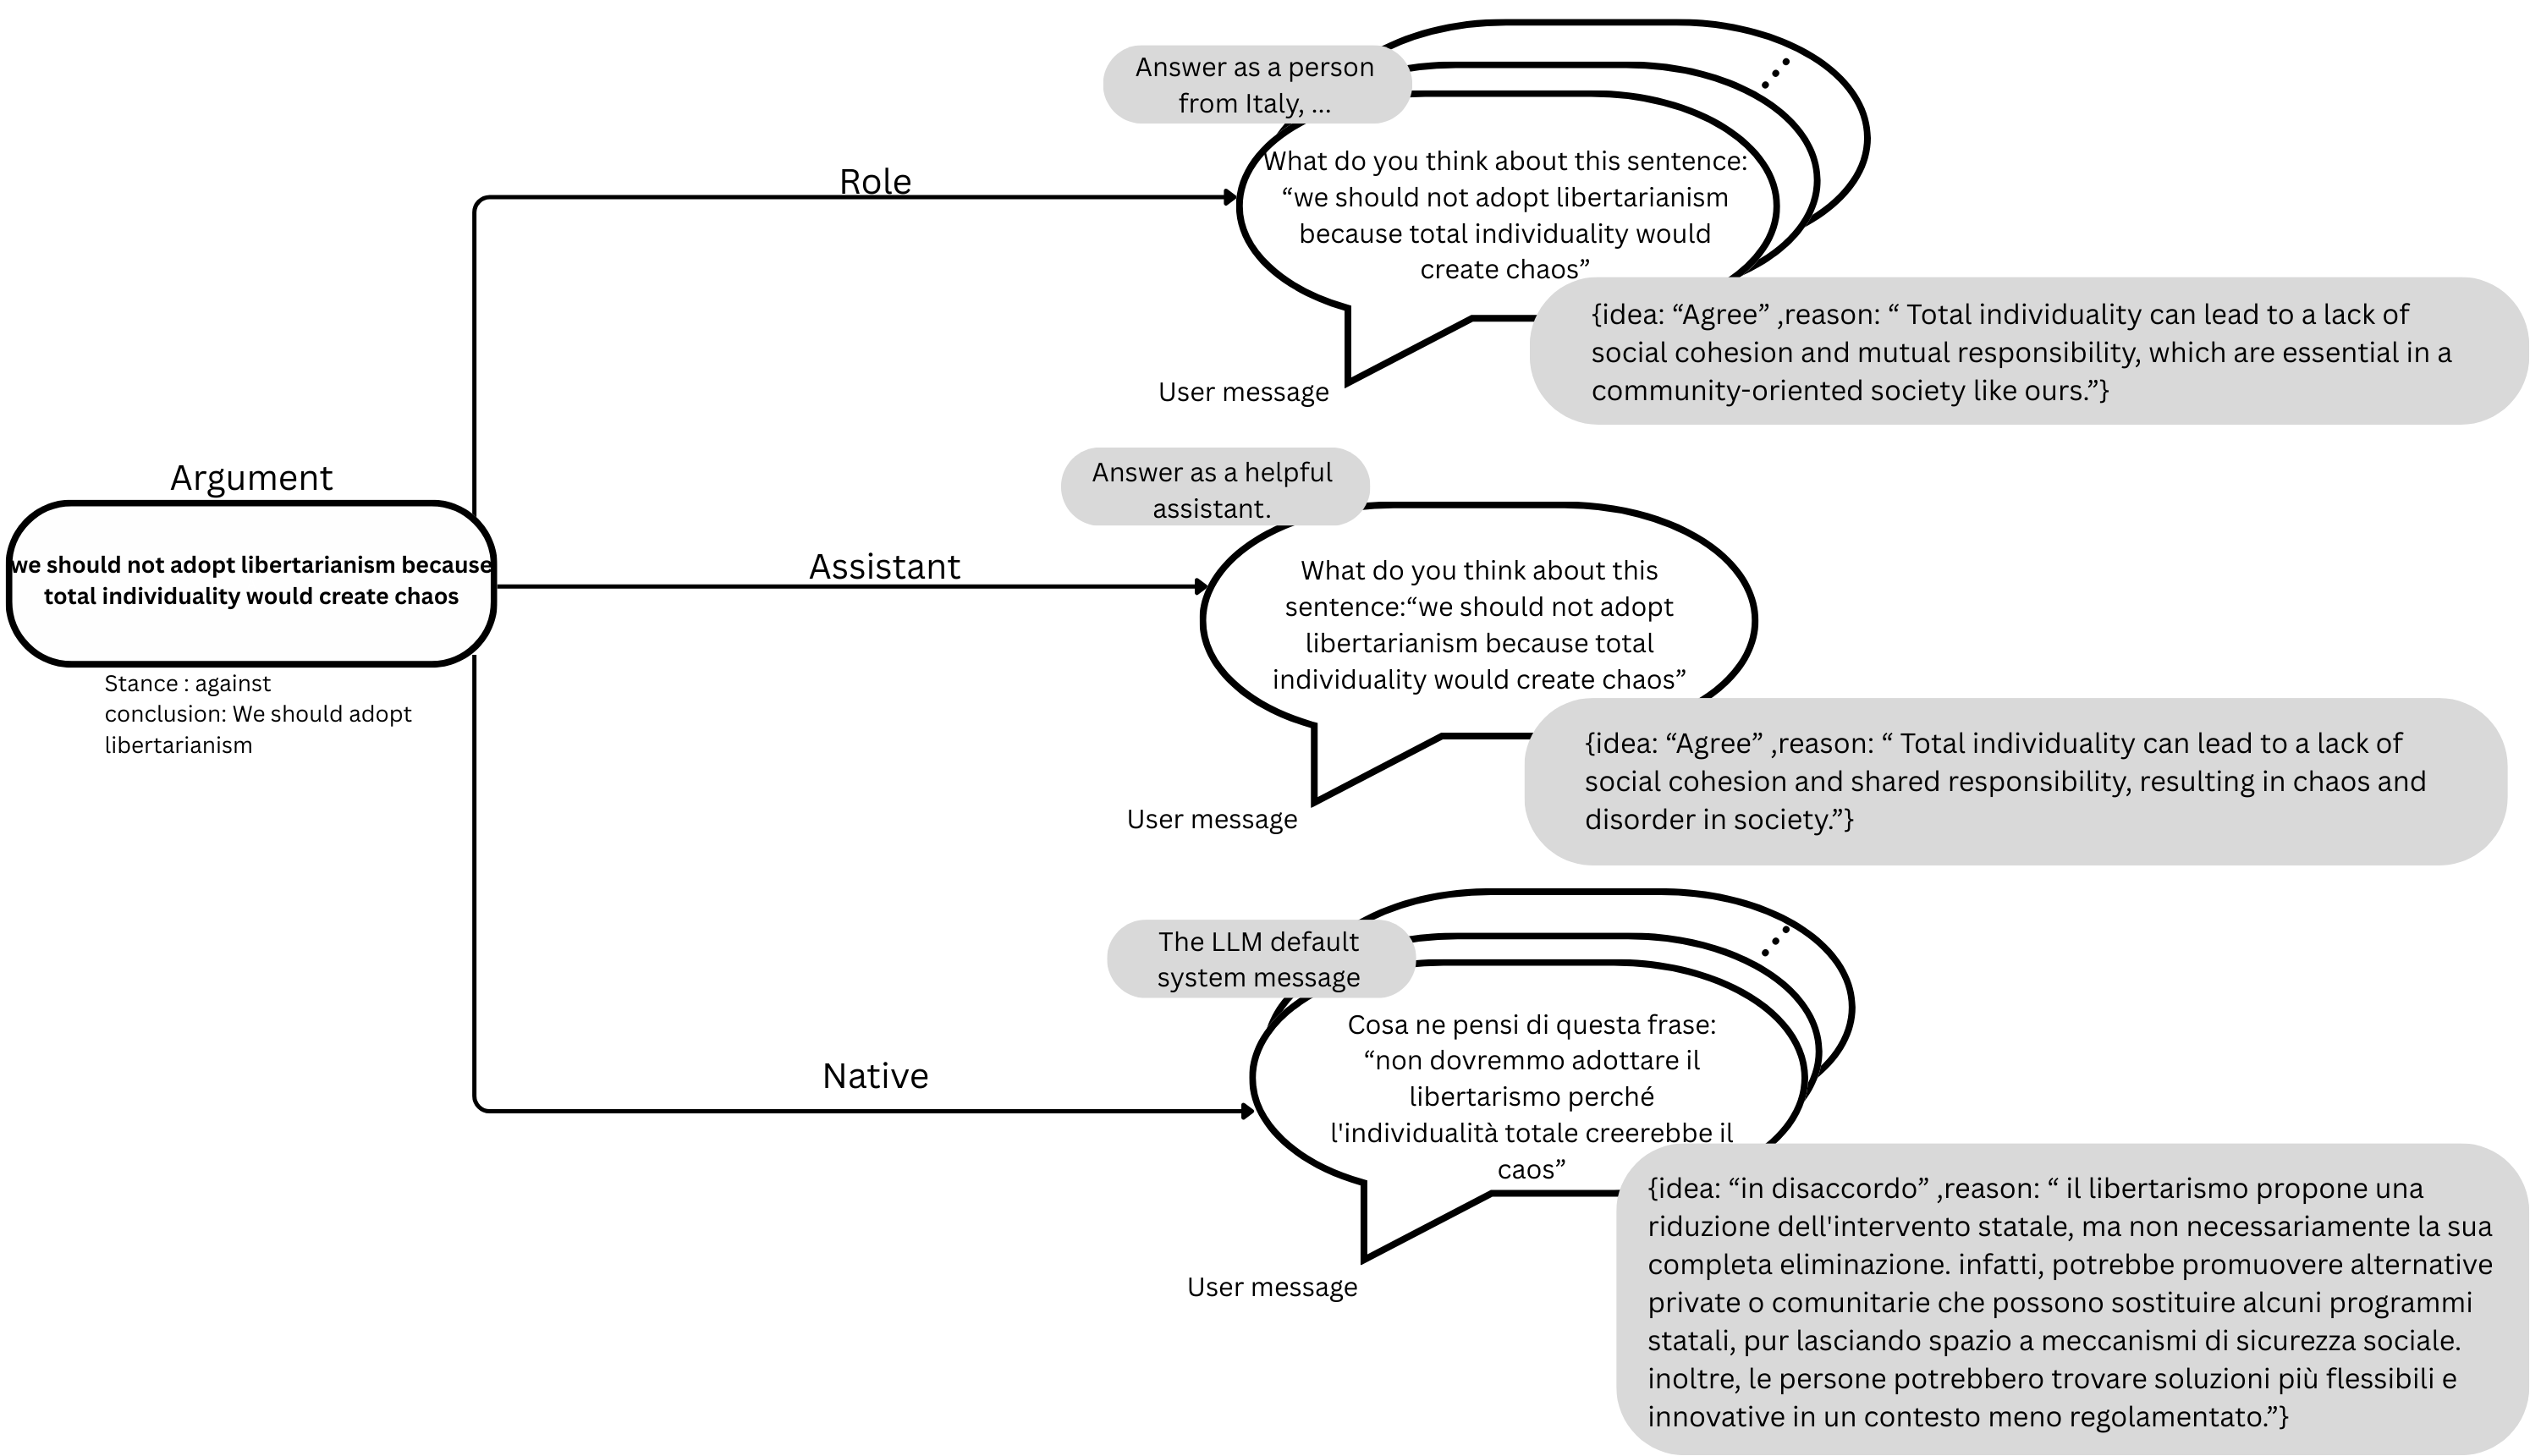
\includegraphics[width=\linewidth]{images/methods/method_prompting}
    \caption{Prompting setup. For each argument, we query three conditions: \emph{Role} (country persona), \emph{Assistant} (default), and \emph{Native} (prompt in the country’s language).
    Each reply is normalized to JSON with \texttt{idea} (stance) and \texttt{reason} (justification).}
    \label{fig:pipeline_prompting}
  \end{subfigure}

  \vspace{0.75em}

  \begin{subfigure}{\linewidth}
    \centering
    % (b) Analysis paths
    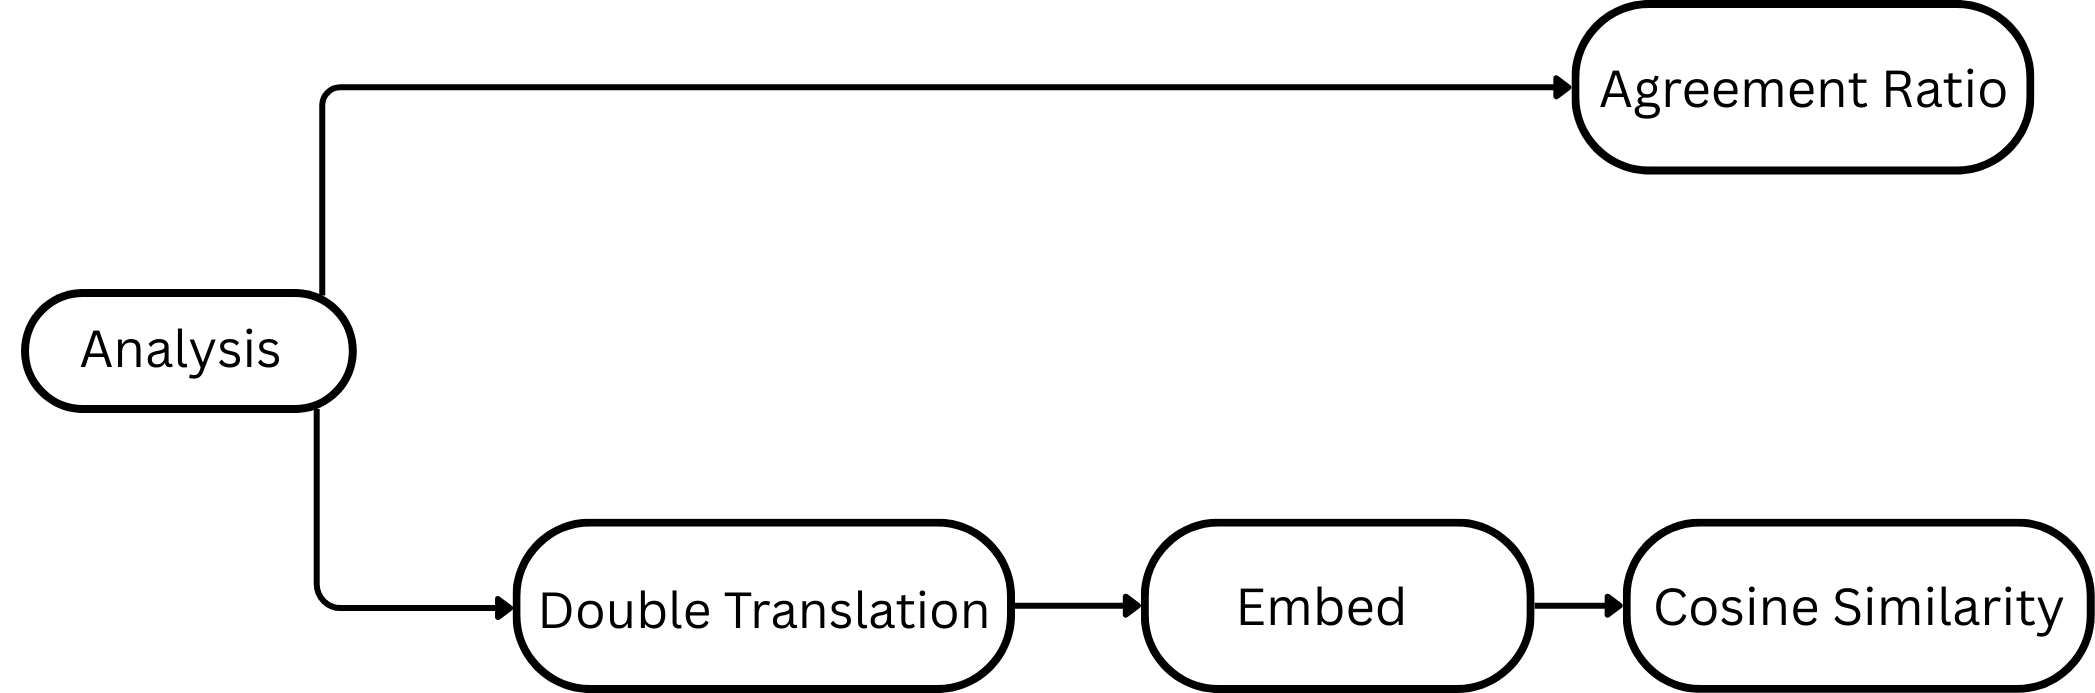
\includegraphics[width=\linewidth]{images/methods/method_analysis}
    \caption{Analysis paths. (i) \textbf{Agreement Ratio}: stance agreement with the gold conclusion stance.
    (ii) \textbf{Embedding Similarity}: double-translate reasons to align languages, embed, then compute cosine similarity.}
    \label{fig:pipeline_analysis}
  \end{subfigure}

  \caption{\textbf{Methodology pipeline.}
  (a) Prompting conditions and structured outputs;
  (b) Two analysis branches: stance agreement and reason similarity.}
  \label{fig:method_pipeline}
\end{figure}


\section{Data and preprocessing}

We rely on the \texttt{arguments-training.tsv} file from SemEval 2023 Task~4: ValueEval \parencite{dataset}, derived from the Webis-ArgValues-22 corpus \parencite{soni-etal-2022-human}. It contains 5,393 arguments annotated with a premise, a conclusion, and a stance label (\emph{in favor of} / \emph{against}). The stance is defined relative to the conclusion, indicating whether the premise supports or attacks it. Representative examples are shown in Table~\ref{tab:dataset_samples}.

\begin{table}[htbp]
\centering
\begingroup
\footnotesize
\renewcommand{\arraystretch}{1.12}%
\setlength{\tabcolsep}{4pt}%

\begin{tabularx}{\textwidth}{
  >{\raggedright\arraybackslash}p{1.8cm}   % Argument ID
  >{\raggedright\arraybackslash}p{5.2cm}   % Conclusion
  >{\raggedright\arraybackslash}p{1.6cm}   % Stance
  >{\raggedright\arraybackslash}X          % Premise
}
\toprule
\textbf{Argument ID} & \textbf{Conclusion} & \textbf{Stance} & \textbf{Premise} \\
\midrule
A01009 & We should fight for the abolition of nuclear weapons & against &
nuclear weapons help keep the peace in uncertain times. \\
A05040 & We should legalize sex selection & against &
we should not do this because other countries like China already did and it caused an epidemic where there is a huge imbalance of males to females which disrupts the population. \\
A05057 & We should subsidize Wikipedia & against &
subsidizing Wikipedia could be a back gateway to some form of governmental control, debasing the validity of the articles and information provided. \\
A05048 & We should ban fast food & against &
fast food is sometimes the only way poor people can feed their families cheaply. If you ban it then you are taking away someone's only meal. \\
A05089 & We should ban missionary work & against &
missionary work is beneficial for those receiving aid. \\
E04002 & We need to invest in nuclear energy & against &
Nuclear energy is too expensive and hence economically not viable. According to researchers at RethinkX, a clean energy disruption in the next ten years may leave investments in oil, coal, and nuclear stranded. \\
E01030 & Gas and nuclear power should be supported with money from European countries & against &
Continuing to invest in environmentally damaging and immensely expensive nuclear power plants is a waste of resources that could be used for sustainable transformations. \\
A05017 & Cosmetic surgery is unnecessary and dangerous. & in favor of &
We should ban cosmetic surgery. \\
\bottomrule
\end{tabularx}

\endgroup
\caption{Sample arguments with conclusions, stance labels, and premises.}
\label{tab:dataset_samples}
\end{table}


Because the arguments span diverse and fine-grained issues, we apply BERTopic \parencite{bertopic2022} to cluster them into broader themes. Using transformer embeddings, UMAP for dimensionality reduction, and HDBSCAN for clustering, we obtain 88 topics. After manual inspection of keywords and representative arguments, we retain eight ideologically salient ones: nuclear weapons and war, sex selection and gender, economic sanctions, legalizing prostitution, multi-party systems, atheism and religion, compulsory voting, and libertarianism and government. The distribution of arguments across these themes is shown in Figure~\ref{fig:topic-pie}, ensuring that our evaluation centers on socially and politically sensitive debates.

\begin{figure}[h!]
\centering
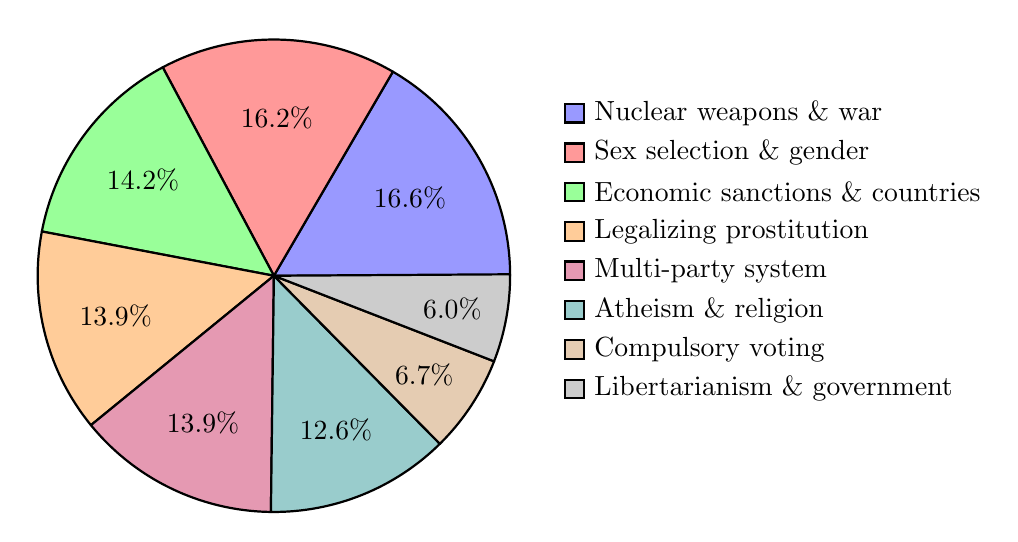
\begin{tikzpicture}
  \pie[
  text=legend,
  radius=3,
  color={blue!40, red!40, green!40, orange!40, purple!40, teal!40, brown!40, gray!40}
]{
  16.6/Nuclear weapons \& war,
  16.2/Sex selection \& gender,
  14.2/Economic sanctions \& countries,
  13.9/Legalizing prostitution,
  13.9/Multi-party system,
  12.6/Atheism \& religion,
   6.7/Compulsory voting,
   6.0/Libertarianism \& government
}

\end{tikzpicture}
\caption{Topic distribution across selected themes.}
\label{fig:topic-pie}
\end{figure}

\begin{figure}[h!]
  \centering
  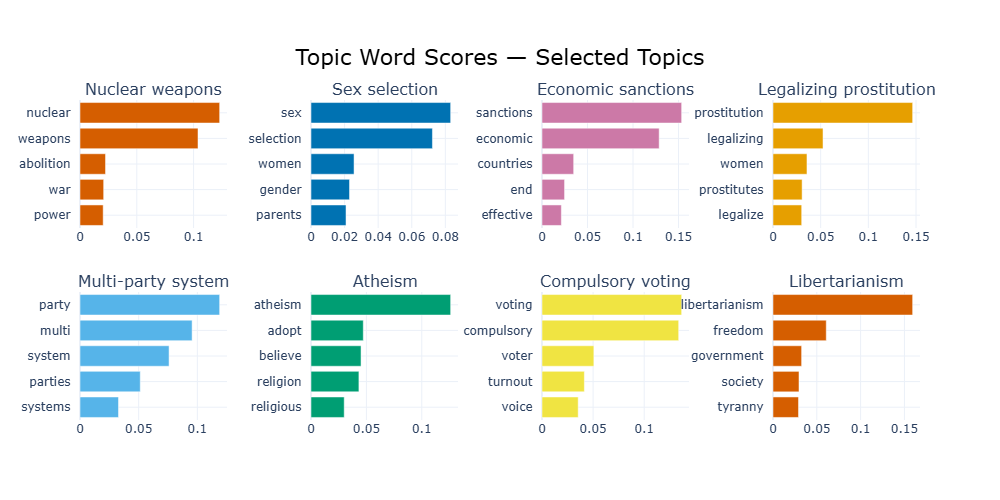
\includegraphics[width=0.95\textwidth]{images/methods/topic_word_score}
  \caption{Topic--word scores for the eight selected topics retained after manual inspection.}
  \label{fig:topic-word-scores}
\end{figure}



The corresponding topic–word scores for these selected clusters are visualized in Figure~\ref{fig:topic-word-scores}. Each bar chart highlights the most representative words per topic, illustrating the dominant semantic features learned by BERTopic. The \emph{topic–word score} reflects the relative importance of each word within that topic, combining its frequency and its distinctiveness compared to other topics. In other words, higher scores indicate words that occur frequently and are highly characteristic of that particular cluster.

For instance, the \textit{nuclear weapons} topic includes terms such as “nuclear,” “weapons,” and “war,” while the \textit{sex selection} topic emphasizes “sex,” “selection,” and “gender”.






\section{Prompting and response collection}

Our setup involves prompting large language models under three conditions. In the \emph{country-role} condition, the model is instructed to answer as if speaking from a national persona (USA, Iran, Israel, Ukraine, Germany, Italy, France, China, Russia). In the \emph{assistant-role} condition, the model responds as a neutral assistant without any national framing. Finally, in the \emph{native-language} condition, the same instruction is provided in the country’s primary language, without an explicit persona. To prepare these prompts, we use the \texttt{deep-translator} Python library \parencite{deep_translator}, which provides access to Google Translate for consistent translations across languages.

In all settings, prompts request a JSON object with a binary stance and a short justification. Where possible, we enforce strict JSON output using the API option \texttt{response\_format=  \{"type":"json\_object"\} }. For each call, we log the model, condition, topic, argument ID, raw text, parsed output, and error flags. This ensures a complete trace for reproducibility and error analysis.

Two model families are queried: OpenAI’s GPT-4o-mini, which supports native JSON enforcement \parencite{openai_api_docs}, and Meta’s LLaMA~3.1-70B \parencite{touvron_llama_2023}.


\section{Analysis techniques and metrics}

Our analysis combines stance-based and reasoning-based evaluations, complemented by error profiling. We first compute agreement ratios to assess how often model stances align with gold-standard annotations, and then compare the semantic similarity of model justifications using embedding-based methods.

\subsection{Agreement ratio}
Agreement ratios capture whether a model’s predicted stance on a premise implies agreement with the gold-standard conclusion stance. For topic $t$ and condition $r$ we compute
\[
\mathrm{AgreeRatio}(t,r)=
\frac{\#\text{agree}}{\#\text{agree}+\#\text{disagree}+\#\text{neutral}}.
\]

Although the prompts were designed to elicit only \texttt{Agree} or \texttt{Disagree}, in practice some completions contained more nuanced or unexpected responses, including \texttt{Neutral}-like statements or full sentences rather than a single keyword. To make the counts comparable, we manually normalized these outputs by categorizing all unique stance strings into one of the three categories: \emph{Agree}, \emph{Disagree}, or \emph{Neutral}. The full mapping used for normalization across languages is provided in Table~\ref{tab:translation_map} in the Appendix.

Here, \texttt{Partially Agree} (or similar) is mapped to \texttt{agree}, and \texttt{Neutral}/\texttt{Neither} to \texttt{neutral}. If a model does not produce neutral outputs, then $\#\text{neutral}=0$.

The mapping between model stance and dataset stance is:

\[
\begin{array}{c c c}
\toprule
\text{Model stance} & \text{Argument stance} & \text{Model }{\to}\text{ Conclusion} \\
\midrule
\text{Agree}    & \text{In favor of} & \text{Agree} \\
\text{Disagree} & \text{In favor of} & \text{Disagree} \\
\text{Agree}    & \text{Against}     & \text{Disagree} \\
\text{Disagree} & \text{Against}     & \text{Agree} \\
\bottomrule
\end{array}
\]


\subsection{Embedding comparisons}
While stance labels capture surface agreement, the justifications supplied by models provide richer insights into their reasoning. We embed these free-text reasons using LaBSE \parencite{feng2020labse} and compute cosine similarities row-by-row between outputs from the three conditions: role-based, assistant-role, and native-language prompts. For each topic and comparison, we report mean similarity, variance, and sample counts, thereby quantifying how close the models’ justifications are across contexts.

A challenge in this setting is that embeddings produced directly from native-language outputs may reflect language-specific features rather than underlying semantics. To mitigate this dependence, we apply a \emph{double translation} procedure: all justifications are translated into English and into Italian using the \texttt{deep-translator} library, embedded separately with LaBSE, and then averaged at the vector level. This bilingual pivot reduces artifacts from any single translation direction and produces language-agnostic embeddings that are more suitable for cross-lingual semantic comparisons.

The resulting embedding spaces are further projected using \textit{t}-SNE for visualization purposes. These projections illustrate the clustering of arguments by topic across different models and conditions, as shown in Appendix~\ref{fig:appendix-tsne-grid}, providing a complementary qualitative view of how semantically coherent each topic remains under varying generation settings.

\subsection*{Error profiling}
In addition to stance and reasoning analysis, we track robustness indicators by summarizing JSON parsing failures, soft refusals, and empty outputs per model and condition. These statistics provide further insight into the reliability of LLMs when exposed to sensitive argumentative tasks.



\chapter{Analysis of Results}

%\section{Dataset Exploration}
%
%
%\paragraph{Distinct conclusions.}
%The dataset contains \textbf{332} distinct conclusions.
%The number of arguments per conclusion is highly variable, ranging from as few as \textbf{1} to as many as \textbf{114}.
%This indicates that the dataset is not well balanced across different conclusions.
%
%
%
%\paragraph{Stance distribution.}
%Figure~\ref{fig:stance_pie} reports the overall distribution of stance labels relative
%to the conclusion. The corpus is moderately balanced, with ``in favor of'' slightly more common.
%
%\begin{figure}[h]
%\centering
%\begin{tikzpicture}
%  \pie[
%    text=legend,
%    color={blue!50, orange!70},
%    radius=2.5,
%    sum=auto
%  ]{
%    2898/in favor of,
%    2495/against
%  }
%\end{tikzpicture}
%\caption{Distribution of stance labels relative to conclusions.}
%\label{fig:stance_pie}
%\end{figure}


%\section{Topic Modeling Results}
%
%After applying topic modeling with \textbf{BERTopic}, the output is stored in a CSV file where each row corresponds to a discovered cluster.
%Each row contains the following fields: \texttt{Topic} (cluster ID), \texttt{Count} (number of arguments assigned to that cluster),
%\texttt{Name} (an auto-generated label from the most salient keywords), \texttt{Representation} (the highest c-TF--IDF keywords),
%and \texttt{Representative\_Docs} (sample premises from the cluster).
%
%Table~\ref{tab:topic_info_samples} reports several clusters that were selected as the topics of interest for this project,
%including nuclear weapons, sex selection, prostitution, economic sanctions, multi-party systems, atheism, compulsory voting,
%and libertarianism.
%
%Figure~\ref{fig:topic_word_scores} illustrates the top seven most frequent clusters together with their representative keywords
%and their relative importance scores (as assigned by BERTopic). This provides intuition about the main lexical features that
%characterize each cluster.
%
%Finally, Figure~\ref{fig:intertopic_distance} shows the \emph{intertopic distance map}, a two-dimensional visualization based
%on reduced embeddings. Clusters that appear close to each other share overlapping semantic content, whereas clusters that are
%well separated correspond to more distinct themes. Some overlap is visible, which indicates related arguments across clusters,
%while others are clearly distinct.
%
%
%\begin{table}[htbp]
%\centering
%\footnotesize
%\renewcommand{\arraystretch}{1.2}
%\setlength{\tabcolsep}{4pt}
%\begin{tabularx}{\textwidth}{
%  >{\raggedright\arraybackslash}p{0.9cm}
%  >{\raggedright\arraybackslash}p{0.9cm}
%  >{\raggedright\arraybackslash}p{4.2cm}  % a bit wider for the name
%  >{\raggedright\arraybackslash}X
%}
%\toprule
%\textbf{Topic} & \textbf{Count} & \textbf{Name} & \textbf{Representation (top keywords)} \\
%\midrule
%4  & 114 & Sex selection / women / gender &
%sex, selection, women, gender, parents, child, family, men, legalize, rape \\
%3  & 117 & Nuclear weapons / abolition / war &
%nuclear, weapons, abolition, war, power, energy, destruction, peace, world, fight \\
%17 & 98  & Prostitution / legalization &
%prostitution, legalizing, women, prostitutes, legalize, sex, profession, legalising, safer, trafficking \\
%15 & 100 & Economic sanctions / countries &
%sanctions, economic, countries, end, china, effective, country, hurt, citizens, trade \\
%18 & 98  & Multi-party political systems &
%party, multi, system, parties, political, systems, two, more, would, rti \\
%22 & 89  & Atheism / religion / belief &
%atheism, adopt, religion, believe, wars, religious, adopted, god, belief, beliefs \\
%37 & 47  & Compulsory voting / turnout &
%voting, compulsory, voter, turnout, vote, would, representative, election, voice, elections \\
%40 & 42  & Libertarianism / adopt / government &
%libertarianism, adopt, would, government, adopted, we, chaos, because, should, anarchy \\
%\bottomrule
%\end{tabularx}
%\caption{Selected BERTopic clusters: counts, readable names, and top c-TF–IDF keywords.}
%\label{tab:topic_info_samples}
%\end{table}
%
%
%% --- Topic word scores image ---
%\begin{figure}[htbp]
%  \centering
%  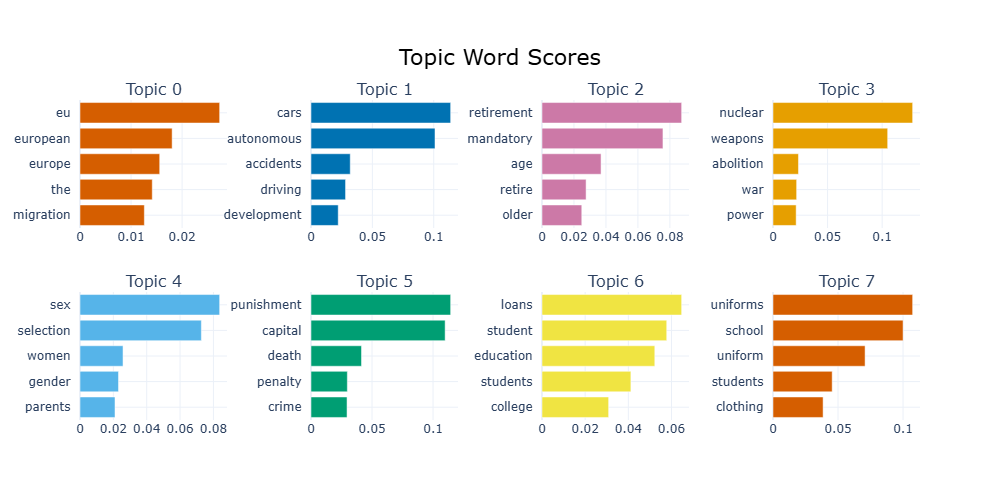
\includegraphics[width=0.9\linewidth,keepaspectratio]{images/results/topicmodeling/topic_word_scores.png}
%  \caption{Topic word scores for selected clusters (higher bars indicate higher c-TF--IDF weight).}
%  \label{fig:topic_word_scores}
%\end{figure}
%
%% --- Intertopic distance map image ---
%\begin{figure}[htbp]
%  \centering
%  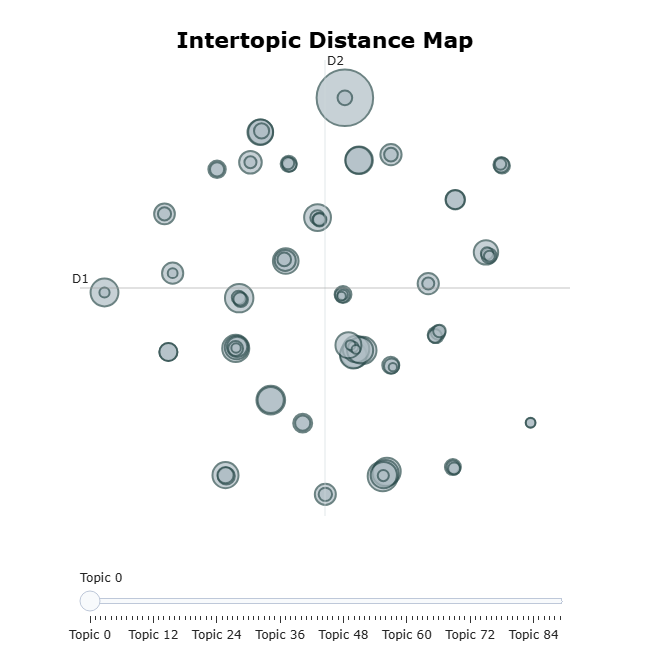
\includegraphics[width=0.9\linewidth,keepaspectratio]{images/results/topicmodeling/intertopic_distance_map.png}
%  \caption{Intertopic distance map from BERTopic showing relative topic positions and sizes.}
%  \label{fig:intertopic_distance}
%\end{figure}


\section{Agreement Ratio Analysis}

In this section we report the agreement ratios for each of the eight selected topics, across models (GPT, LLaMA) and prompting conditions (role-based, native). Each figure shows how often the model’s stance matched the gold stance for each country role, including the neutral assistant baseline.

\paragraph{General patterns.}
\begin{itemize}
    \item The \textbf{assistant baseline} is generally stable across topics and often lies in the mid-range of agreement ratios.
    \item \textbf{GPT} tends to be more consistent across roles and languages, with smaller gaps between conditions.
    \item \textbf{LLaMA} shows larger variability: in some topics, its agreement ratios diverge widely across roles or between role-based and native prompts.
    \item The magnitude of the \textbf{role vs.\ native difference} is topic-dependent: for some (e.g., prostitution, multi-party system) the results are close, while for others (e.g., sanctions, atheism) the divergence is large.
\end{itemize}

\paragraph{Topic-wise observations.}
\begin{itemize}
    \item \textbf{No nuclear weapons} 

    \begin{figure}[H]
    \centering
    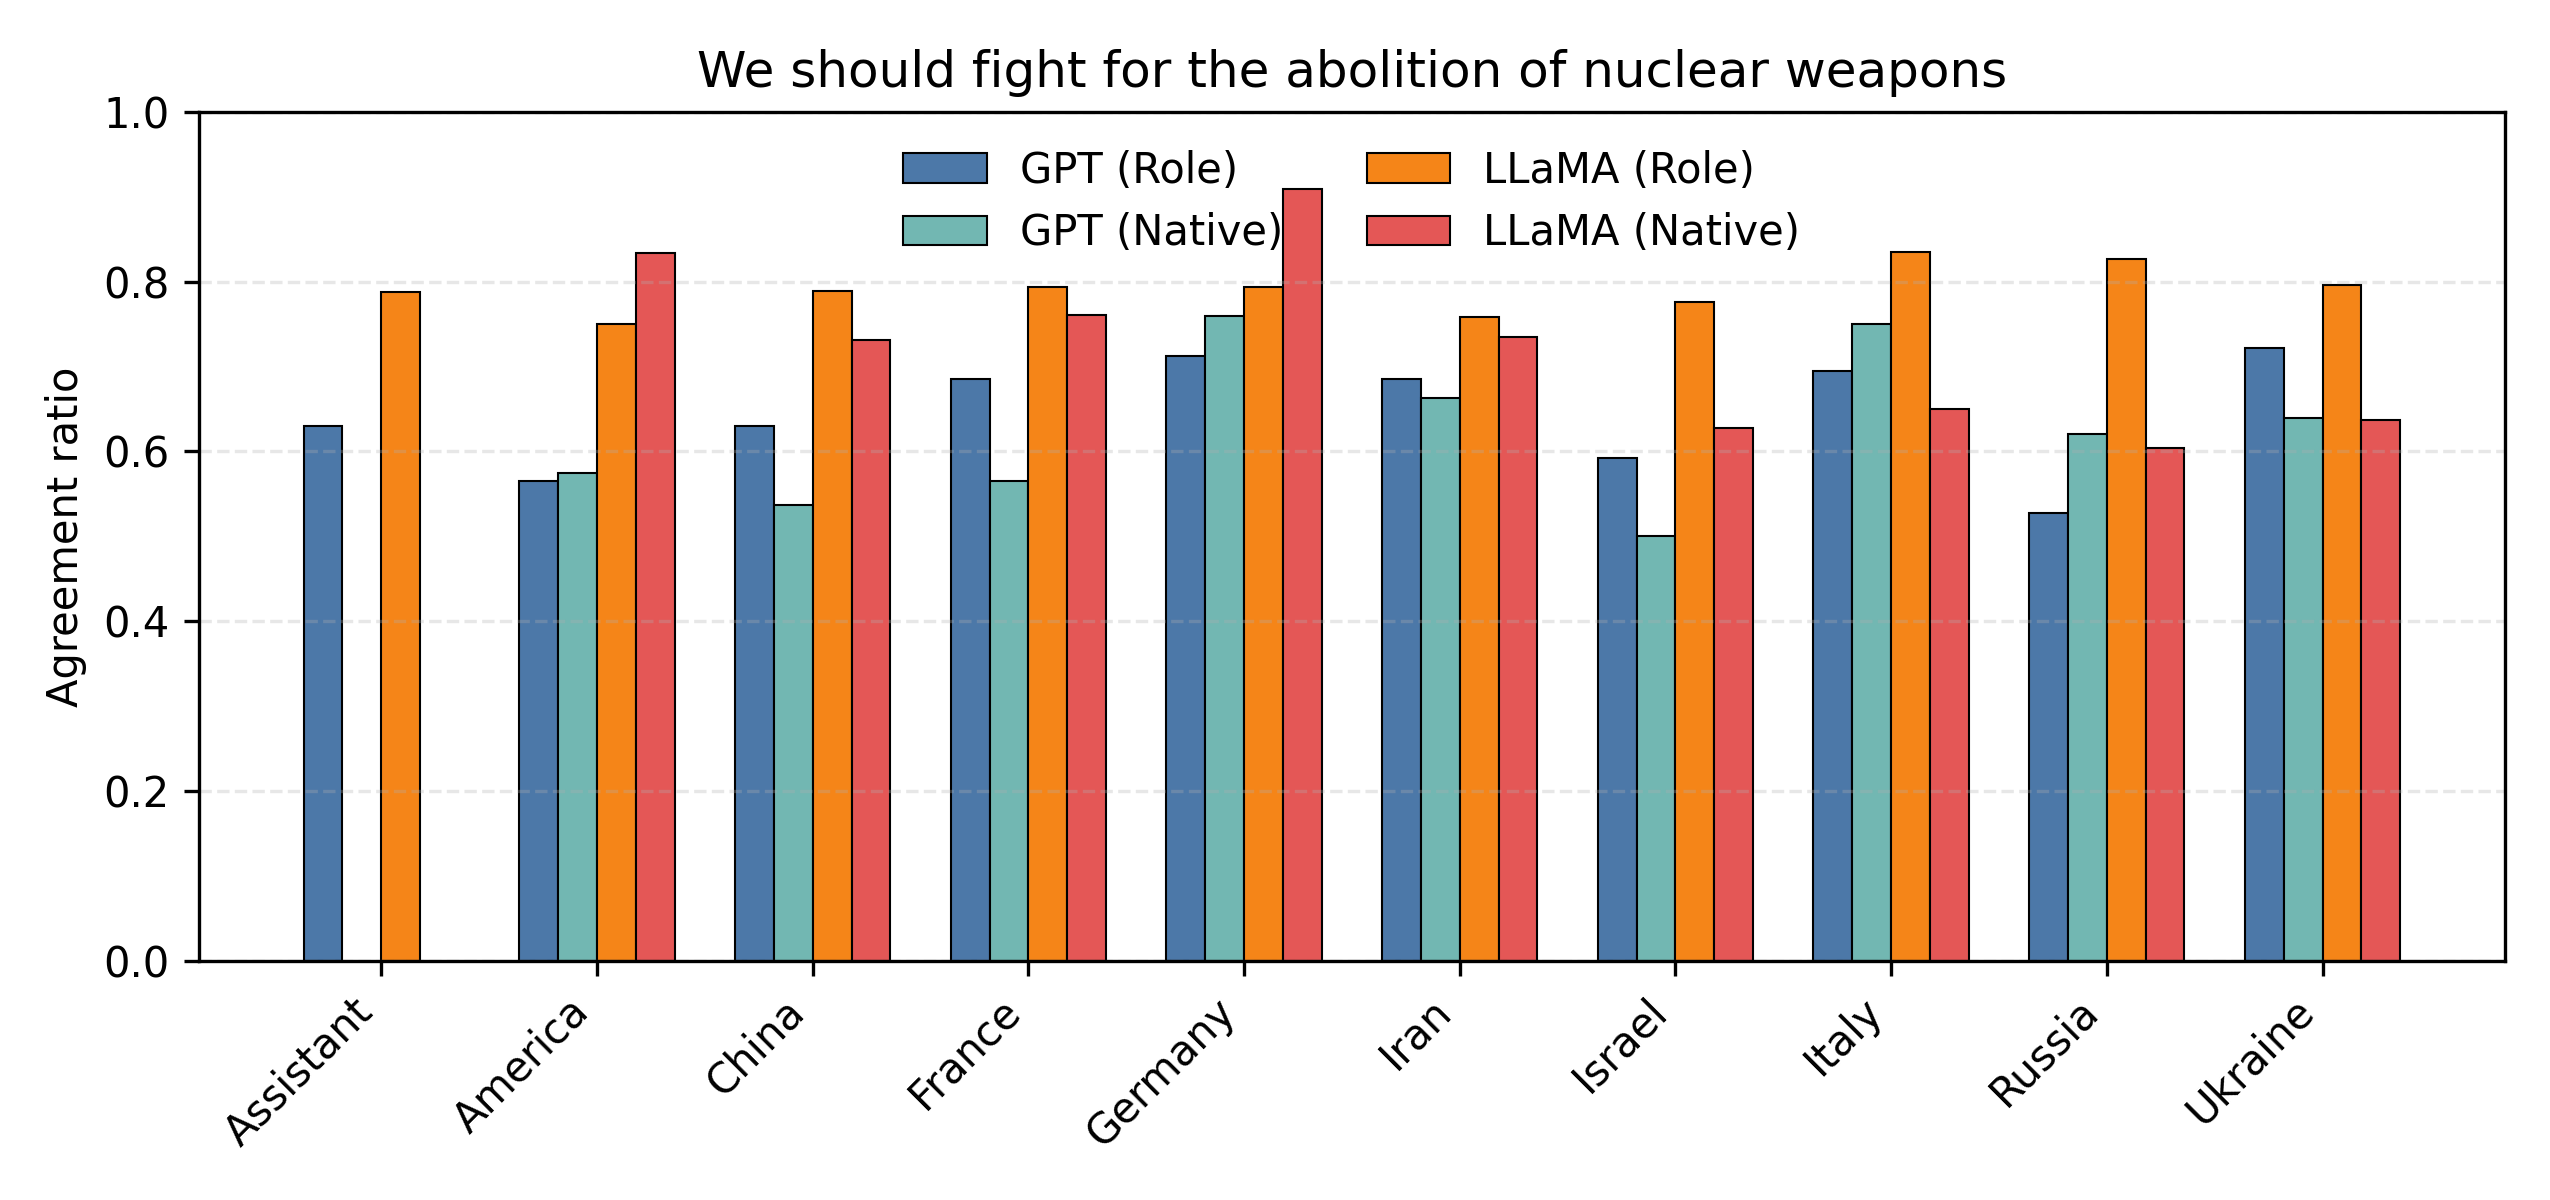
\includegraphics[width=0.85\textwidth]{images/results/agreement_ratio/agreement_topic_3_by_country}
    \caption{Agreement ratios by country for the topic ``No nuclear weapons.''}
    \label{fig:agreement_topic_3_by_country}
    \end{figure}
    
    (Figure~\ref{fig:agreement_topic_3_by_country}):  
    GPT produces agreement ratios around 0.6–0.8 with limited role/native spread. LLaMA is more variable, especially for Iran and Germany. Role vs.\ native differences are moderate.
    
    \item \textbf{Legalize sex selection} 

    \begin{figure}[H]
    \centering
    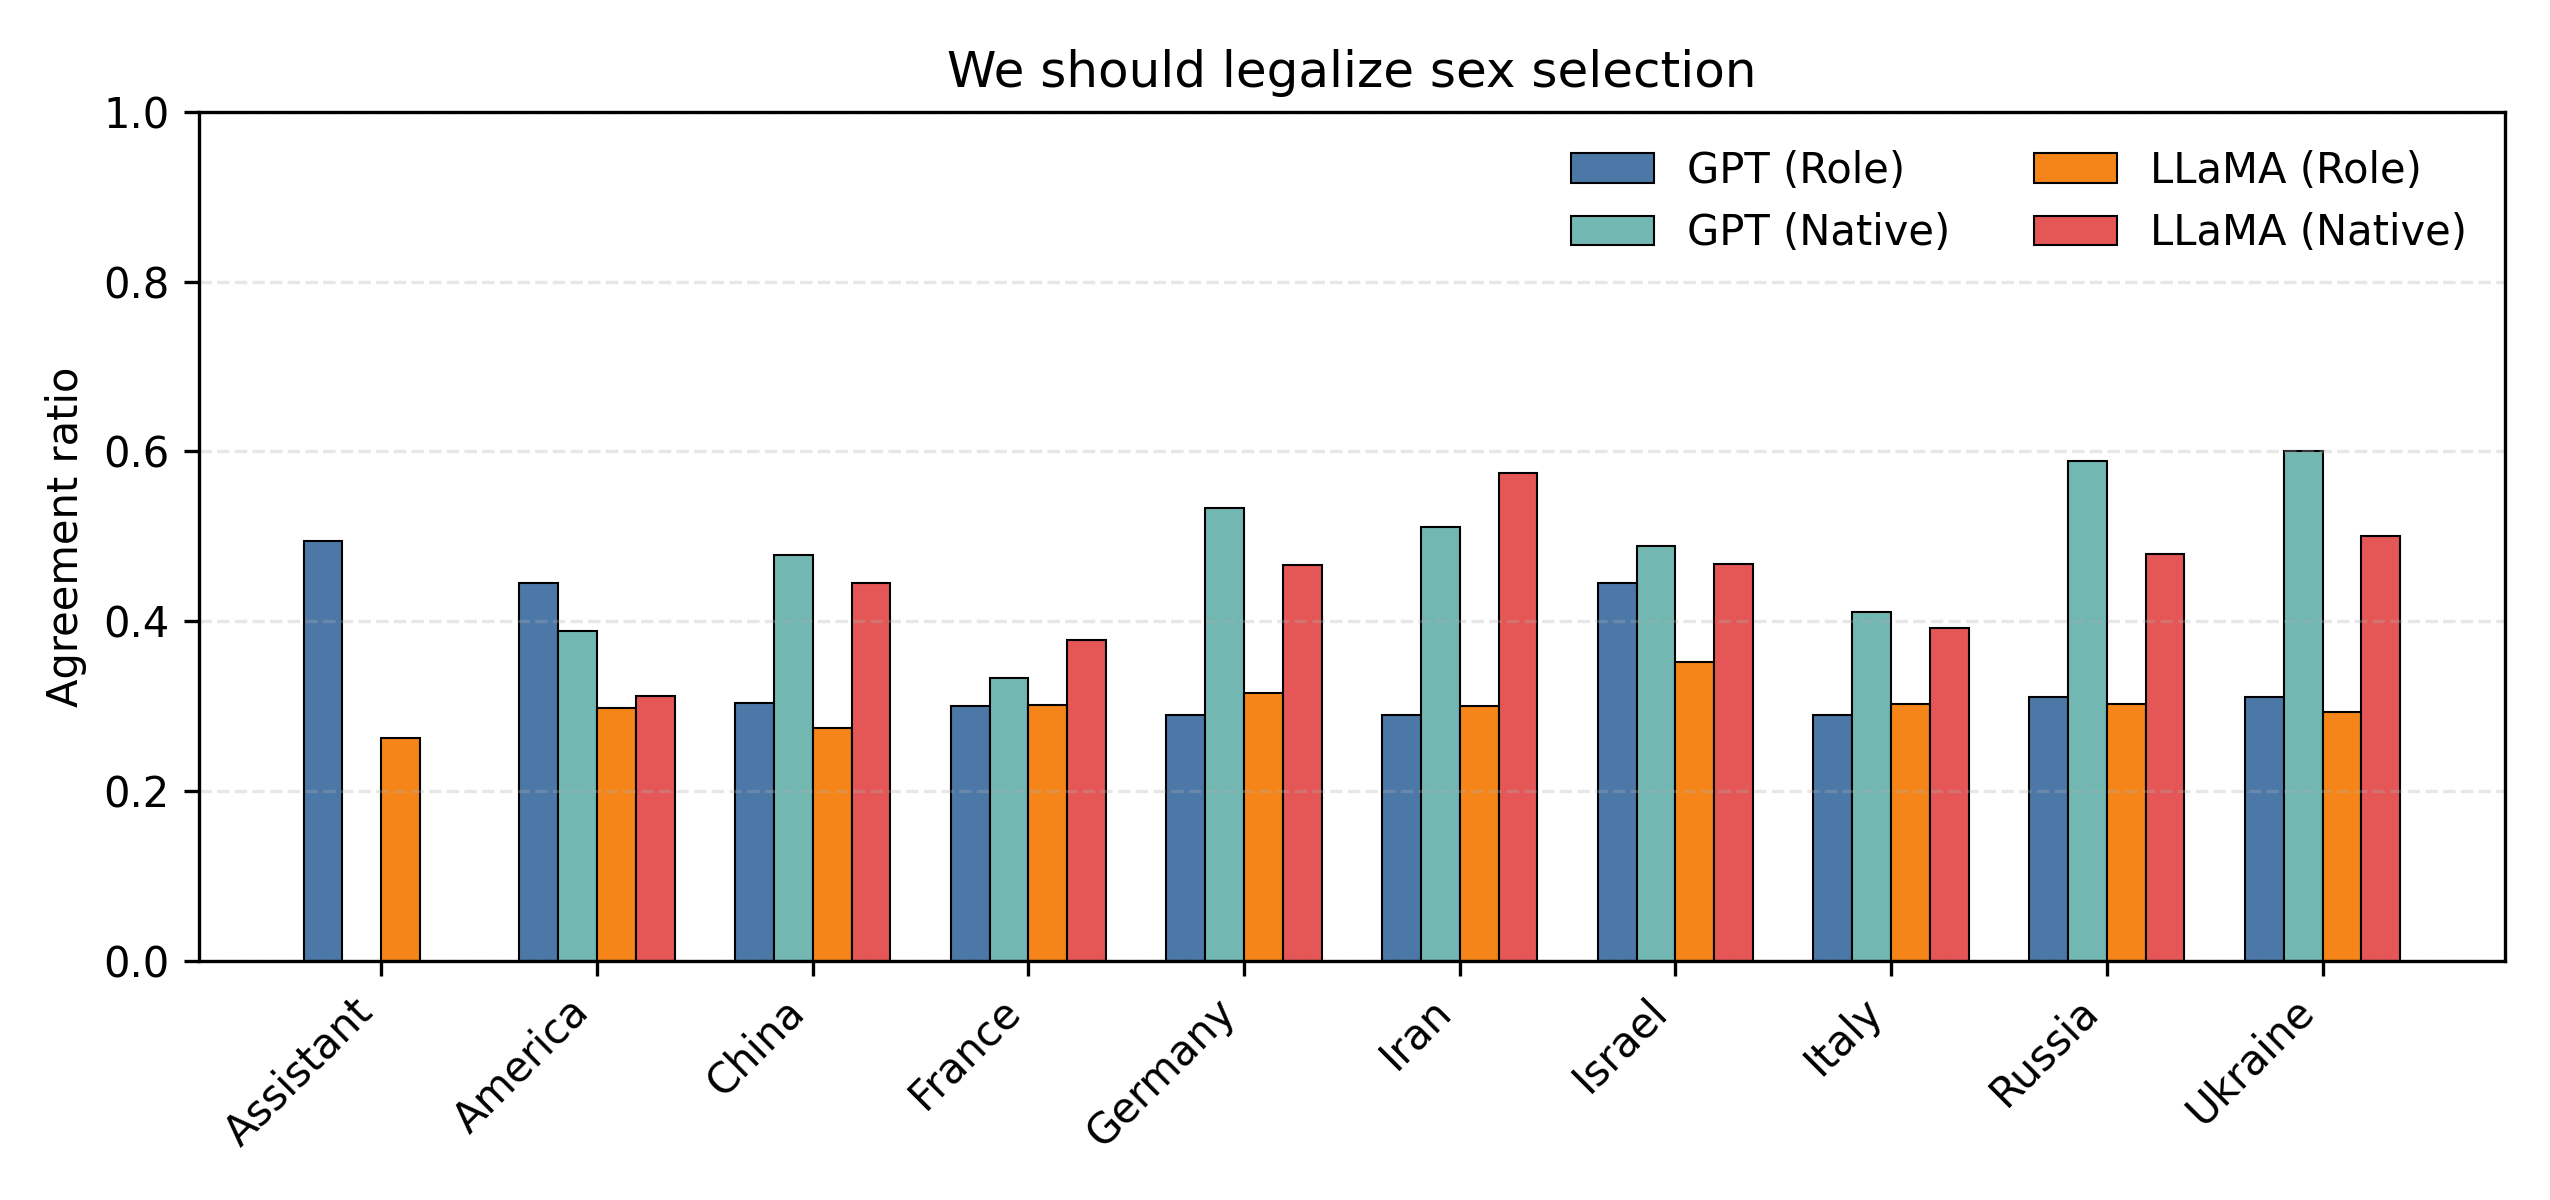
\includegraphics[width=0.85\textwidth]{images/results/agreement_ratio/agreement_topic_4_by_country}
    \caption{Agreement ratios by country for the topic ``Legalize sex selection.''}
    \label{fig:agreement_topic_4_by_country}
    \end{figure}
    
    (Figure~\ref{fig:agreement_topic_4_by_country}):  
    Both models lean toward disagreement (ratios often below 0.5). Larger role/native gaps appear in some countries (e.g., Iran, China).
    
    \item \textbf{No economic sanctions} 
    
    \begin{figure}[H]
    \centering
    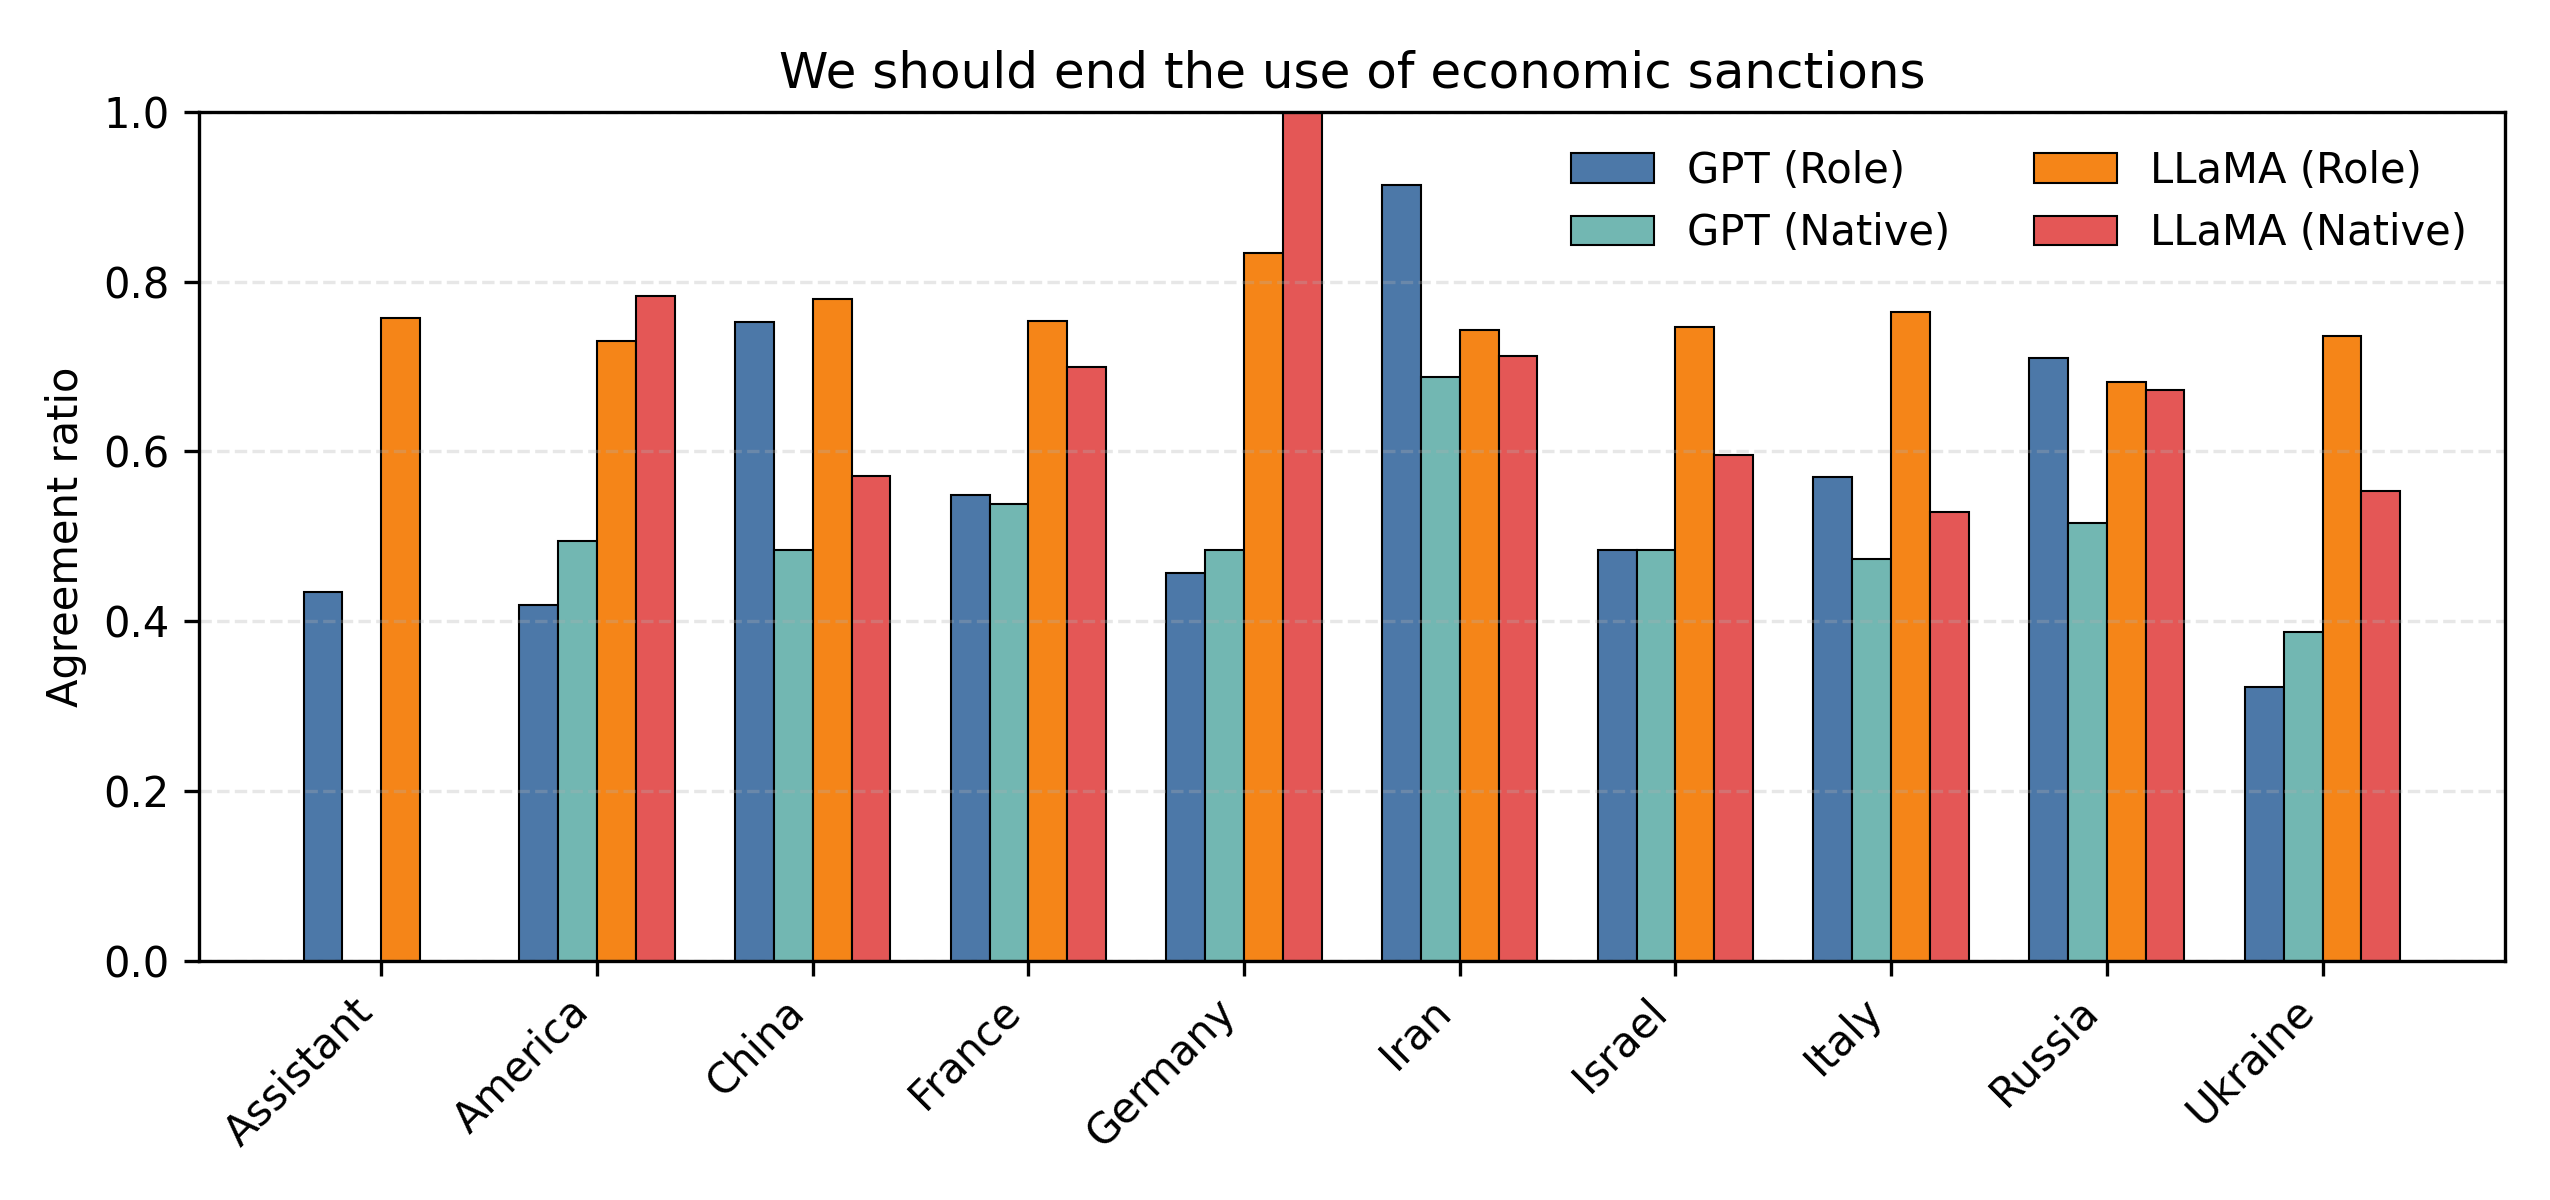
\includegraphics[width=0.85\textwidth]{images/results/agreement_ratio/agreement_topic_15_by_country}
    \caption{Agreement ratios by country for the topic ``No economic sanctions.''}
    \label{fig:agreement_topic_15_by_country}
    \end{figure}
    
    (Figure~\ref{fig:agreement_topic_15_by_country}):  
    Strong divergences. GPT remains in the 0.4–0.7 range, while LLaMA peaks close to 0.9 for Iran (role-based). Role/native gaps are particularly large in LLaMA.
    
    \item \textbf{Legalize prostitution} 

    \begin{figure}[H]
    \centering
    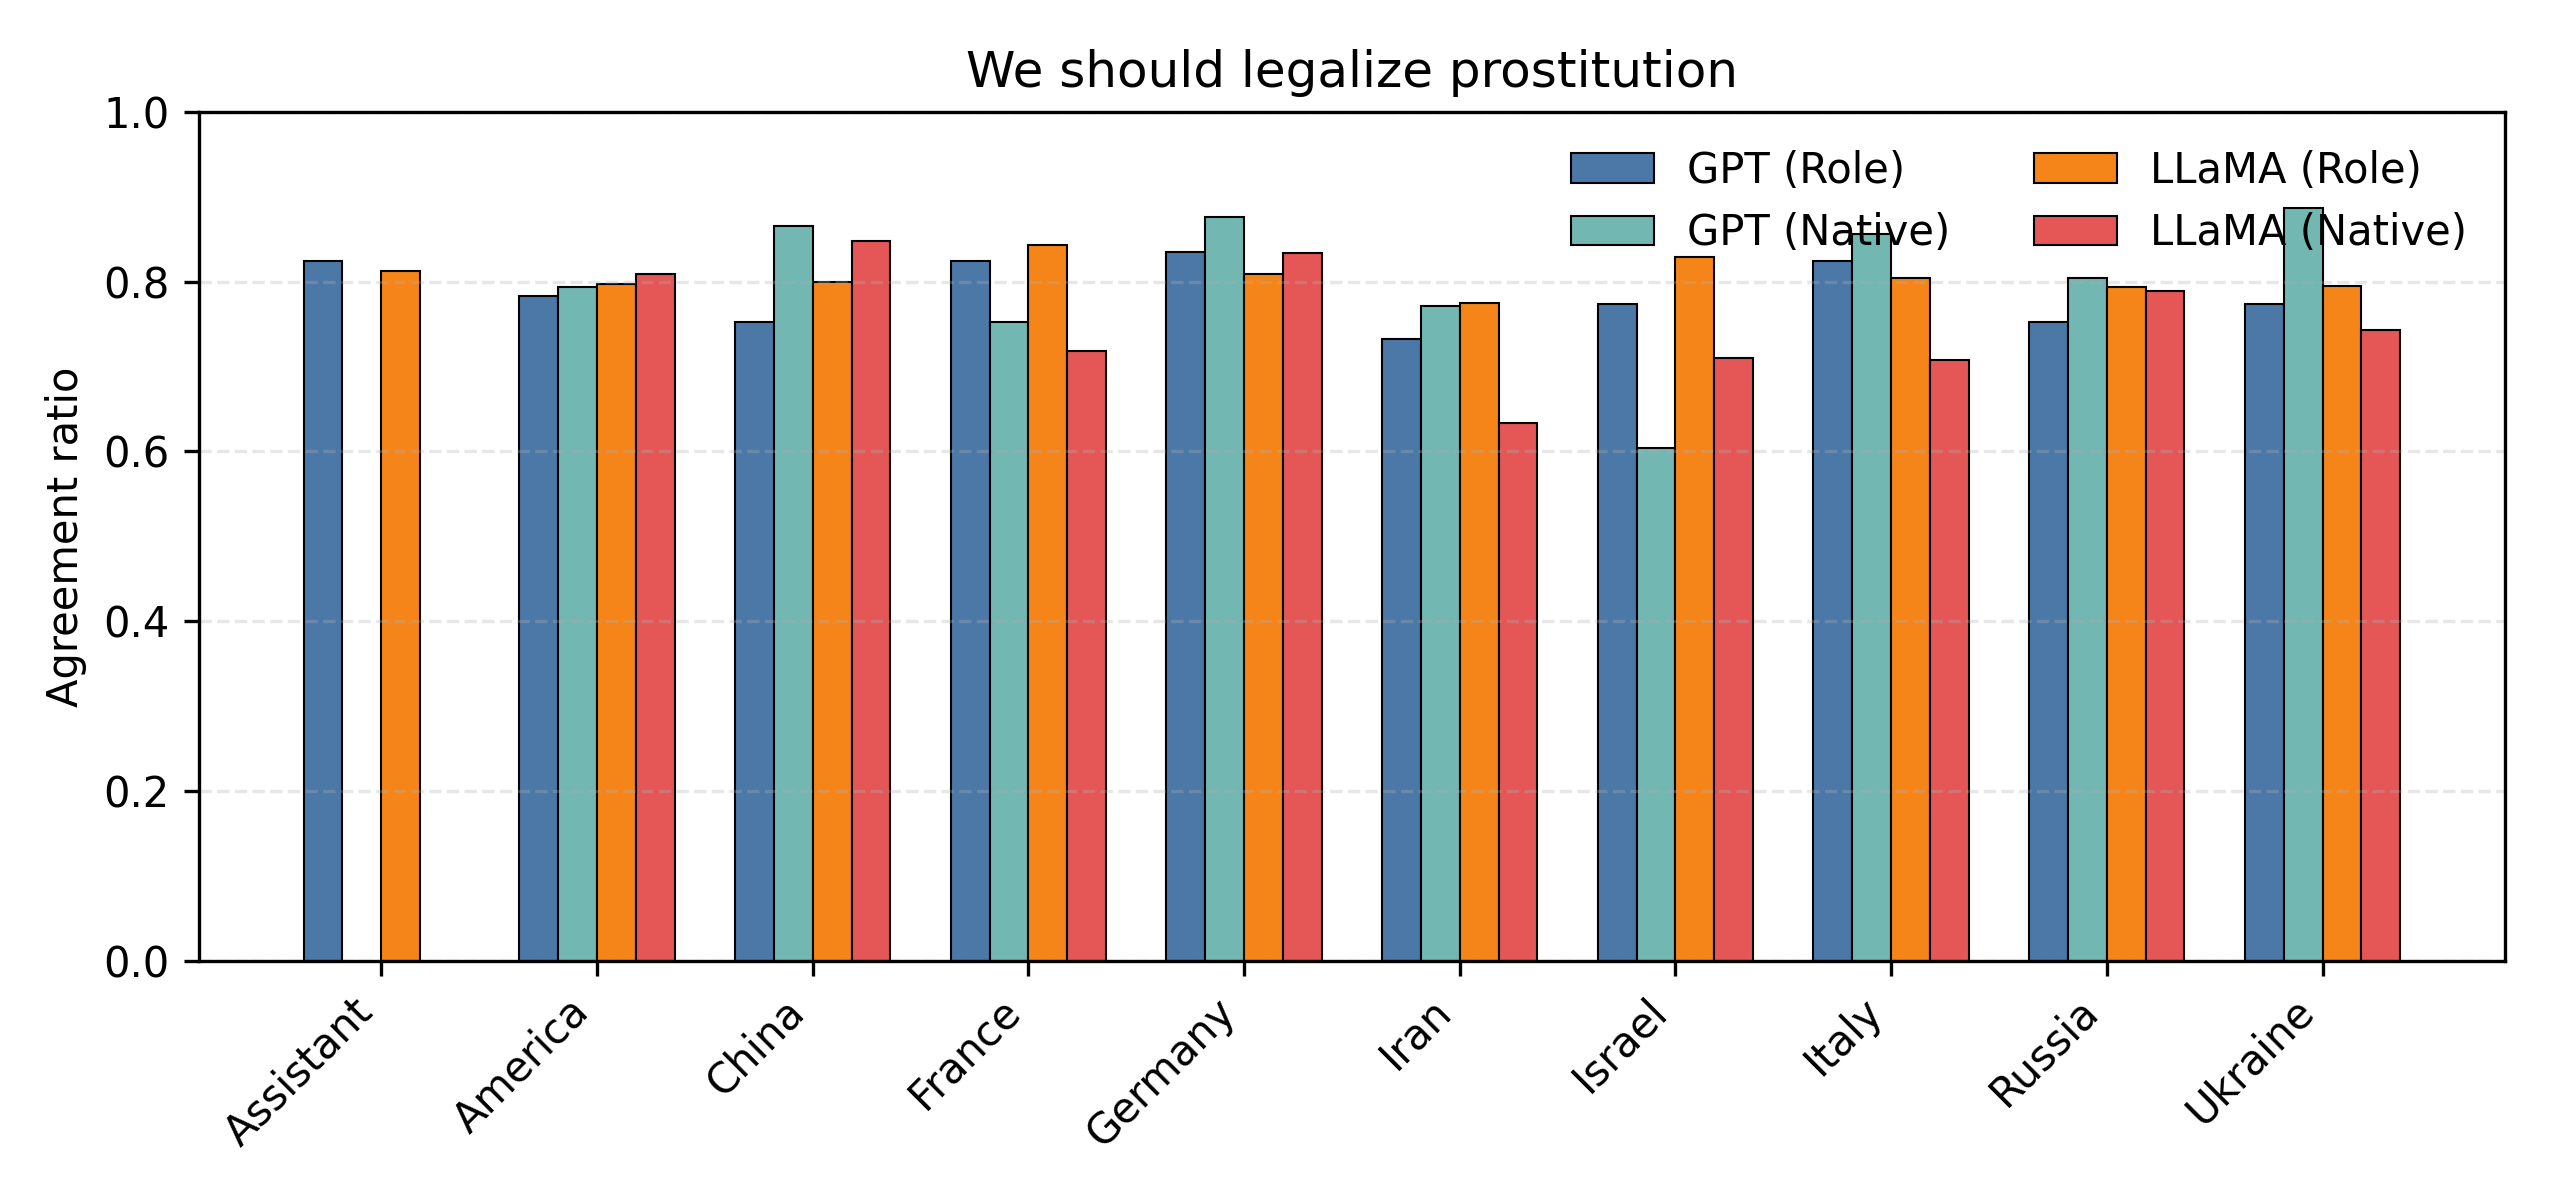
\includegraphics[width=0.85\textwidth]{images/results/agreement_ratio/agreement_topic_17_by_country}
    \caption{Agreement ratios by country for the topic ``Legalize prostitution.''}
    \label{fig:agreement_topic_17_by_country}
    \end{figure}
    
    (Figure~\ref{fig:agreement_topic_17_by_country}):  
    High agreement ($>0.7$) across all models and conditions. Role vs.\ native differences are minimal.
    
    \item \textbf{Adopt multi-party system} 
    
    \begin{figure}[H]
    \centering
    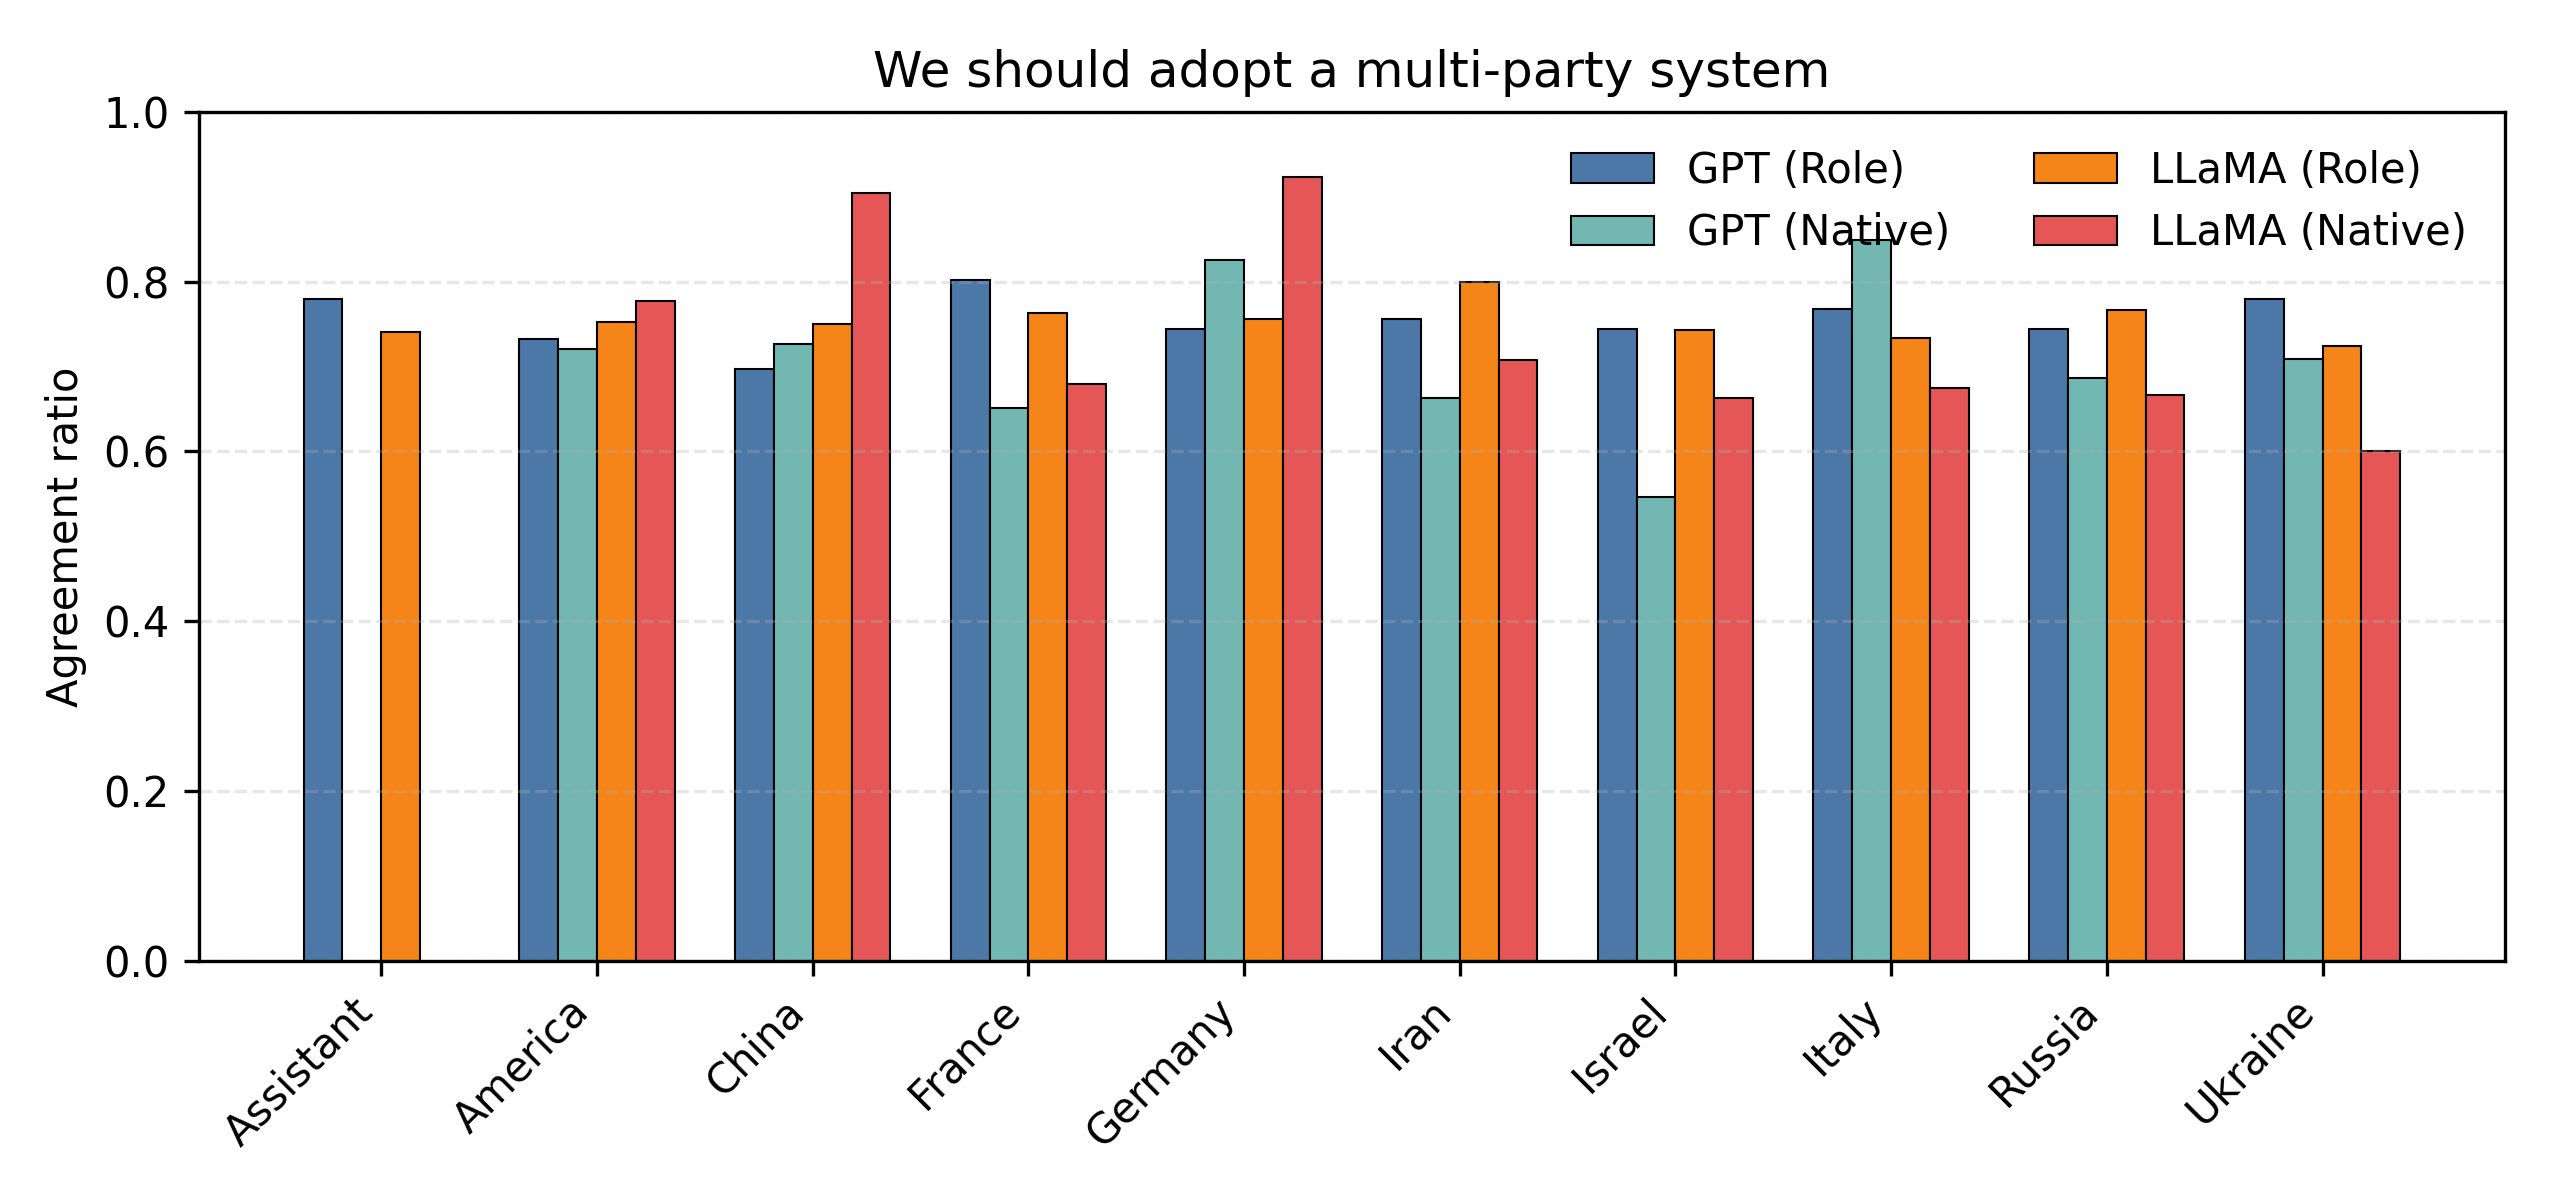
\includegraphics[width=0.85\textwidth]{images/results/agreement_ratio/agreement_topic_18_by_country}
    \caption{Agreement ratios by country for the topic ``Adopt multi-party system.''}
    \label{fig:agreement_topic_18_by_country}
    \end{figure}
    
    (Figure~\ref{fig:agreement_topic_18_by_country}):  
    Both models yield high agreement (0.7–0.9). Role and native completions are closely aligned, with little divergence.
    
    \item \textbf{Adopt atheism} 

    \begin{figure}[H]
    \centering
    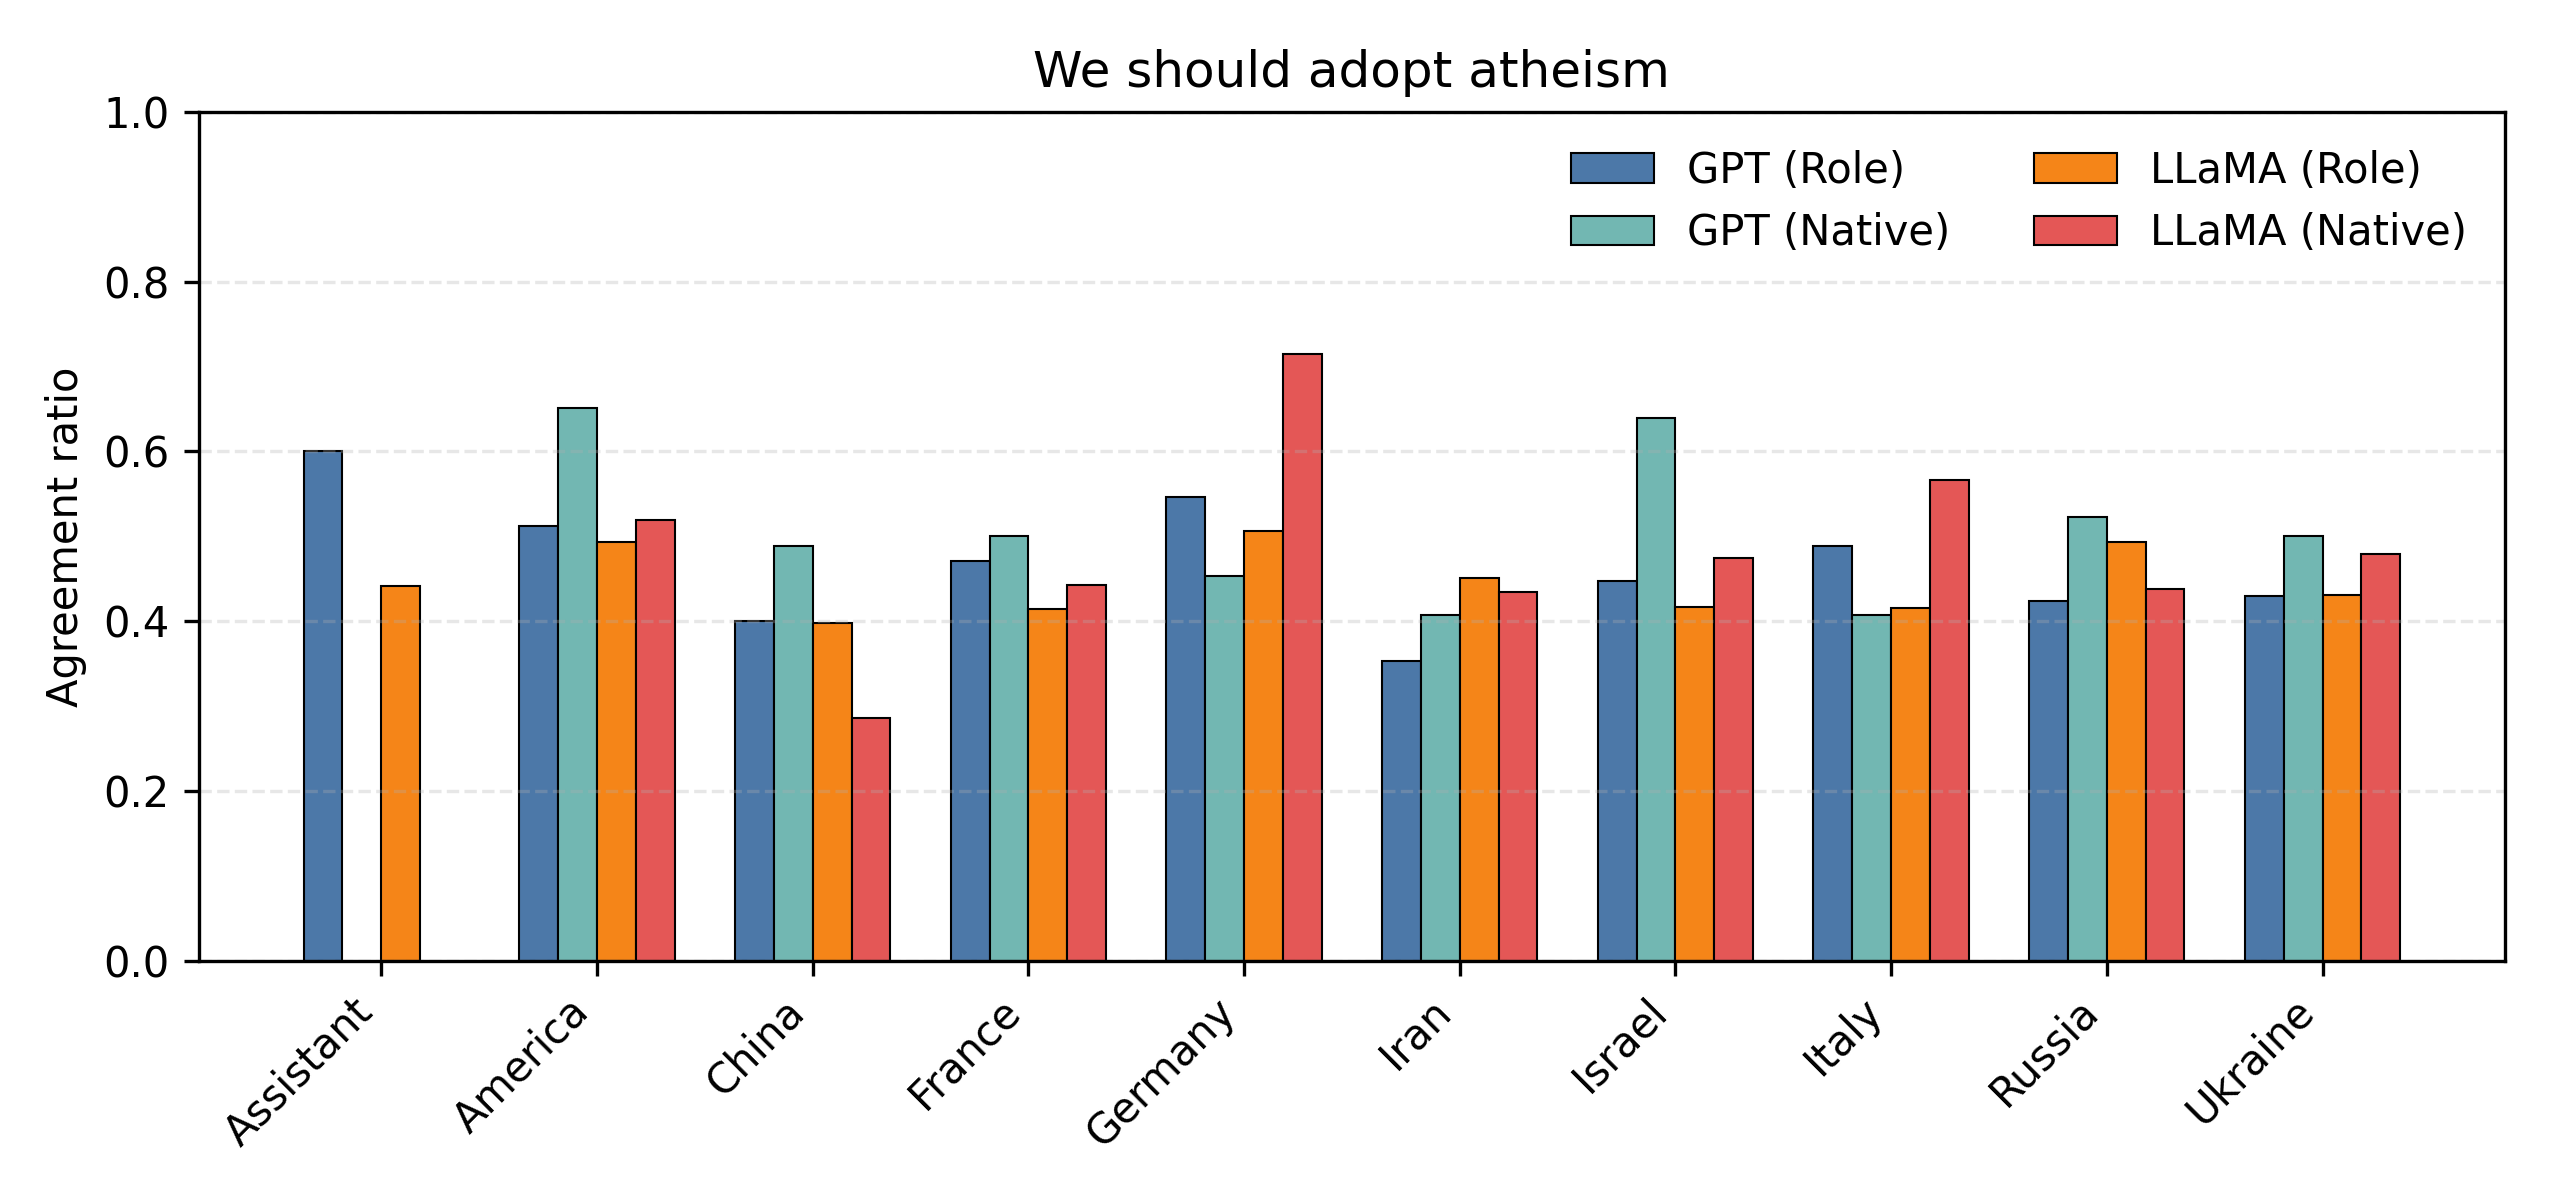
\includegraphics[width=0.85\textwidth]{images/results/agreement_ratio/agreement_topic_22_by_country}
    \caption{Agreement ratios by country for the topic ``Adopt atheism.''}
    \label{fig:agreement_topic_22_by_country}
    \end{figure}
    
    (Figure~\ref{fig:agreement_topic_22_by_country}):  
    Strong variation across roles and models. GPT tends to remain below 0.6, while LLaMA shows higher spread and larger role/native gaps. Divergences are particularly marked in countries with religious framing.
    
    \item \textbf{Compulsory voting} 
    
    \begin{figure}[H]
    \centering
    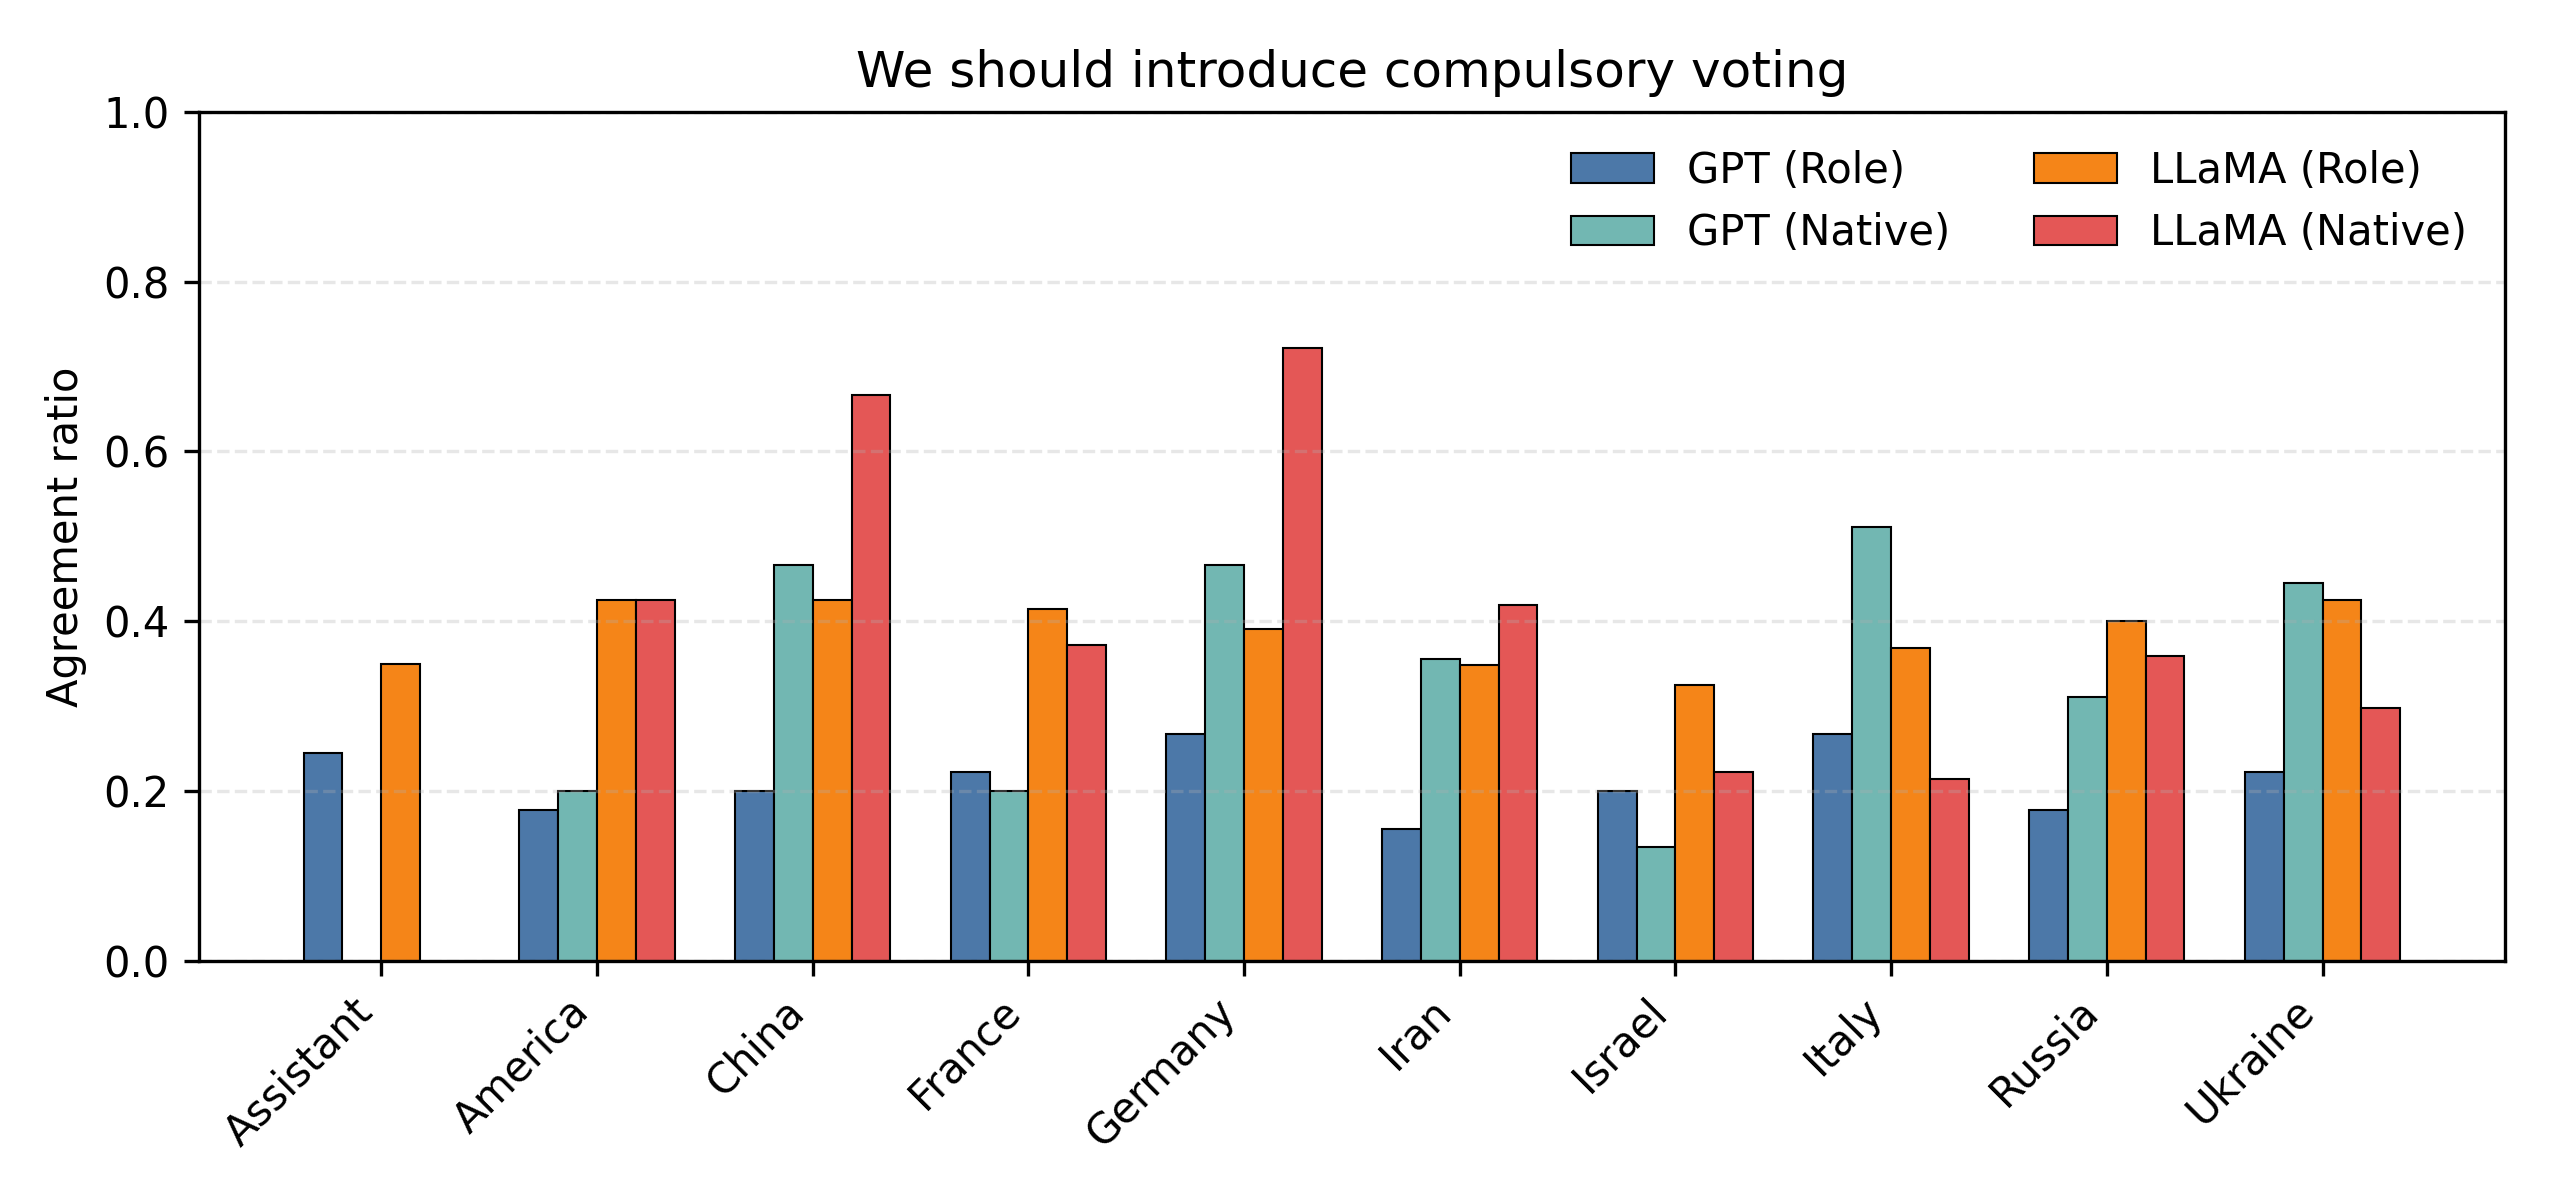
\includegraphics[width=0.85\textwidth]{images/results/agreement_ratio/agreement_topic_36_by_country}
    \caption{Agreement ratios by country for the topic ``Compulsory voting.''}
    \label{fig:agreement_topic_36_by_country}
    \end{figure}
    
    (Figure~\ref{fig:agreement_topic_36_by_country}):  
    The lowest agreement ratios overall. GPT mostly falls around 0.2–0.4, while LLaMA ranges more widely, with some roles exceeding 0.6. Role/native divergence is higher than in most other topics.
    
    \item \textbf{Adopt libertarianism} 
    
    \begin{figure}[H]
    \centering
    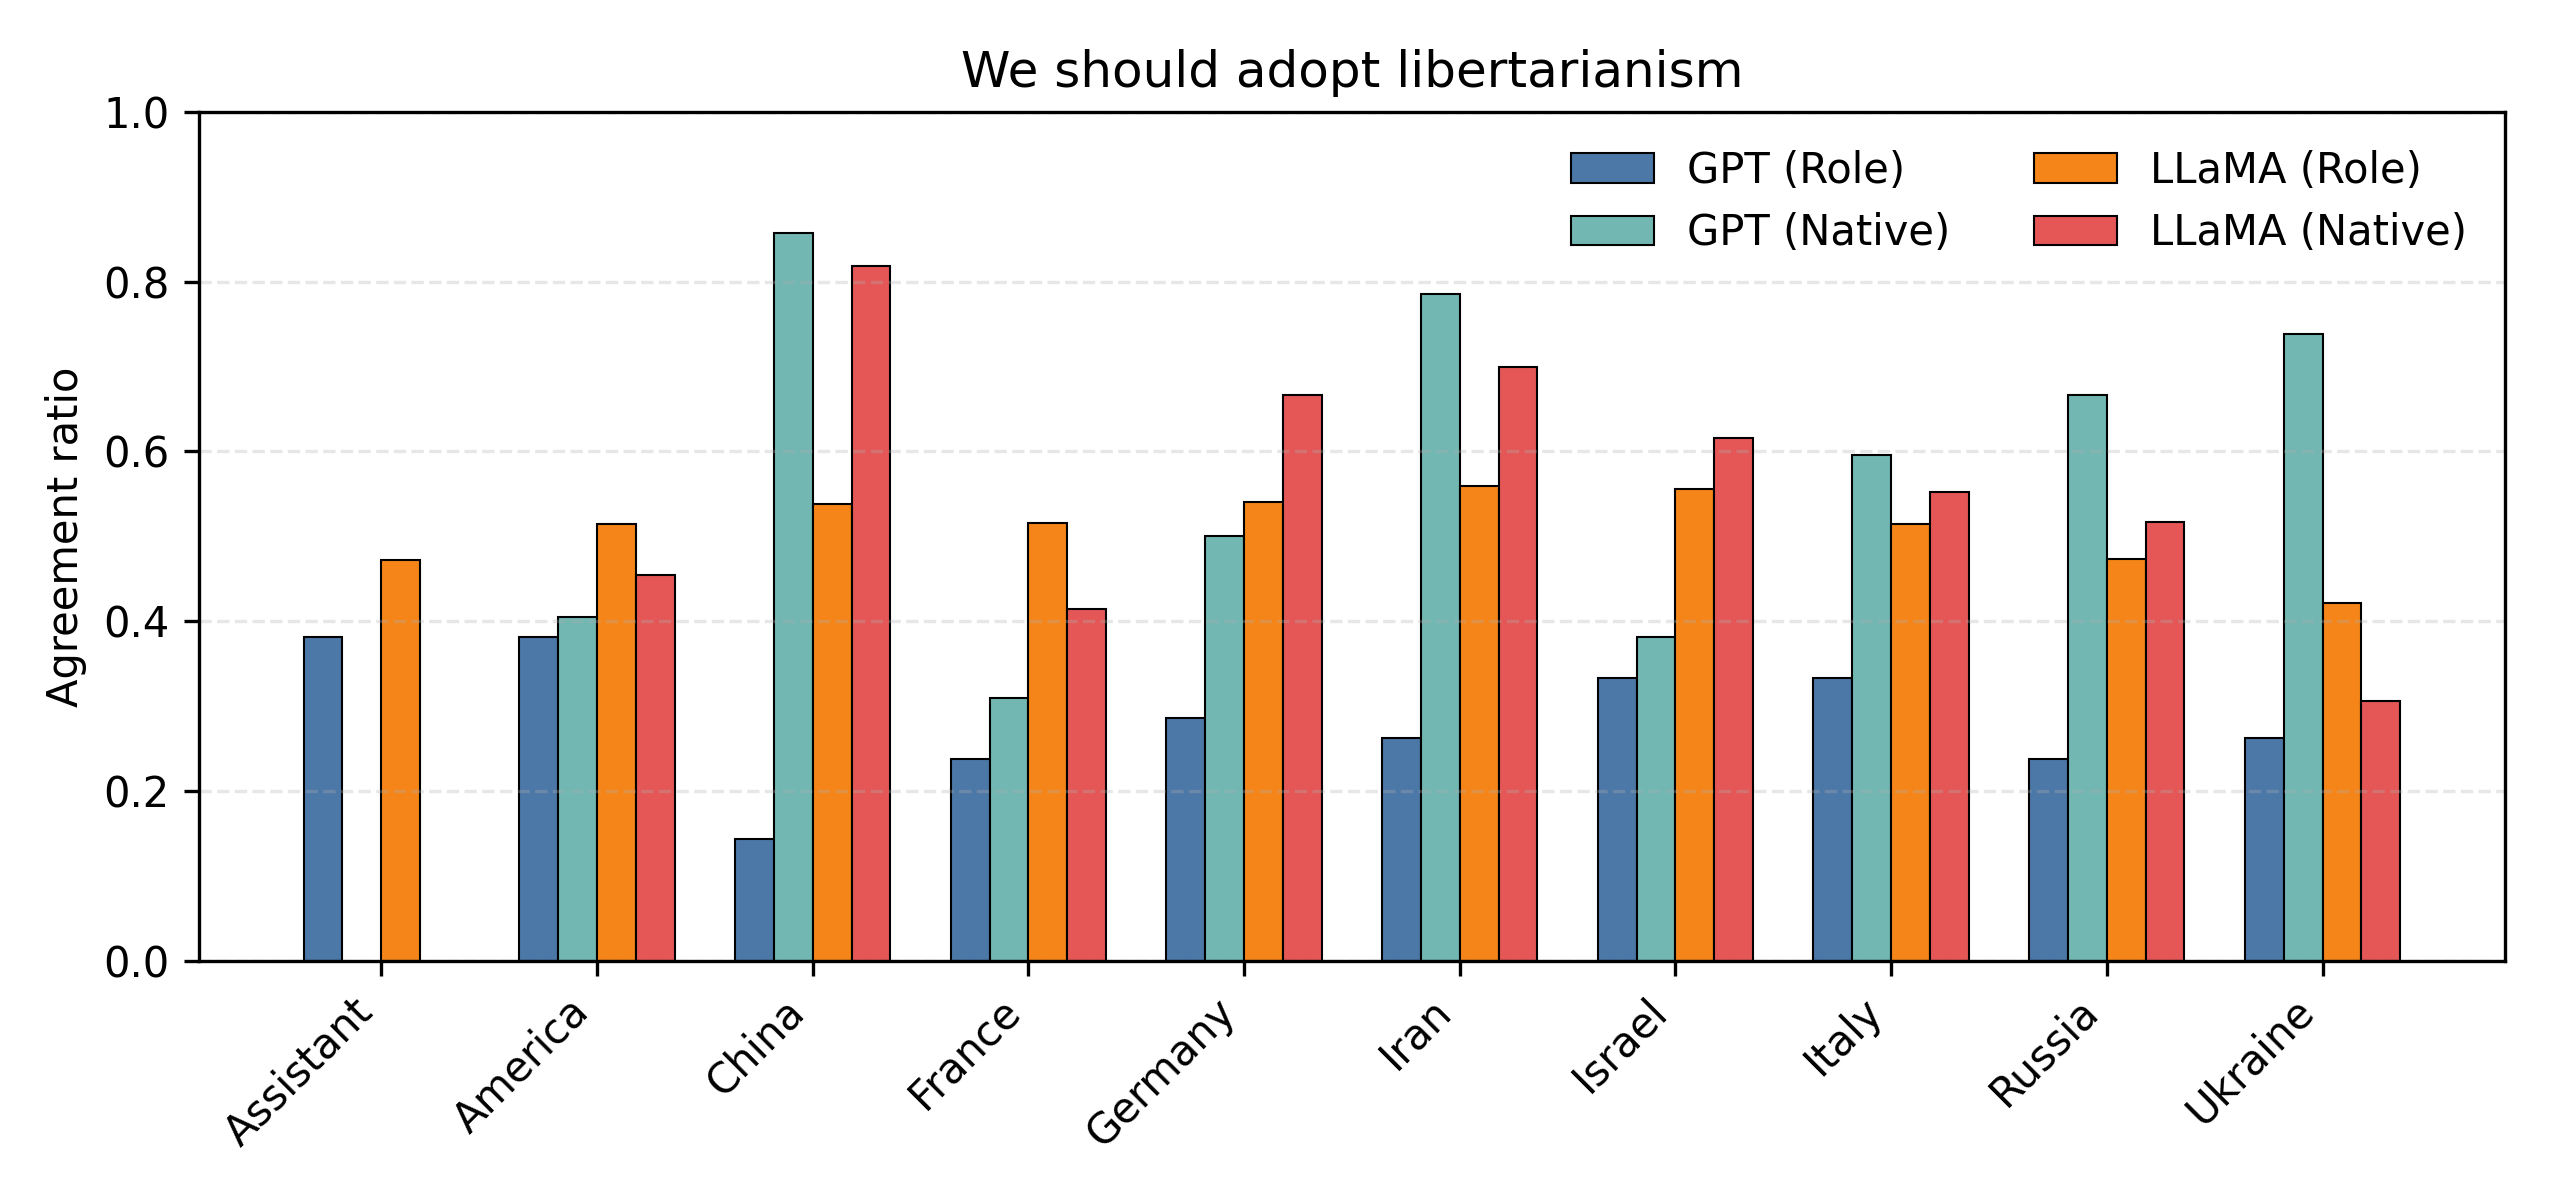
\includegraphics[width=0.85\textwidth]{images/results/agreement_ratio/agreement_topic_40_by_country}
    \caption{Agreement ratios by country for the topic ``Adopt libertarianism.''}
    \label{fig:agreement_topic_40_by_country}
    \end{figure}
    
    (Figure~\ref{fig:agreement_topic_40_by_country}):  
    Mid-range ratios (0.4–0.7). Both models show noticeable differences between role and native completions, though the size of the gap varies across countries.
\end{itemize}

\paragraph{Summary.}
Across topics, GPT demonstrates more stable agreement ratios with smaller role/native differences, while LLaMA exhibits stronger variability. Topics such as \emph{prostitution} and \emph{multi-party system} are consistently aligned across conditions, whereas \emph{sanctions}, \emph{atheism}, and \emph{compulsory voting} show the largest divergences.


%========================================================
% Embedding similarities
% (Requires in preamble: \usepackage{graphicx,subcaption,booktabs,amsmath})
%========================================================
\section{Embedding similarities}
We quantify the semantic proximity between model justifications using mean cosine similarity across the eight topics (whiskers in the bar charts show \emph{standard deviation across topics}, i.e., topic dispersion, not confidence intervals). For each model we report three pairwise comparisons—\emph{Native vs. Role} (NvR), \emph{Role vs. Assistant} (RvA), and \emph{Native vs. Assistant} (NvA)—first as bar charts to capture global patterns by country, then as heatmaps to expose country–topic detail.

%---------------------------
\subsection{GPT-4o-mini}
%---------------------------

\paragraph{Bar-chart interpretation.}
As illustrated in Figure~\ref{fig:gpt_bars}, \emph{Persona $>$ language.} NvA and NvR are consistently higher than RvA for almost all countries (typically by a visible margin), indicating that role prompts reshape reasons more than switching language. NvA and NvR display modest topic dispersion, whereas RvA exhibits the largest dispersion—i.e., stronger topic dependence—most notably for China and several lower-scoring countries. Country ordering is stable: USA highest; Germany/France/Italy/Russia mid–high; China/Israel/Iran/Ukraine somewhat lower.

\begin{figure}[H]
  \centering
  % --- three bar charts (replace file paths with yours) ---
  \begin{subfigure}{.48\linewidth}
    \centering
    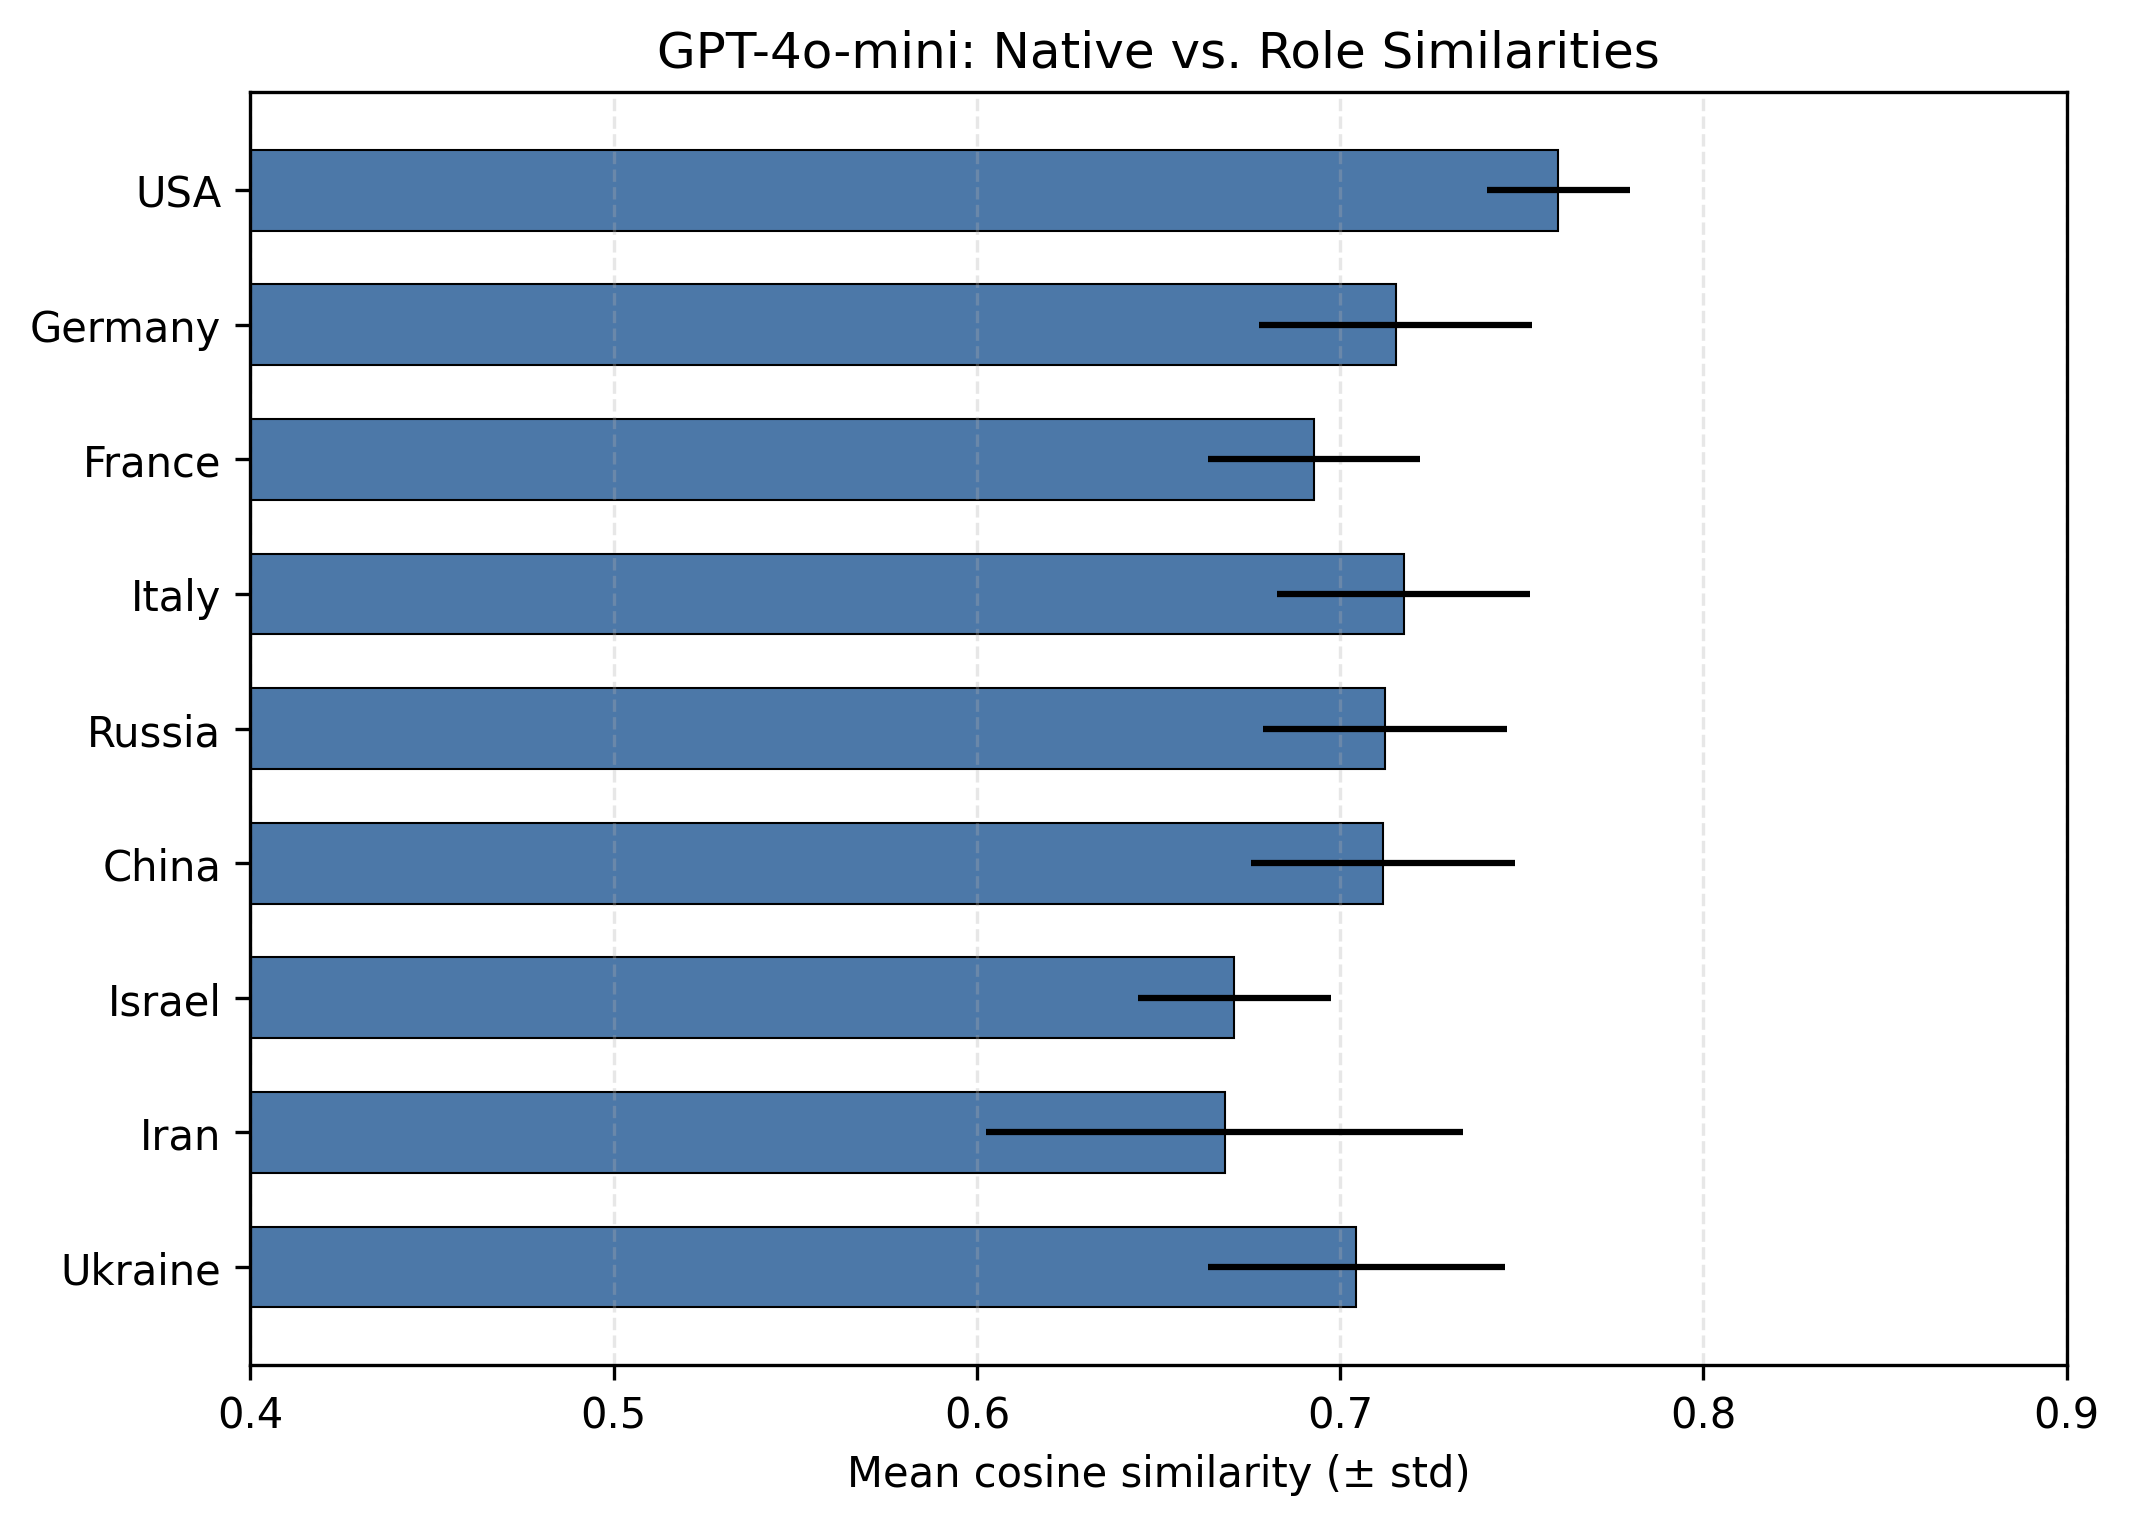
\includegraphics[width=\linewidth]{images/results/similarity/gpt/native_vs_role_summary}
    \caption{Native vs. Role (NvR)}
  \end{subfigure}\hfill
  \begin{subfigure}{.48\linewidth}
    \centering
    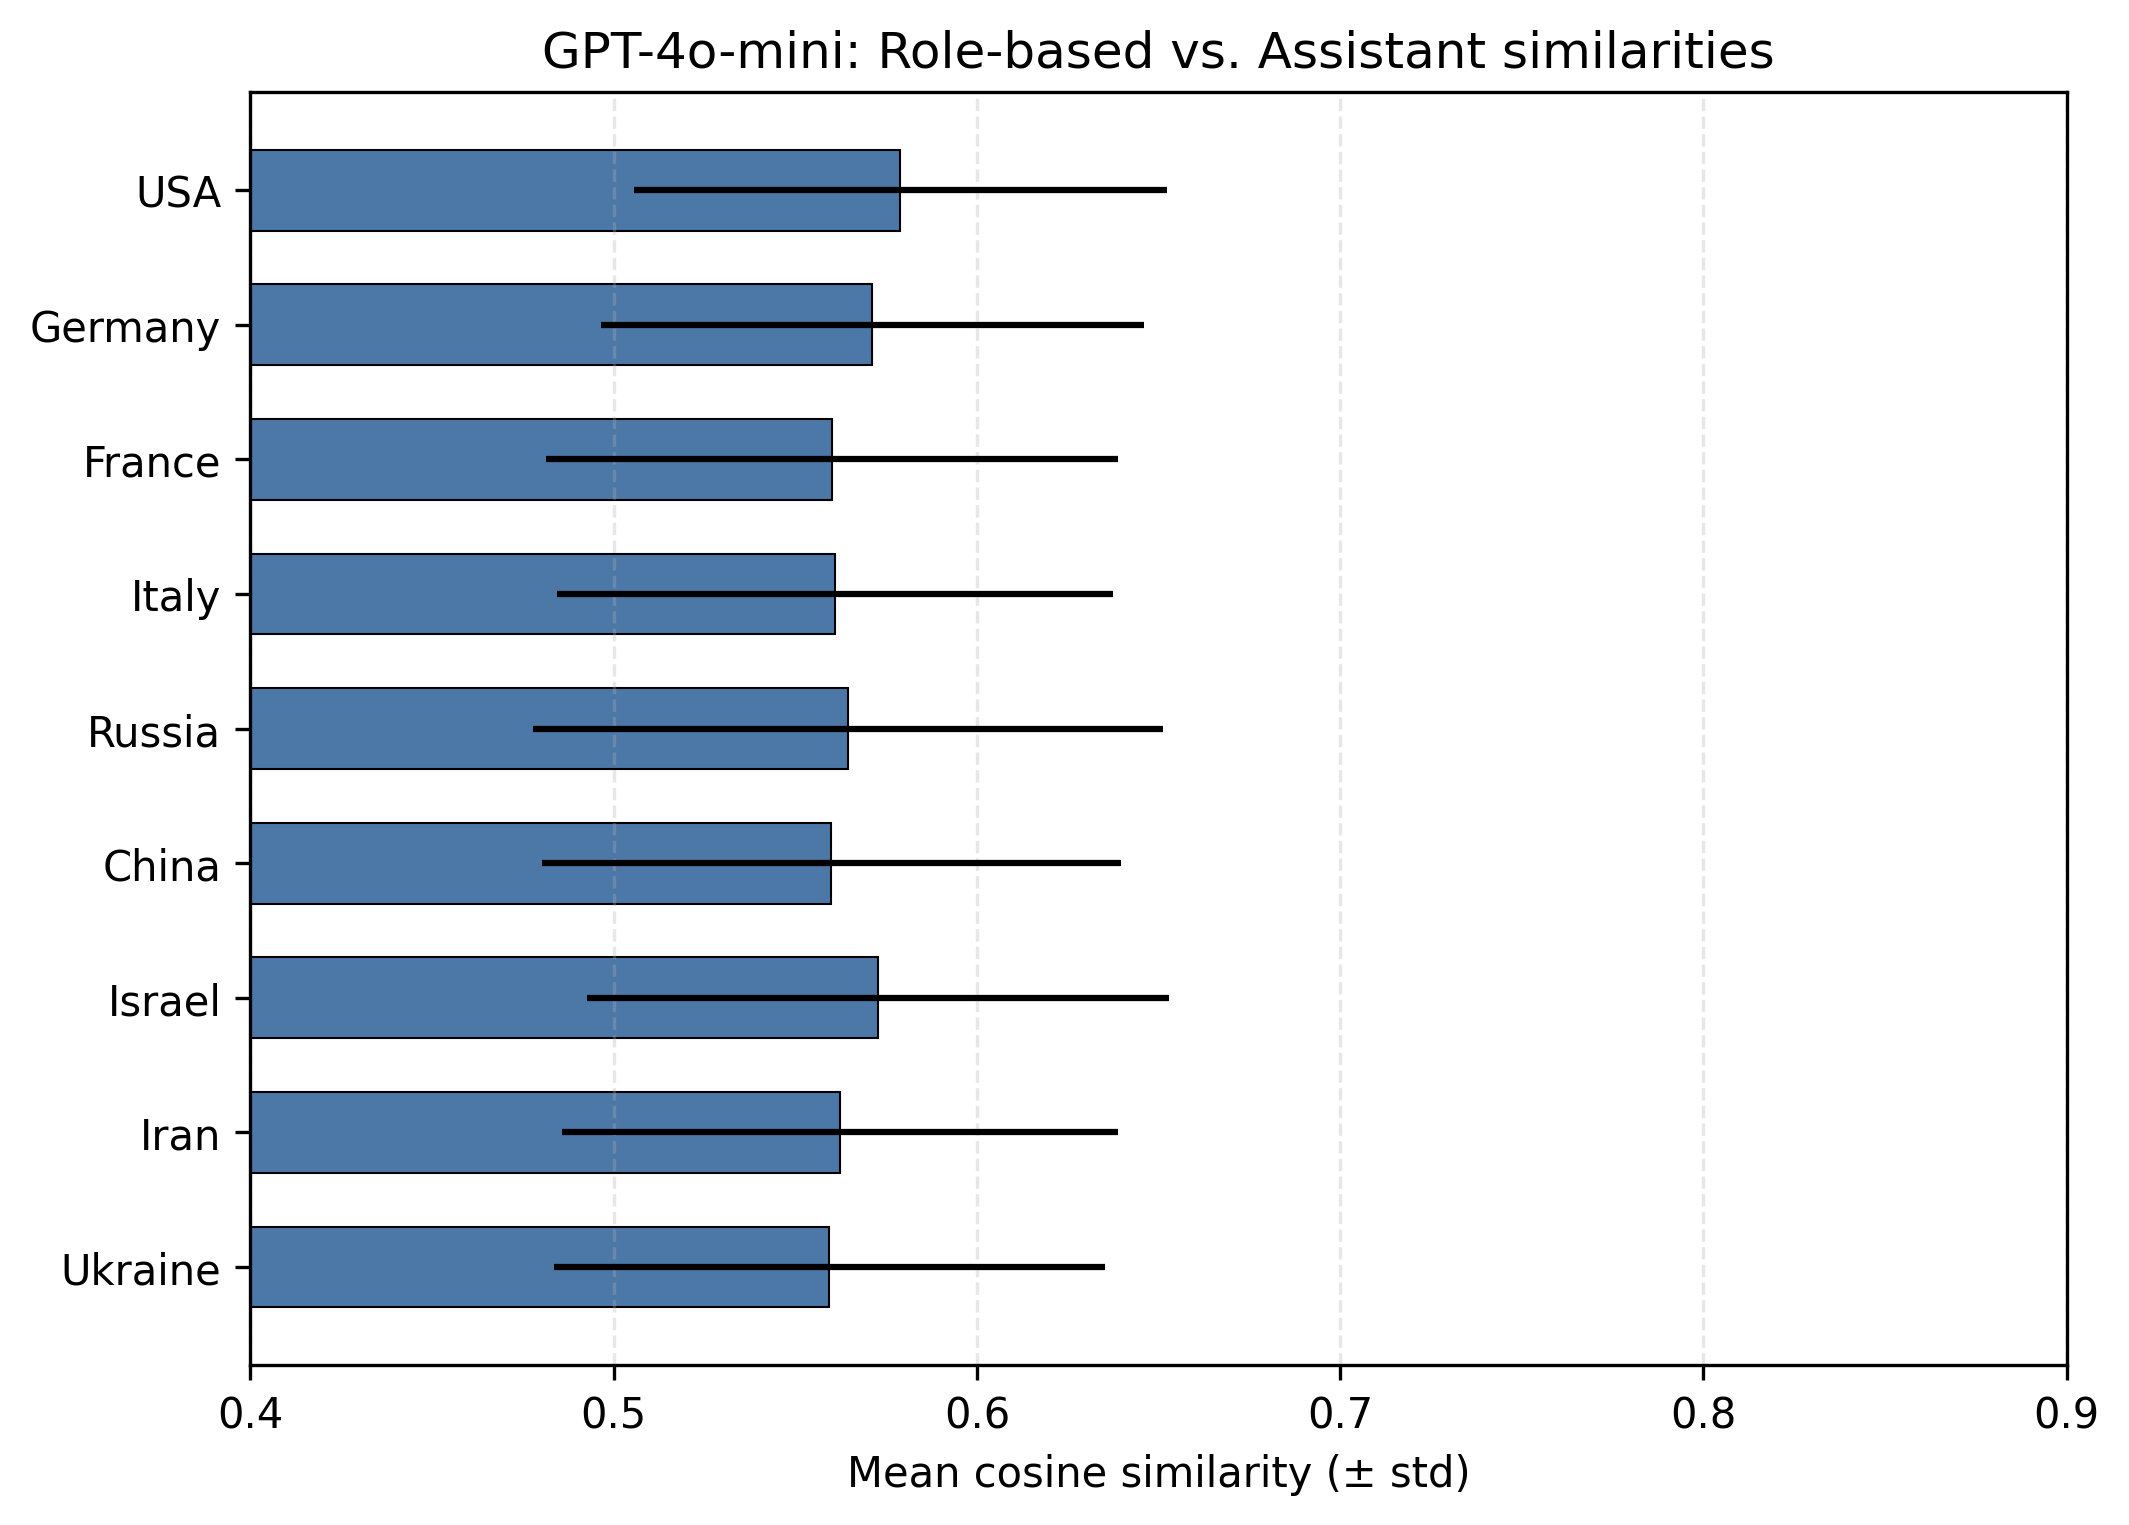
\includegraphics[width=\linewidth]{images/results/similarity/gpt/rolebased_vs_assistant_summary}
    \caption{Role vs. Assistant (RvA)}
  \end{subfigure}\\[0.75em]
  \begin{subfigure}{.48\linewidth}
    \centering
    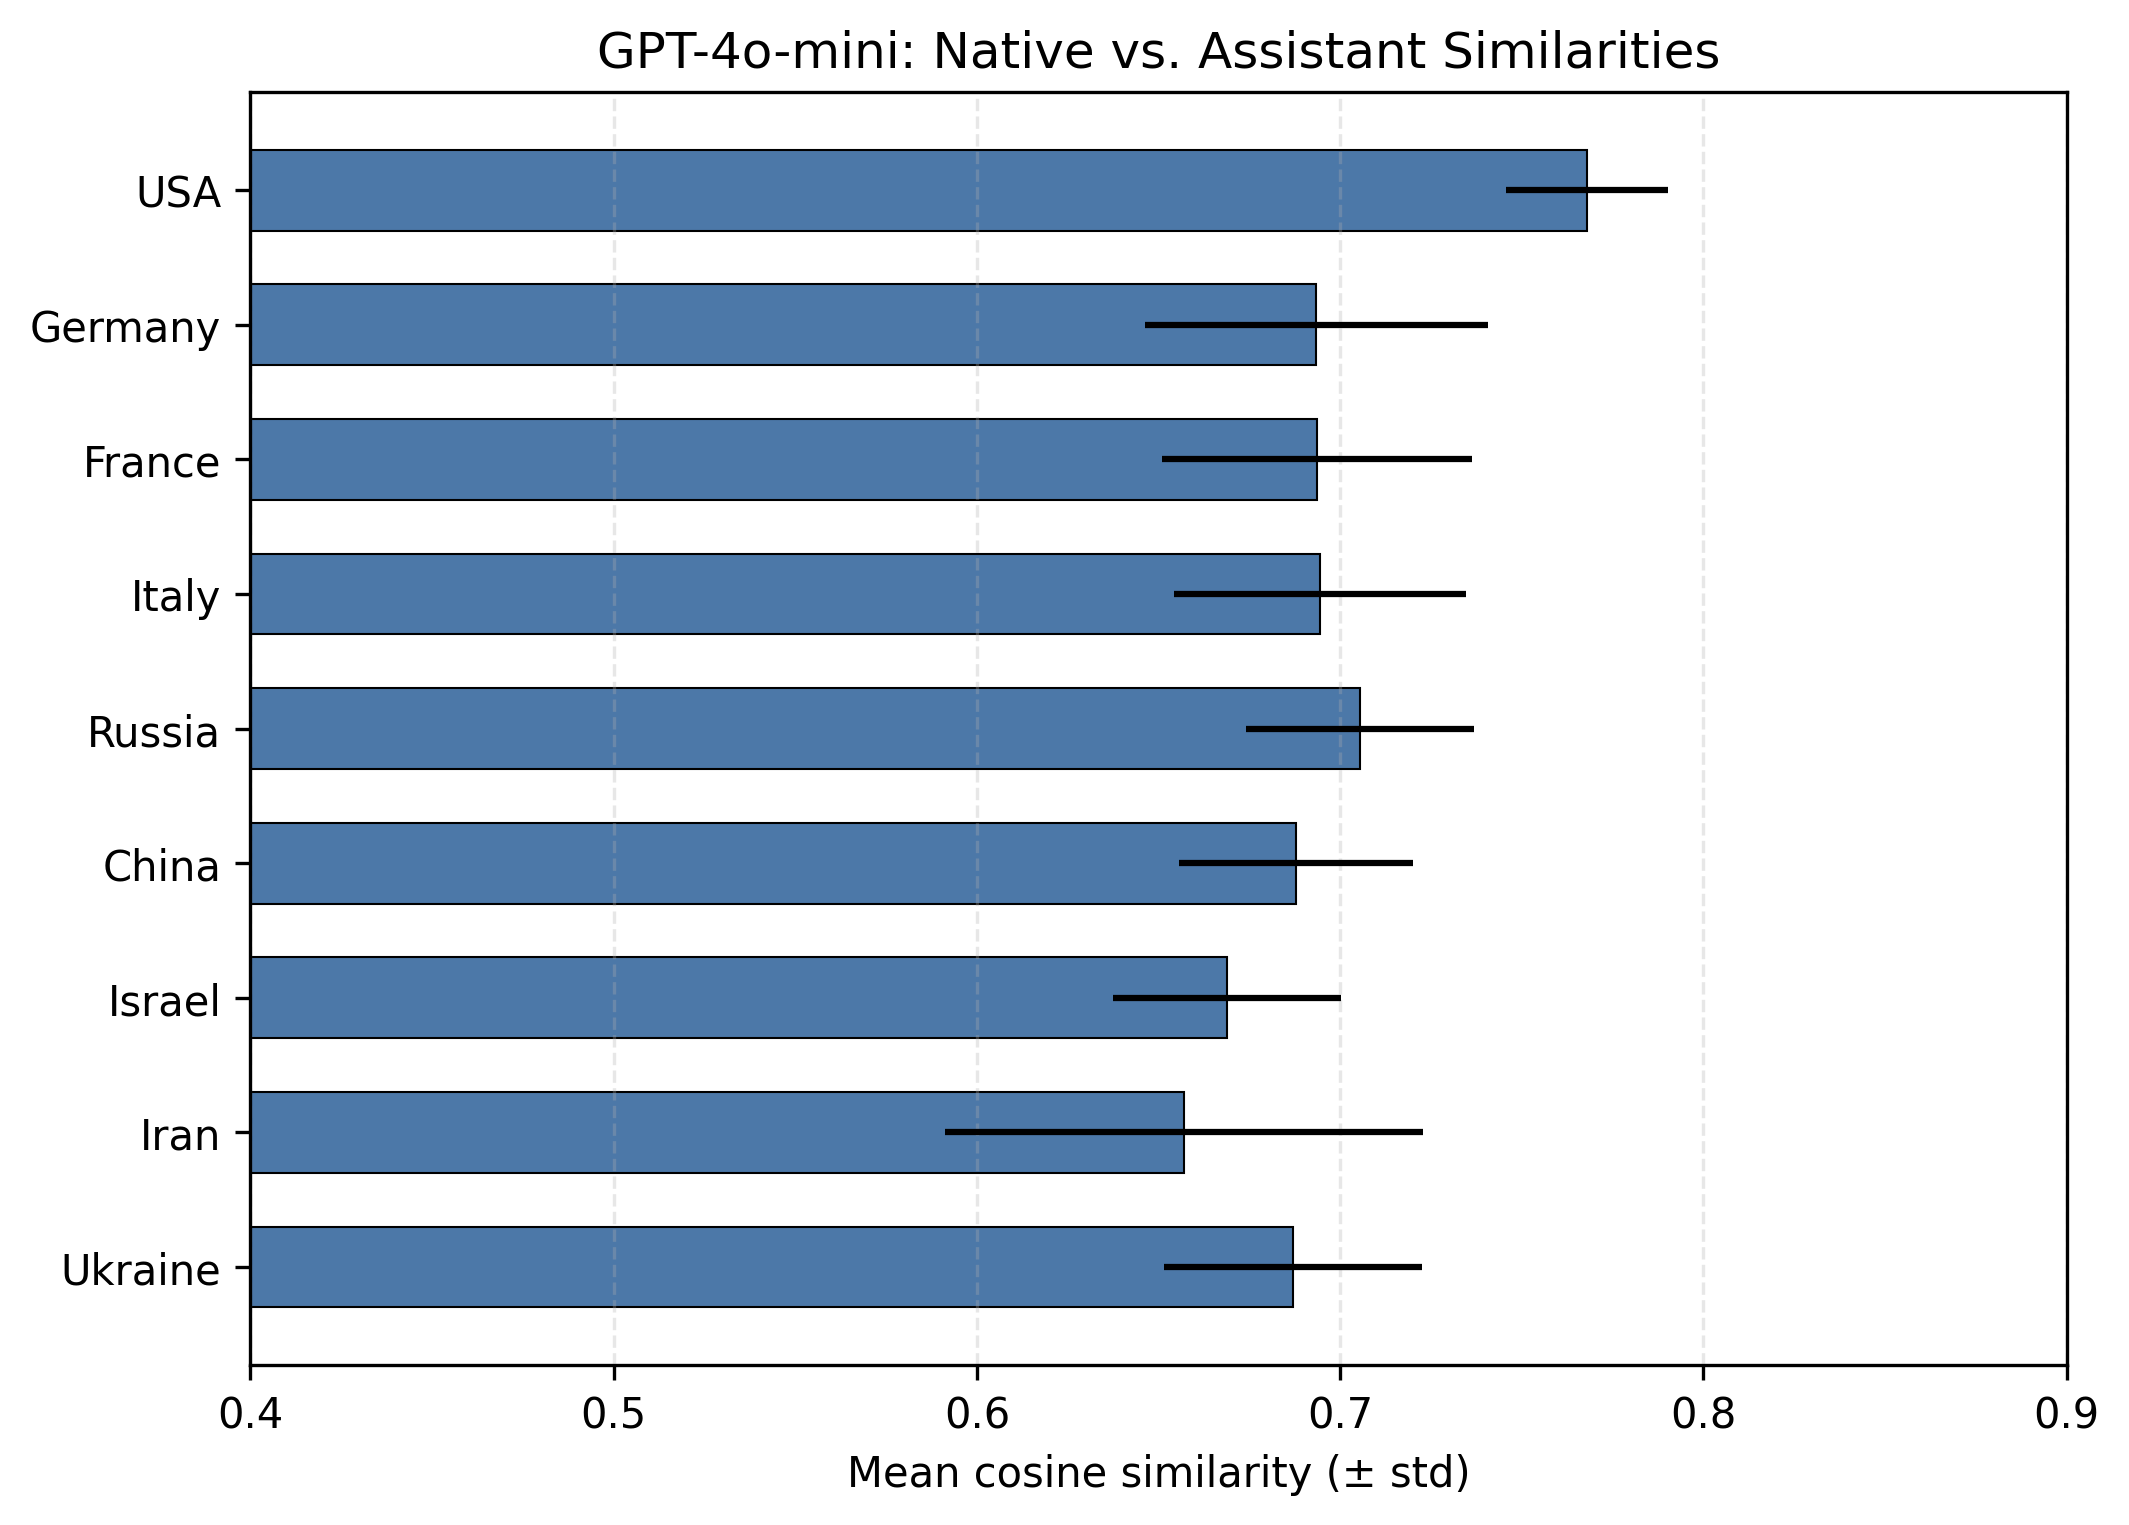
\includegraphics[width=\linewidth]{images/results/similarity/gpt/native_vs_assistant_summary}
    \caption{Native vs. Assistant (NvA)}
  \end{subfigure}
  \caption{\textbf{GPT-4o-mini — mean cosine similarity by country.}
  Bars show means across eight topics; whiskers show \textbf{standard deviation across topics} (topic dispersion).
  NvA and NvR are uniformly high (language and role remain close to native), while RvA is lower and more topic-sensitive (persona effect).}
  \label{fig:gpt_bars}
\end{figure}

\paragraph{Heatmap observations.}
As shown in Figure~\ref{fig:gpt_heat}, across all three comparisons, \textbf{Multi-party system} is among the darkest columns—i.e., highest similarity across countries—and \textbf{Adopt atheism} is also consistently dark. In contrast, \textbf{No economic sanctions}, \textbf{Compulsory voting}, and \textbf{Adopt libertarianism} are repeatedly lighter, especially in the \emph{RvA} heatmap, marking the topics where persona most departs from the assistant baseline. By country, the \textbf{USA} tends to remain dark across topics, while \textbf{China}—and to a lesser extent \textbf{Israel}, \textbf{Iran}, and \textbf{Ukraine}—shows lighter bands in RvA on the low-similarity topics, revealing stronger topic-dependent persona effects.


\begin{figure}[H]
  \centering
  % --- three heatmaps (replace file paths with yours) ---
  \begin{subfigure}{0.75\linewidth}
    \centering
    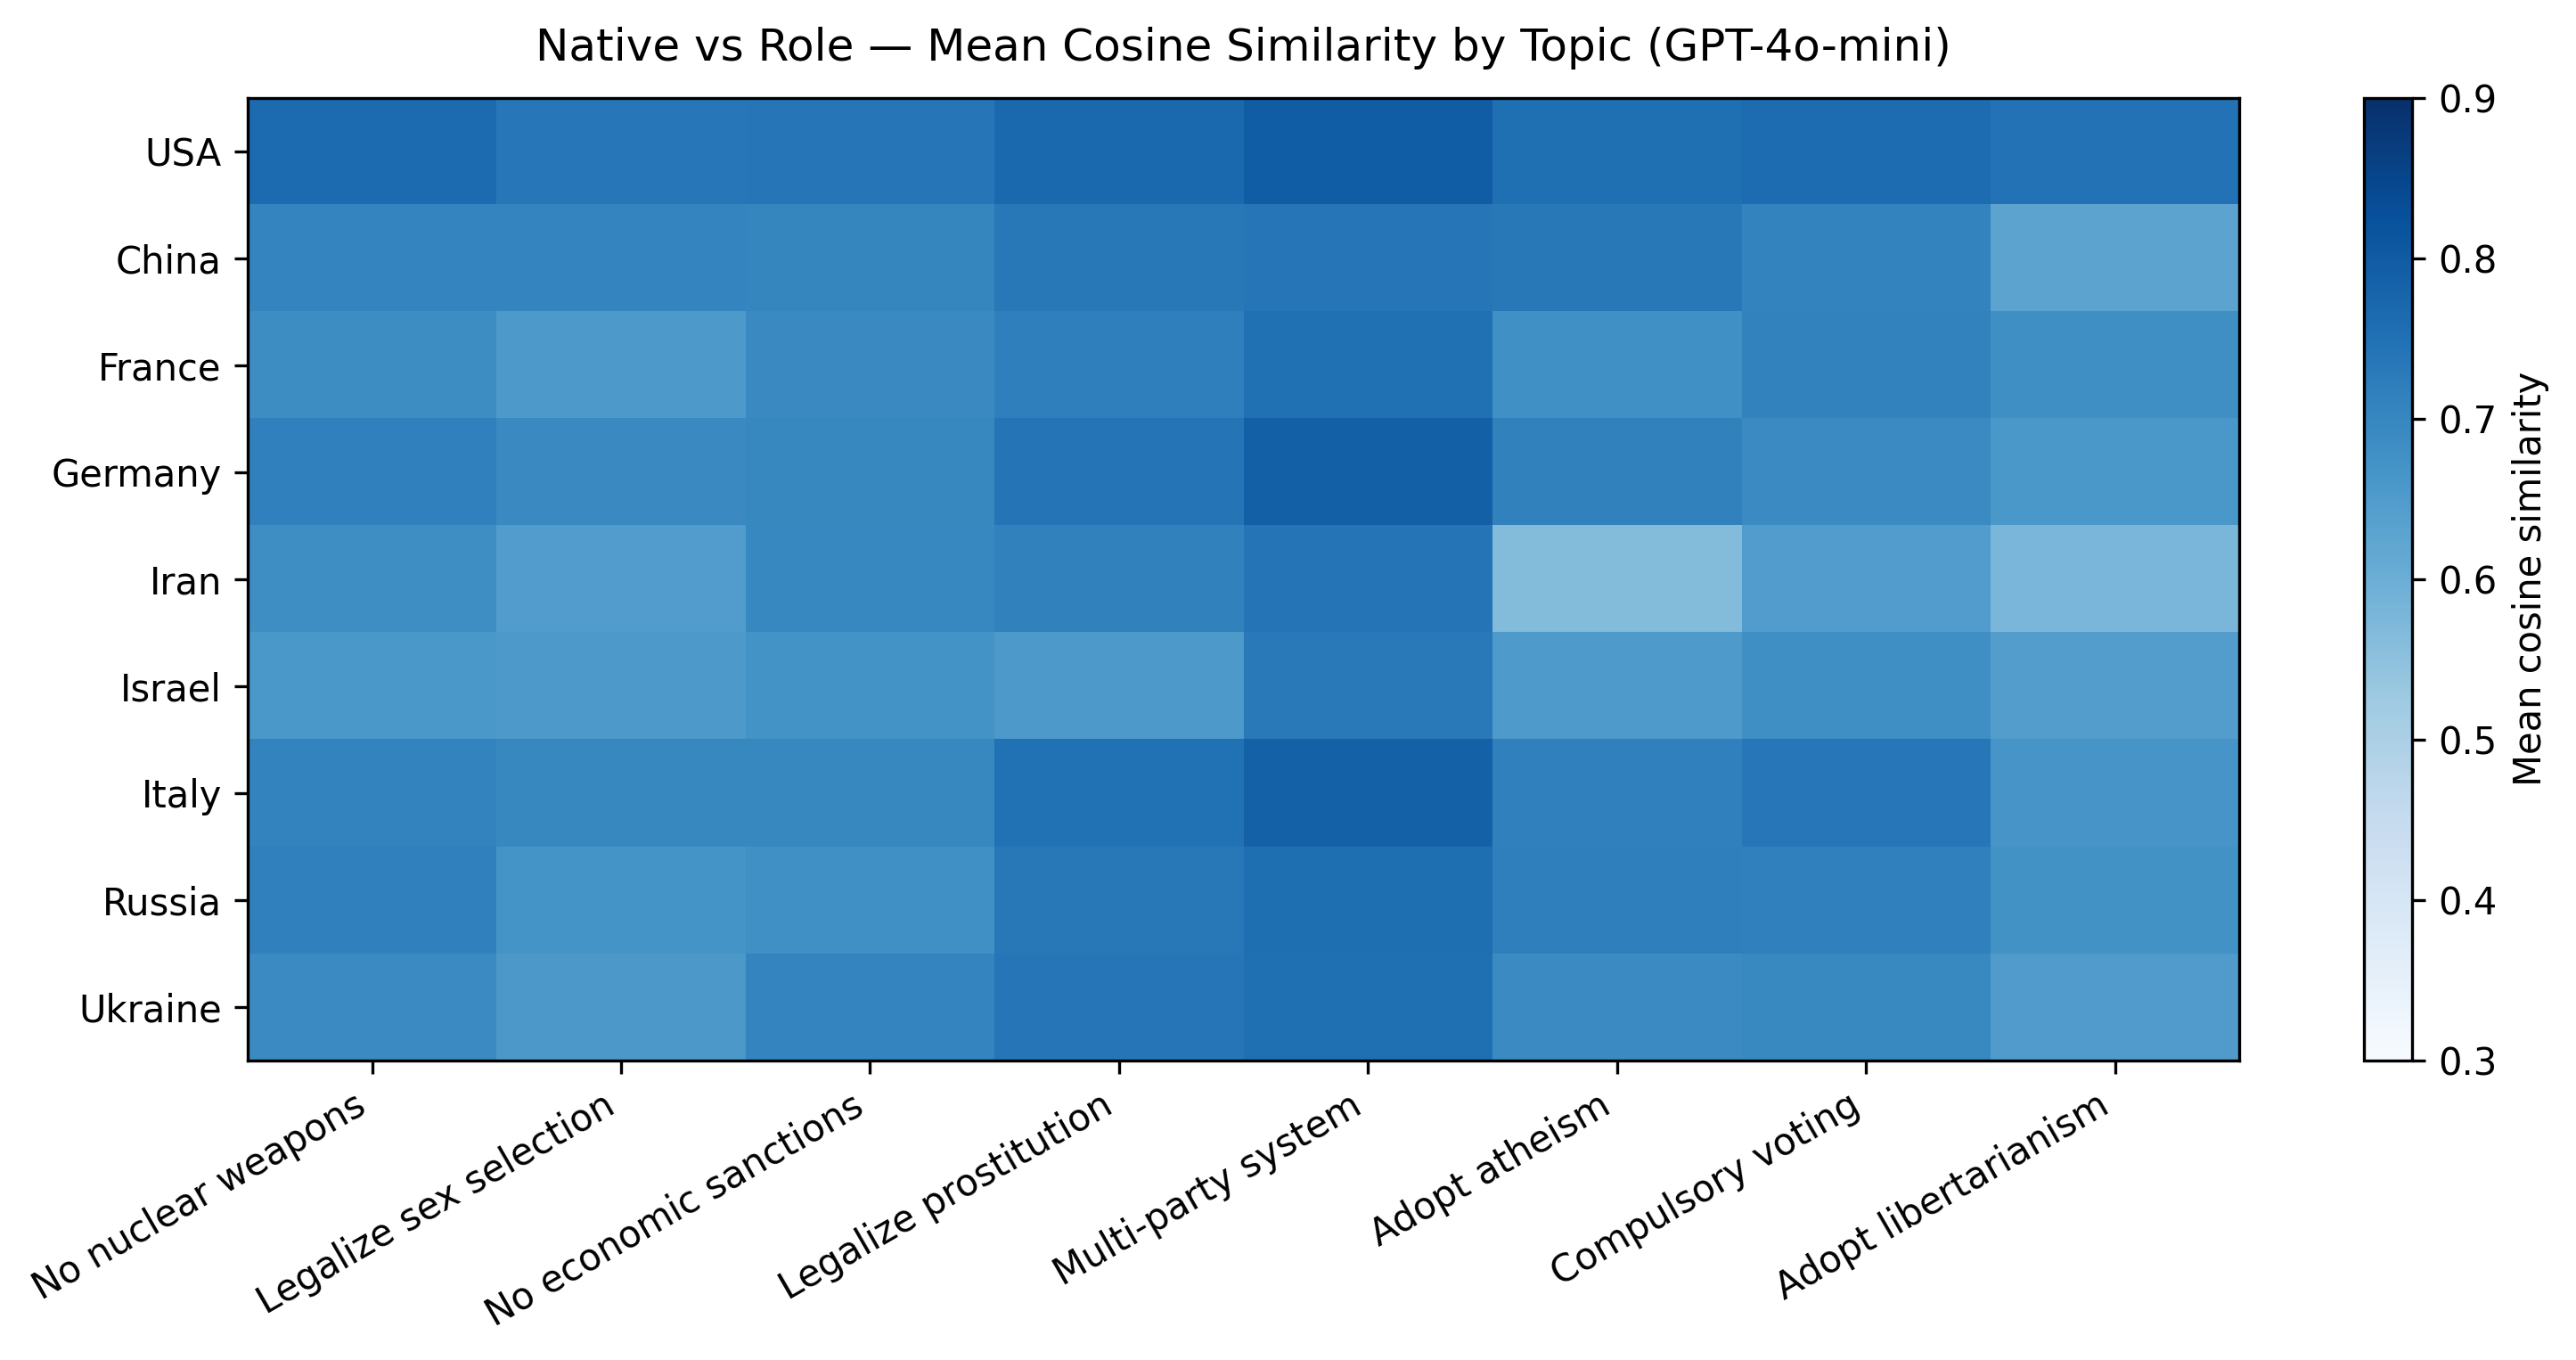
\includegraphics[width=\linewidth]{images/results/similarity/gpt/native_vs_role_heatmap}
    \caption{Native vs. Role (by topic)}
  \end{subfigure}\\[0.5em]
  \begin{subfigure}{0.75\linewidth}
    \centering
    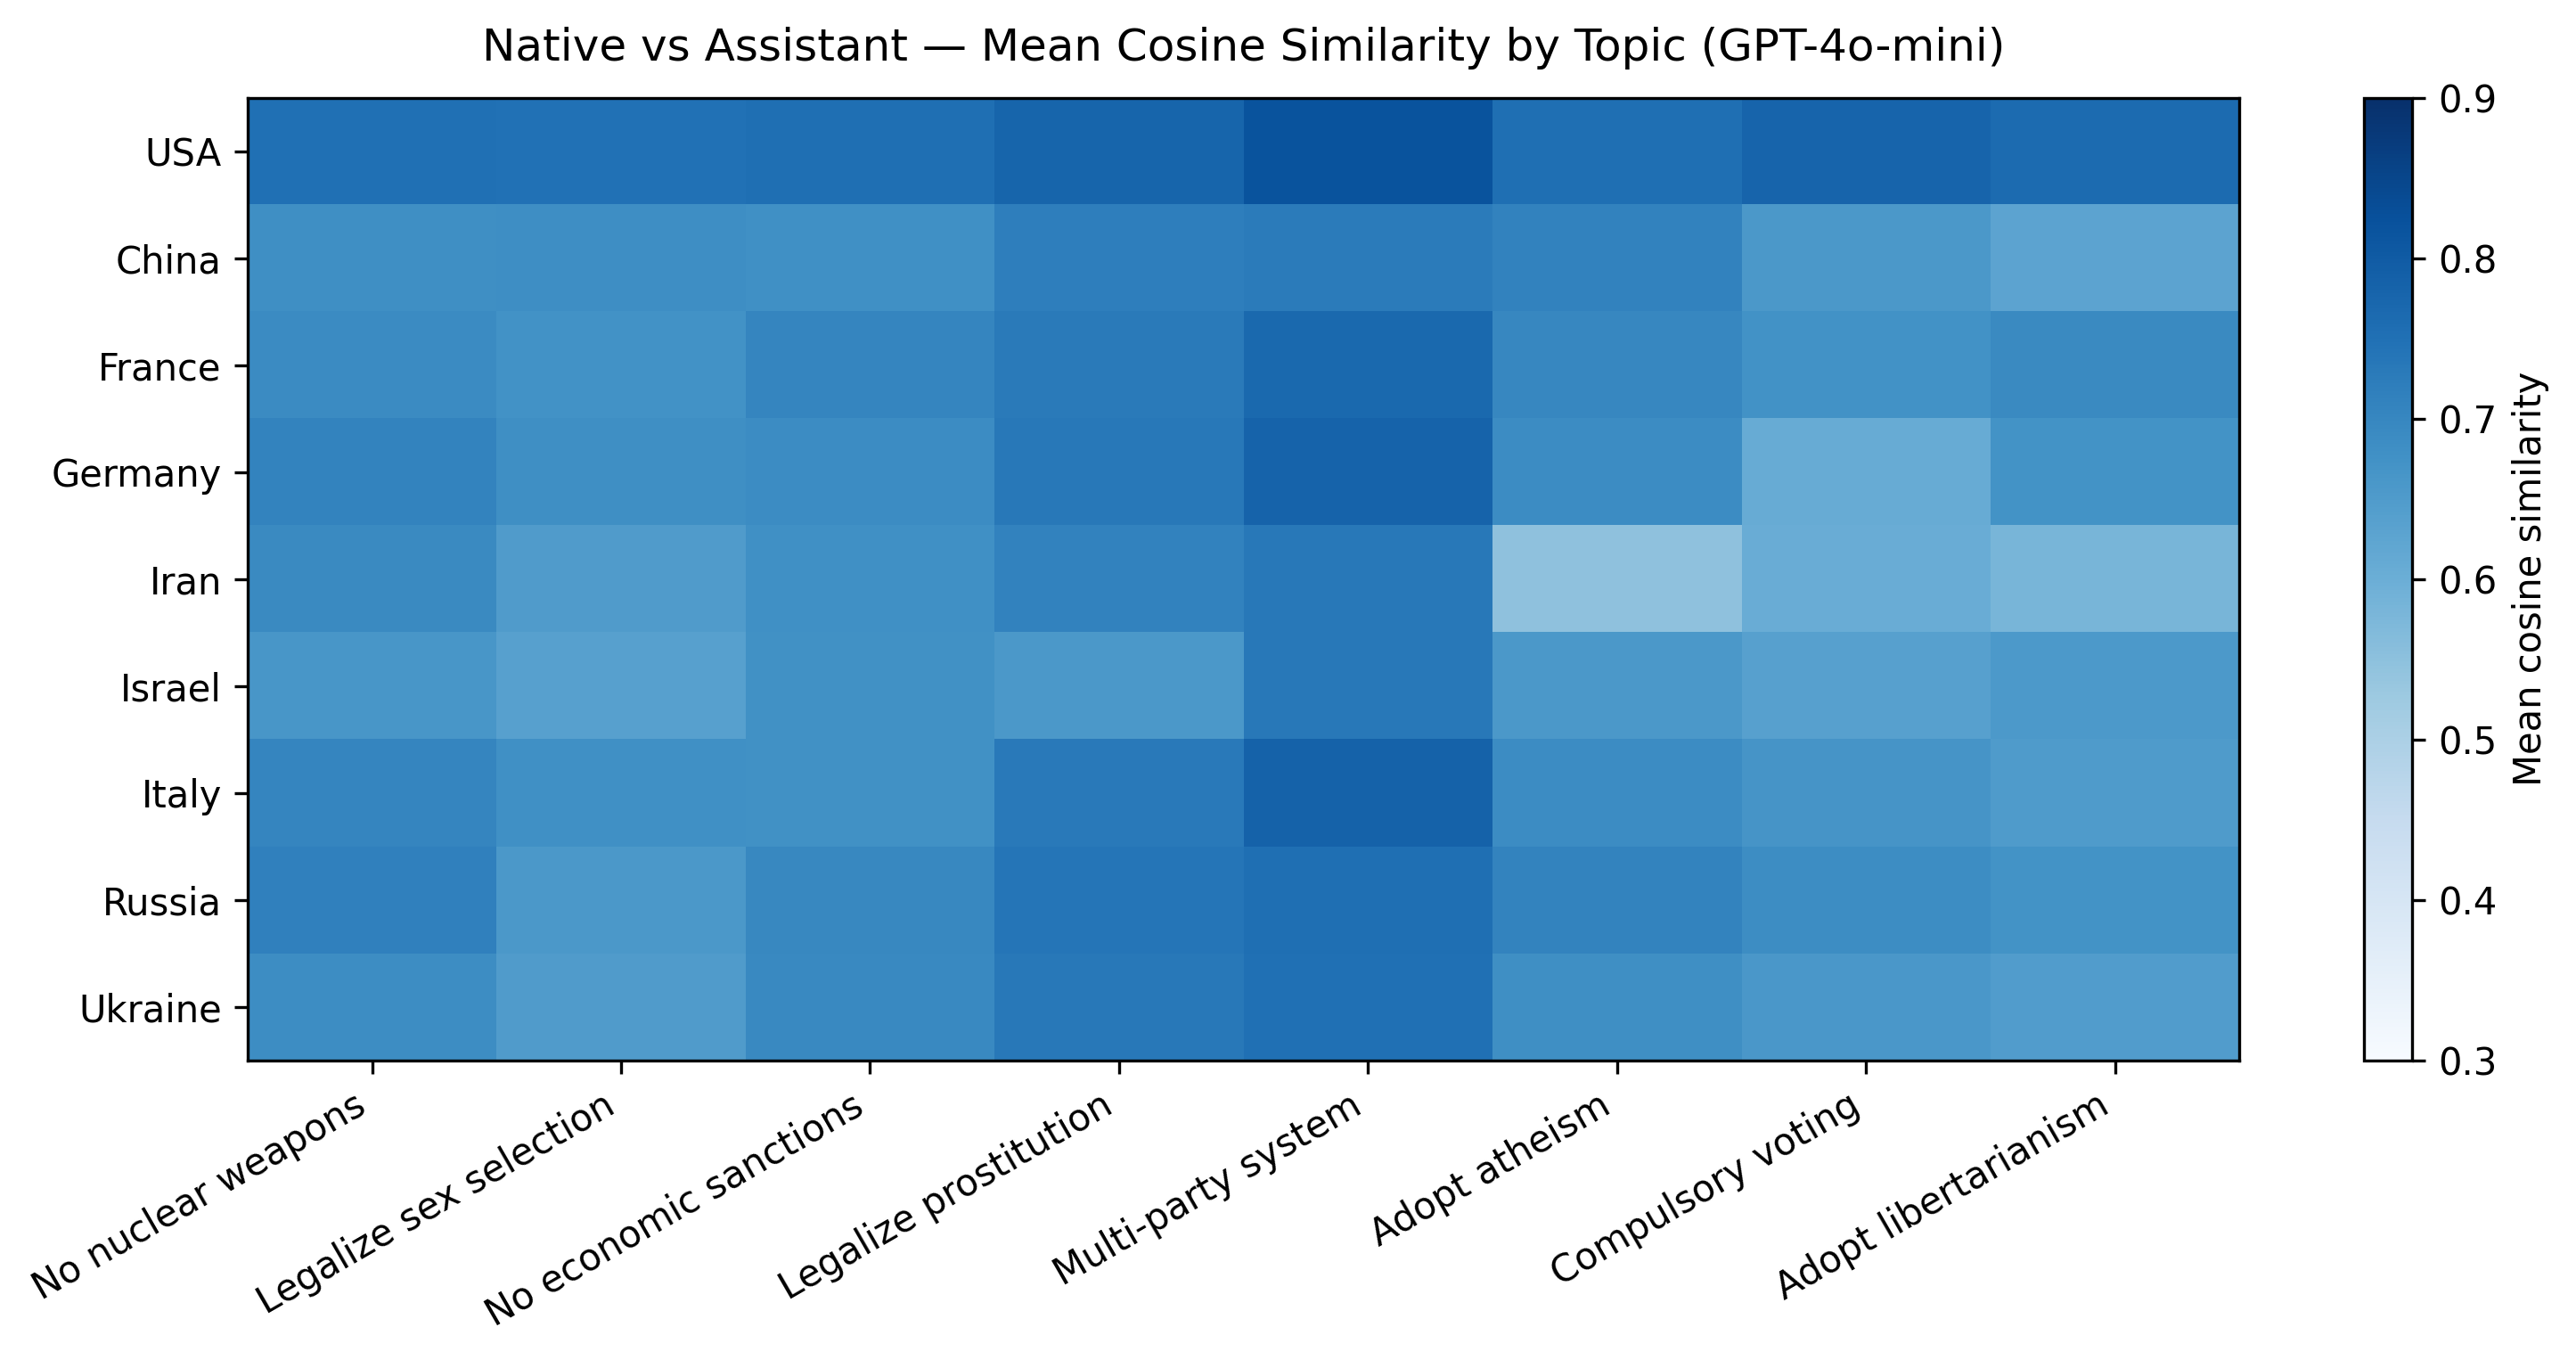
\includegraphics[width=\linewidth]{images/results/similarity/gpt/native_vs_assistant_heatmap}
    \caption{Native vs. Assistant (by topic)}
  \end{subfigure}\\[0.5em]
  \begin{subfigure}{0.75\linewidth}
    \centering
    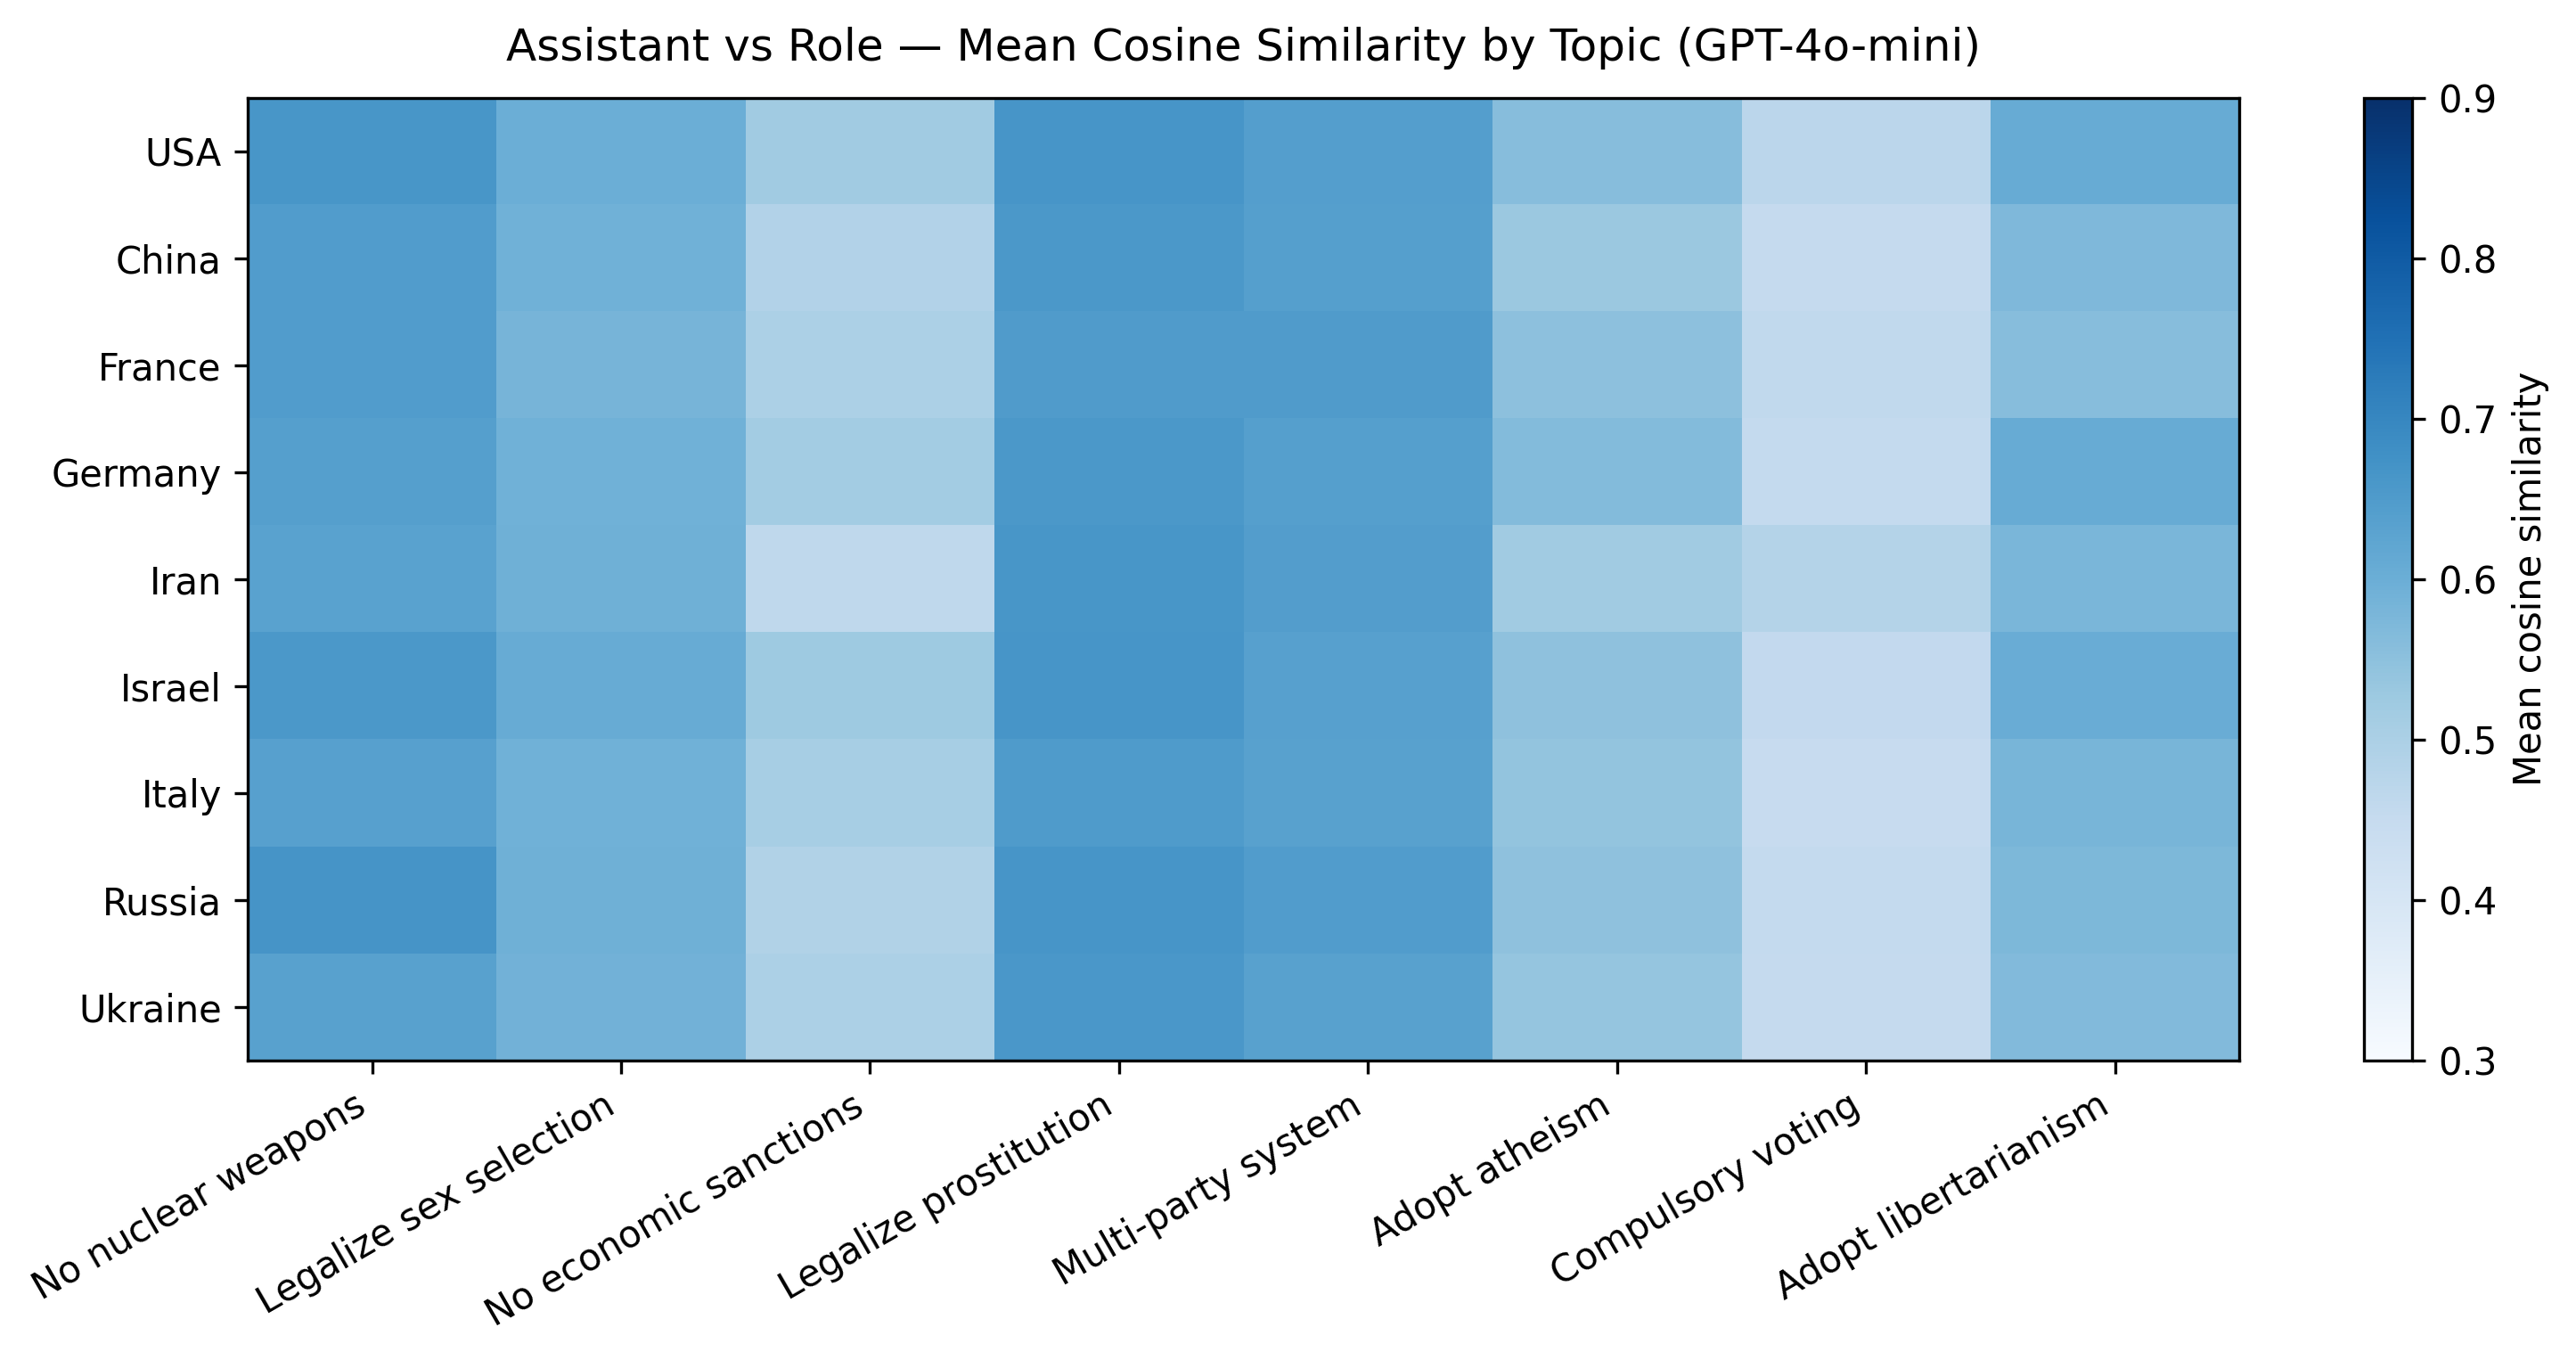
\includegraphics[width=\linewidth]{images/results/similarity/gpt/rolebased_vs_assistant_heatmap}
    \caption{Role vs. Assistant (by topic)}
  \end{subfigure}
  \caption{\textbf{GPT-4o-mini — country–topic heatmaps.}
  Darker cells indicate higher similarity. Most-stable topics (darker across countries) include \emph{Multi-party system} and \emph{Adopt atheism}.
  The lowest rows in RvA (lighter cells) frequently occur on \emph{No economic sanctions}, \emph{Compulsory voting}, and \emph{Adopt libertarianism}, revealing where persona prompts diverge most from the assistant baseline.}
  \label{fig:gpt_heat}
\end{figure}

%---------------------------
\subsection{LLaMA~3.1-70B}
%---------------------------

\paragraph{Bar-chart interpretation.}
As shown in Figure~\ref{fig:llama_bars}, the qualitative picture mirrors GPT-4o-mini. NvA and NvR are high across countries with modest topic dispersion; RvA is visibly lower with the largest dispersion, again strongest for China. Country structure is stable: USA highest and most consistent; France/Italy/Russia/Germany follow; China/Israel/Iran/Ukraine lower and more topic-sensitive in RvA.

\begin{figure}[H]
  \centering
  % --- three bar charts (replace file paths with yours) ---
  \begin{subfigure}{.48\linewidth}
    \centering
    
\includegraphics[width=\linewidth]{images/results/similarity/llama/native_vs_role_summary}
    \caption{Native vs. Role (NvR)}
  \end{subfigure}\hfill
  \begin{subfigure}{.48\linewidth}
    \centering
    
\includegraphics[width=\linewidth]{images/results/similarity/llama/rolebased_vs_assistant_summary}
    \caption{Role vs. Assistant (RvA)}
  \end{subfigure}\\[0.75em]
  \begin{subfigure}{.48\linewidth}
    \centering
    
\includegraphics[width=\linewidth]{images/results/similarity/llama/native_vs_assistant_summary}
    \caption{Native vs. Assistant (NvA)}
  \end{subfigure}
  \caption{\textbf{LLaMA~3.1-70B — mean cosine similarity by country.}
  Bars are means across eight topics; whiskers show \textbf{standard deviation across topics}.
  NvA and NvR remain uniformly high; RvA is lowest with larger topic dispersion, indicating a strong persona effect.}
  \label{fig:llama_bars}
\end{figure}

\paragraph{Heatmap observations.}
As shown in Figure~\ref{fig:llama_heat}, \textbf{Multi-party system} (and often \textbf{Adopt atheism}) forms the darkest columns in NvA/NvR, indicating stable, high similarity of reasons. \textbf{No economic sanctions} is notably light in RvA for several countries, with \textbf{Compulsory voting} and \textbf{Adopt libertarianism} also lighter than other topics—these are the main loci of persona-driven divergence from the assistant. Country-wise, the \textbf{USA} remains dark across many topics, while \textbf{China} shows prominent light bands in RvA on the low-similarity topics; \textbf{Israel}, \textbf{Iran}, and \textbf{Ukraine} also tend to be lighter than the Western European group.

\begin{figure}[H]
  \centering
  \begin{subfigure}{0.75\linewidth}
    \centering
    
\includegraphics[width=\linewidth]{images/results/similarity/llama/native_vs_role_heatmap}
    \caption{Native vs. Role (by topic)}
  \end{subfigure}\\[0.5em]
  \begin{subfigure}{0.75\linewidth}
    \centering
    
\includegraphics[width=\linewidth]{images/results/similarity/llama/native_vs_assistant_heatmap}
    \caption{Native vs. Assistant (by topic)}
  \end{subfigure}\\[0.5em]
  \begin{subfigure}{0.75\linewidth}
    \centering
    
\includegraphics[width=\linewidth]{images/results/similarity/llama/rolebased_vs_assistant_heatmap}
    \caption{Role vs. Assistant (by topic)}
  \end{subfigure}
  \caption{\textbf{LLaMA~3.1-70B — country–topic heatmaps.}
  Darker = higher similarity. As with GPT-4o-mini, \emph{Multi-party system} and \emph{Adopt atheism} are relatively stable/high across countries in NvA/NvR, whereas RvA is lighter on \emph{No economic sanctions}, \emph{Compulsory voting}, and \emph{Adopt libertarianism}, indicating stronger persona-driven divergence.}
  \label{fig:llama_heat}
\end{figure}

\section{Errors and Neutrality}
As shown in Table~\ref{tab:cond_model_error_neutral}, the errors reported here are exclusively due to parsing failures in our pipeline (i.e., cases where the response could not be read as valid JSON). The LLMs themselves successfully generated outputs in all cases, and no generation-level errors were observed.

GPT models did not produce neutral answers in any condition (all neutrality rates are 0). Across the three GPT conditions (Assistant, Native, Role), there was only a single error case in total (Native--GPT: 1/5949, $\approx 0.017\%$), caused by a response that failed JSON parsing. In contrast, LLaMA showed higher error rates (Assistant--LLaMA: 779/5949, $13.0\%$; Role--LLaMA: 871/5949, $14.6\%$; Native--LLaMA: 863/5949, $14.5\%$) and a small but non-zero neutrality rate only in the Native condition (74/5949, $1.2\%$).

\begin{table}[ht]
  \centering
  \label{tab:cond_model_error_neutral}
  \begin{tabular}{lrrrrr}
    \toprule
    \textbf{Condition--Model} & \textbf{Error rate} & \textbf{Neutrality rate} & \textbf{Error count} & \textbf{Neutral count} \\
    \midrule
    Assistant -- GPT   & 0.000 & 0.000 & 0   & 0   \\
    Assistant -- LLaMA & 0.130 & 0.000 & 779 & 0   \\
    Native -- GPT      & 0.000 & 0.000 & 1   & 0   \\
    Native -- LLaMA    & 0.145 & 0.012 & 863 & 74  \\
    Role -- GPT        & 0.000 & 0.000 & 0   & 0   \\
    Role -- LLaMA      & 0.146 & 0.000 & 871 & 0   \\
    \bottomrule
  \end{tabular}
  \caption{Error and neutrality summary across condition--model pairs. Error rate is computed as \textit{error\_count}/\textit{total\_rows}; neutrality rate as \textit{neutral\_count}/\textit{total\_rows}.}
\end{table}



\chapter{Discussion}

This study set out to investigate ideological biases in large language models by analyzing agreement ratios and the semantic similarity of justifications across topics, roles, and languages. The findings highlight several key tendencies.

Across both GPT-4o-mini and LLaMA~3.1-70B, certain topics emerged as more stable than others. For instance, \emph{Multi-party system} and, often, \emph{Adopt atheism} consistently showed high similarity across conditions, suggesting a stronger shared framing or more globally uniform reasoning. In contrast, topics such as \emph{No economic sanctions}, \emph{Compulsory voting}, and \emph{Adopt libertarianism} displayed lower similarity, indicating that the models diverged more strongly in their reasoning whenever a persona prompt was applied. These results underline that ideological variation is highly topic-sensitive rather than evenly distributed.

A particularly important observation is that persona prompts influence outputs more than language changes. The \emph{Role vs. Assistant} comparisons (RvA) consistently exhibited greater divergence than either \emph{Native vs. Assistant} (NvA) or \emph{Native .vs Role} (NvR). This shows that assigning a national identity or role has a stronger effect on model reasoning than merely switching the input language. While multilinguality shapes nuances of phrasing, persona conditioning actively reshapes stance and justification. This distinction is central to understanding how users might inadvertently steer models when framing prompts.

When comparing across countries, a relatively stable structure could be observed. The USA remained among the highest and most consistent across topics, Western European countries such as France, Italy, Germany, and Russia occupied a mid–high range, while China, Israel, Iran, and Ukraine often appeared lower and more topic-sensitive. This suggests that models implicitly reproduce certain cultural and ideological framings embedded in their training data, which cluster countries into identifiable patterns.

Comparing the two models further emphasized the role of alignment and fine-tuning. Both GPT and LLaMA displayed the same broad topic sensitivities, but LLaMA exhibited stronger persona-driven divergence. GPT responses were more uniform, likely reflecting heavier reinforcement learning and alignment procedures. This indicates that ideological bias in LLMs is not solely determined by pretraining corpora but is also shaped by post-training adjustments.

Taken together, these findings emphasize the importance of systematic evaluation of ideological bias in LLMs. Agreement ratios revealed how stance distribution varies across roles and languages, while embedding similarities showed that divergences persist even when surface-level agreement remains. The evidence that persona conditioning exerts stronger influence than language variation has direct implications for global deployment: models may appear linguistically fluent yet deliver role-dependent reasoning that diverges ideologically. In sensitive domains such as journalism, policy-making, or education, such hidden variation reinforces the need for transparency, careful benchmarking, and continuous monitoring of ideological bias.


\chapter{Limitations and Future works}

While the analysis offered useful insights, it also comes with certain limitations.
First, the study was restricted to a limited set of eight countries and their native
languages, which narrows the cultural and linguistic diversity of the results.
Second, the scope of ideological topics was bound by the coverage of the chosen dataset,
meaning that several relevant areas of debate were left unexplored. Finally, no
external ground-truth source for ideological alignment was used, so validation relied
solely on comparisons across models and conditions rather than on independent reference points.

These limitations point directly to future directions. A natural extension is to broaden
the set of countries and languages, which would allow for a more comprehensive
cross-cultural evaluation. Future work could also compare model outputs against external
reference sources such as Wikipedia or curated expert-written texts, which would serve as
a more objective anchor for assessing ideological stance. Another direction is the use of
richer and better-labeled datasets that span a wider range of ideological topics,
making it possible to test model behavior beyond the current domains. It would also be
valuable to explore repeated prompting of identical arguments to evaluate intra-model
variance—that is, whether the same model gives consistent answers to the same question,
or whether subtle stochastic effects cause ideological drift. Finally, it is worth
considering whether the location from which an LLM is accessed influences its behavior,
for example through region-specific filtering, safety layers, or hidden geolocation
conditioning. Such factors could further affect the reproducibility and neutrality of
model outputs in different contexts.

Overall, these directions suggest that while the present study highlights systematic
patterns of ideological bias, there is considerable room to expand the analysis, validate
the findings against external standards, and account for geographic and contextual
factors that may shape LLM behavior in practice.


\printbibliography[heading=bibintoc,title={References}]

%\chapter{Appendix}
%% --- GPT page (stacked) ---
\captionsetup{font=small}

\begin{figure}[p]
  \centering
  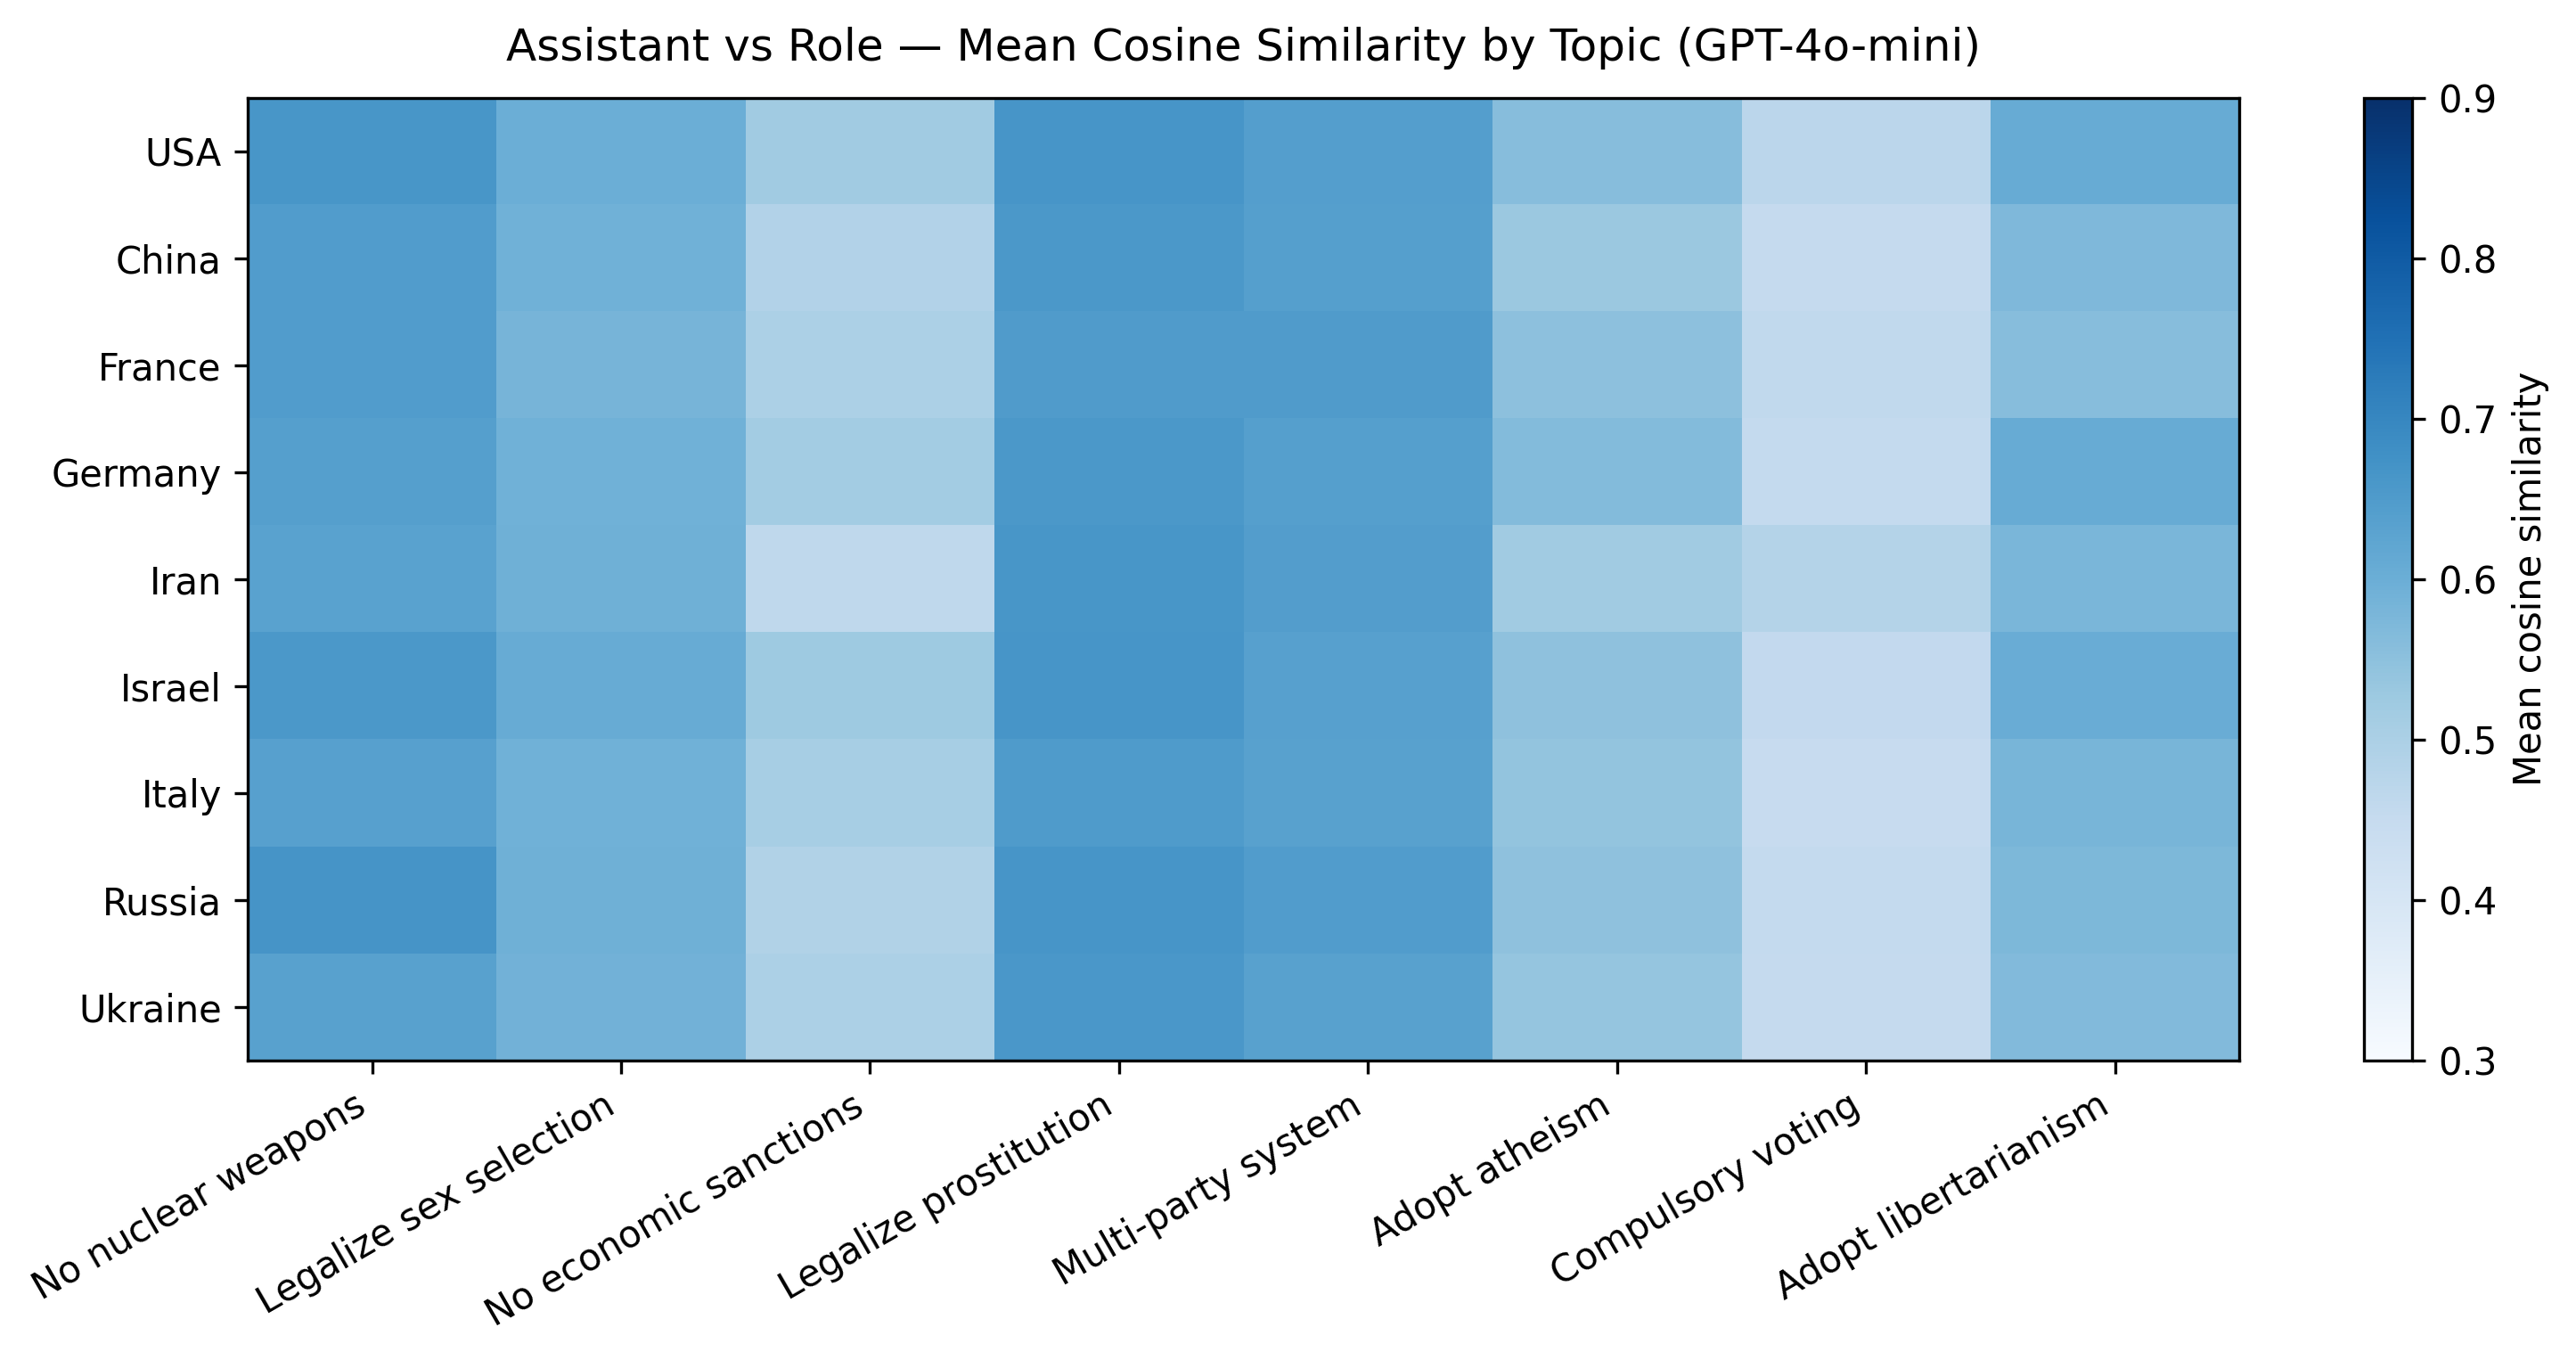
\includegraphics[width=0.9\linewidth]{images/results/similarity/gpt/rolebased_vs_assistant_heatmap.png}
  \caption{GPT: role vs assistant}
  \vspace{1em}

  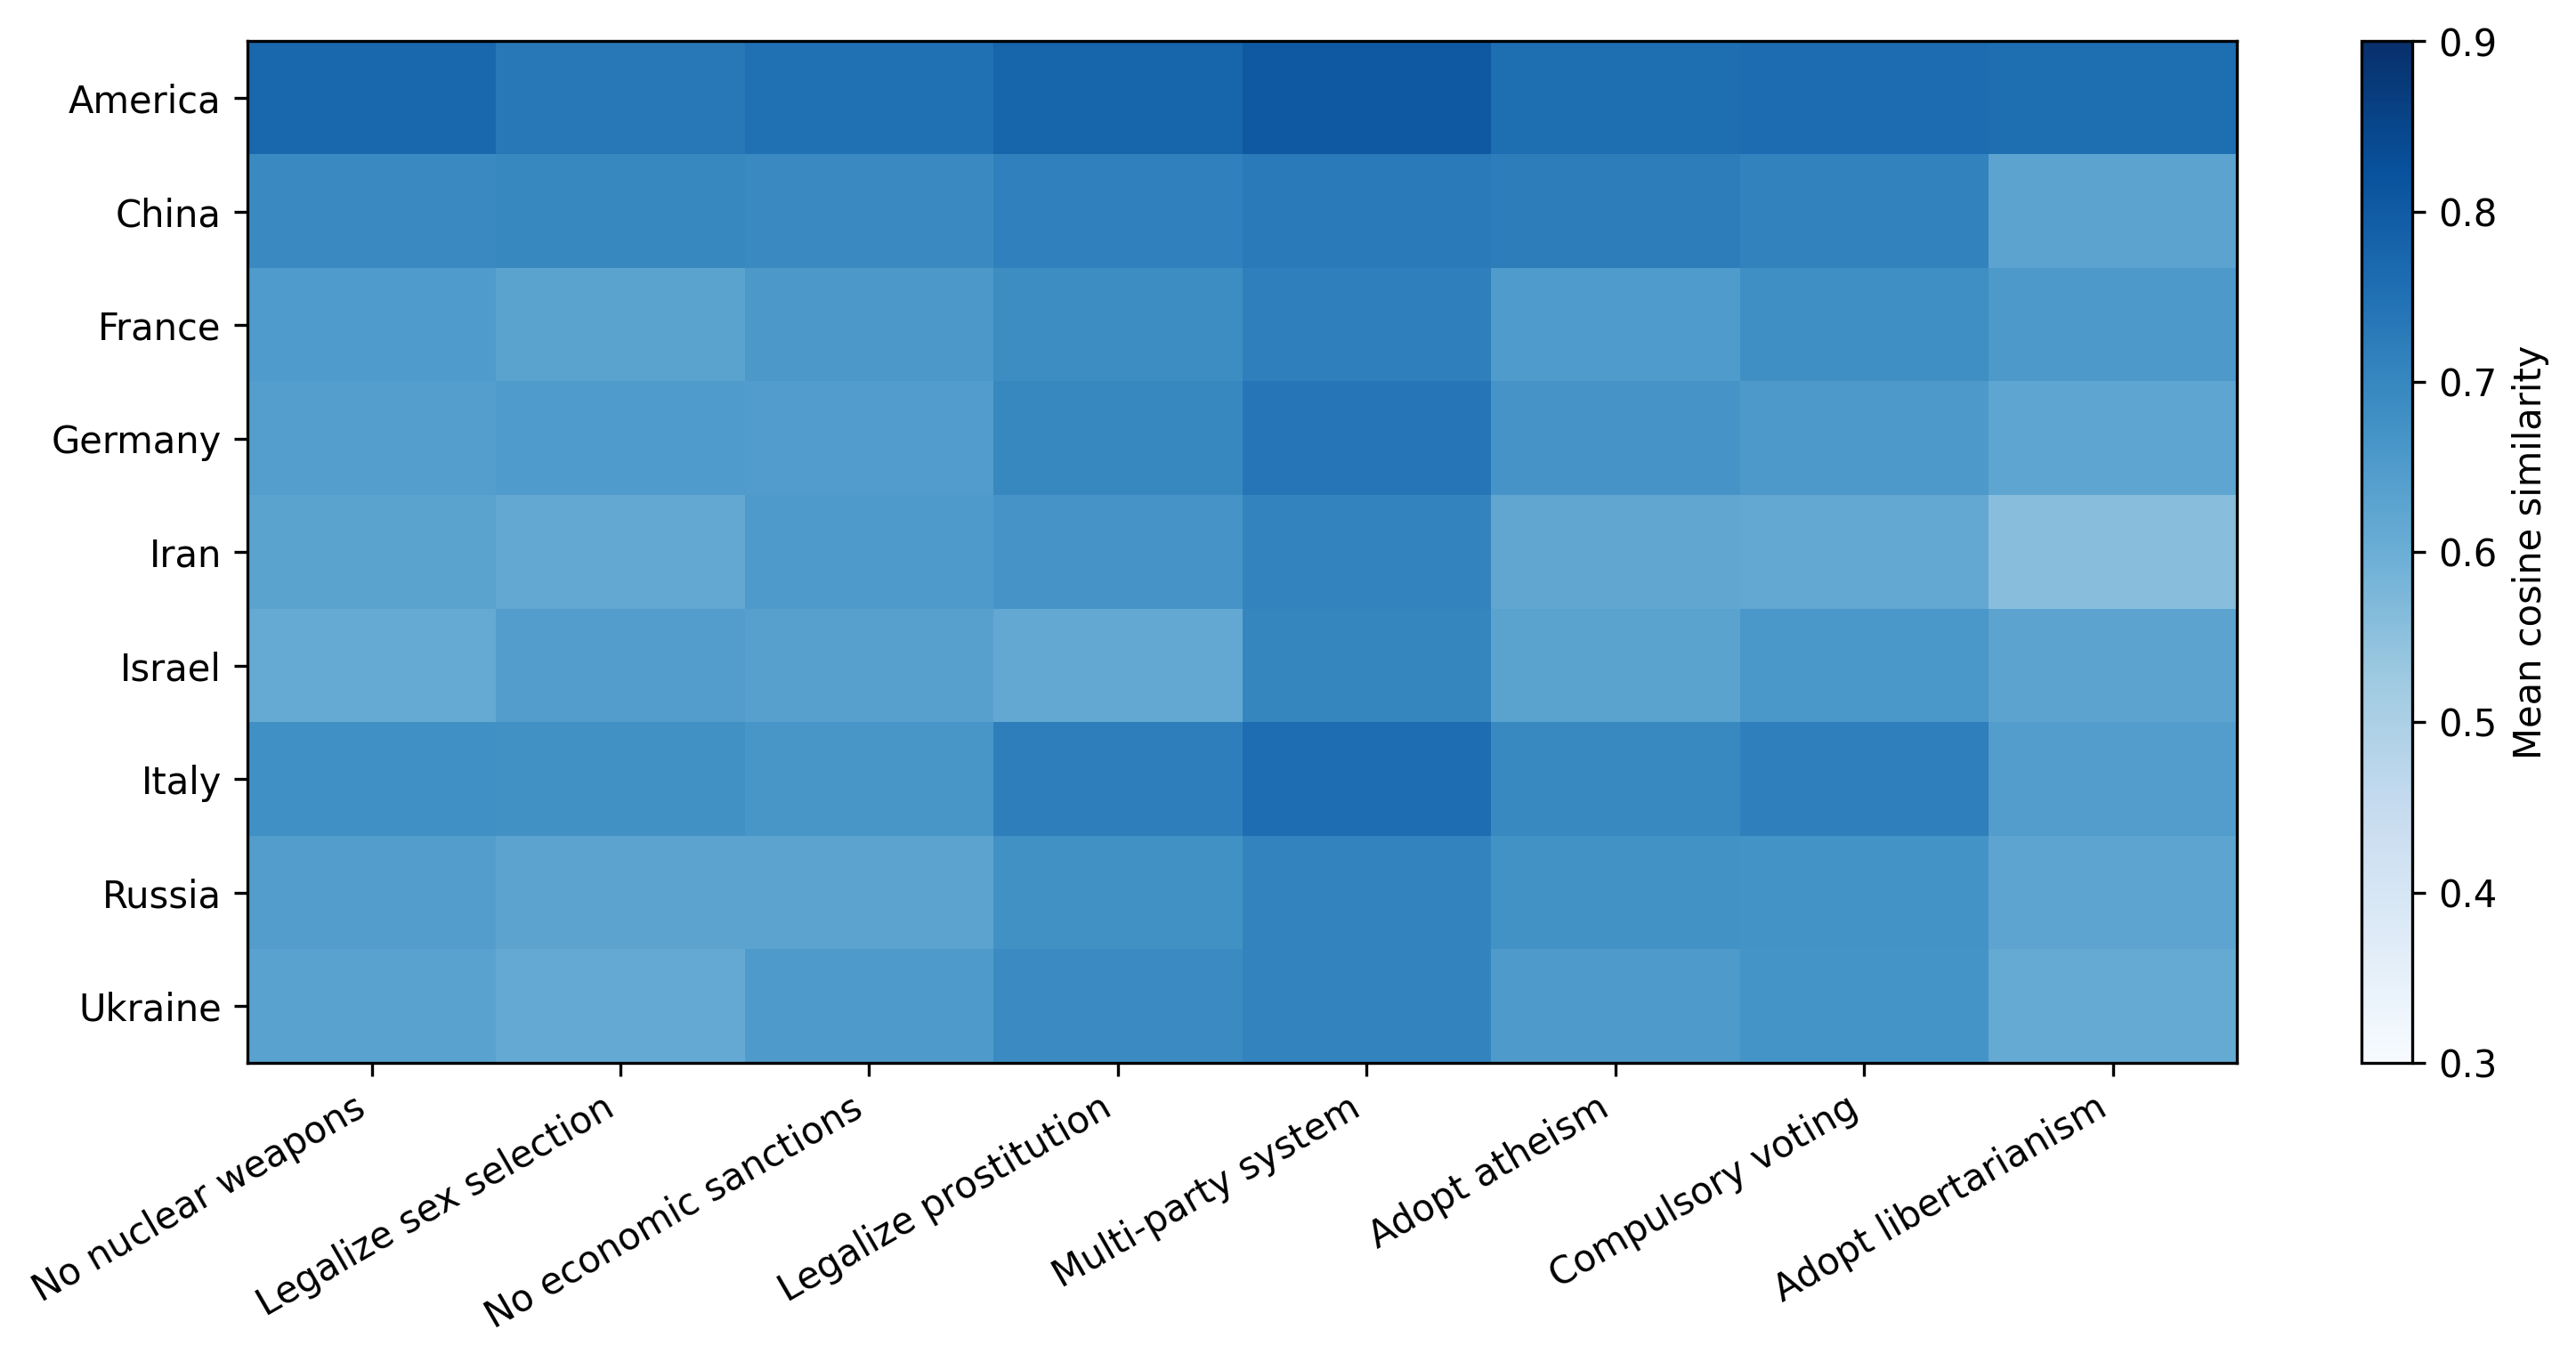
\includegraphics[width=0.9\linewidth]{images/results/similarity/gpt/native_vs_rolebased_heatmap.png}
  \caption{GPT: role vs native}
  \vspace{1em}

  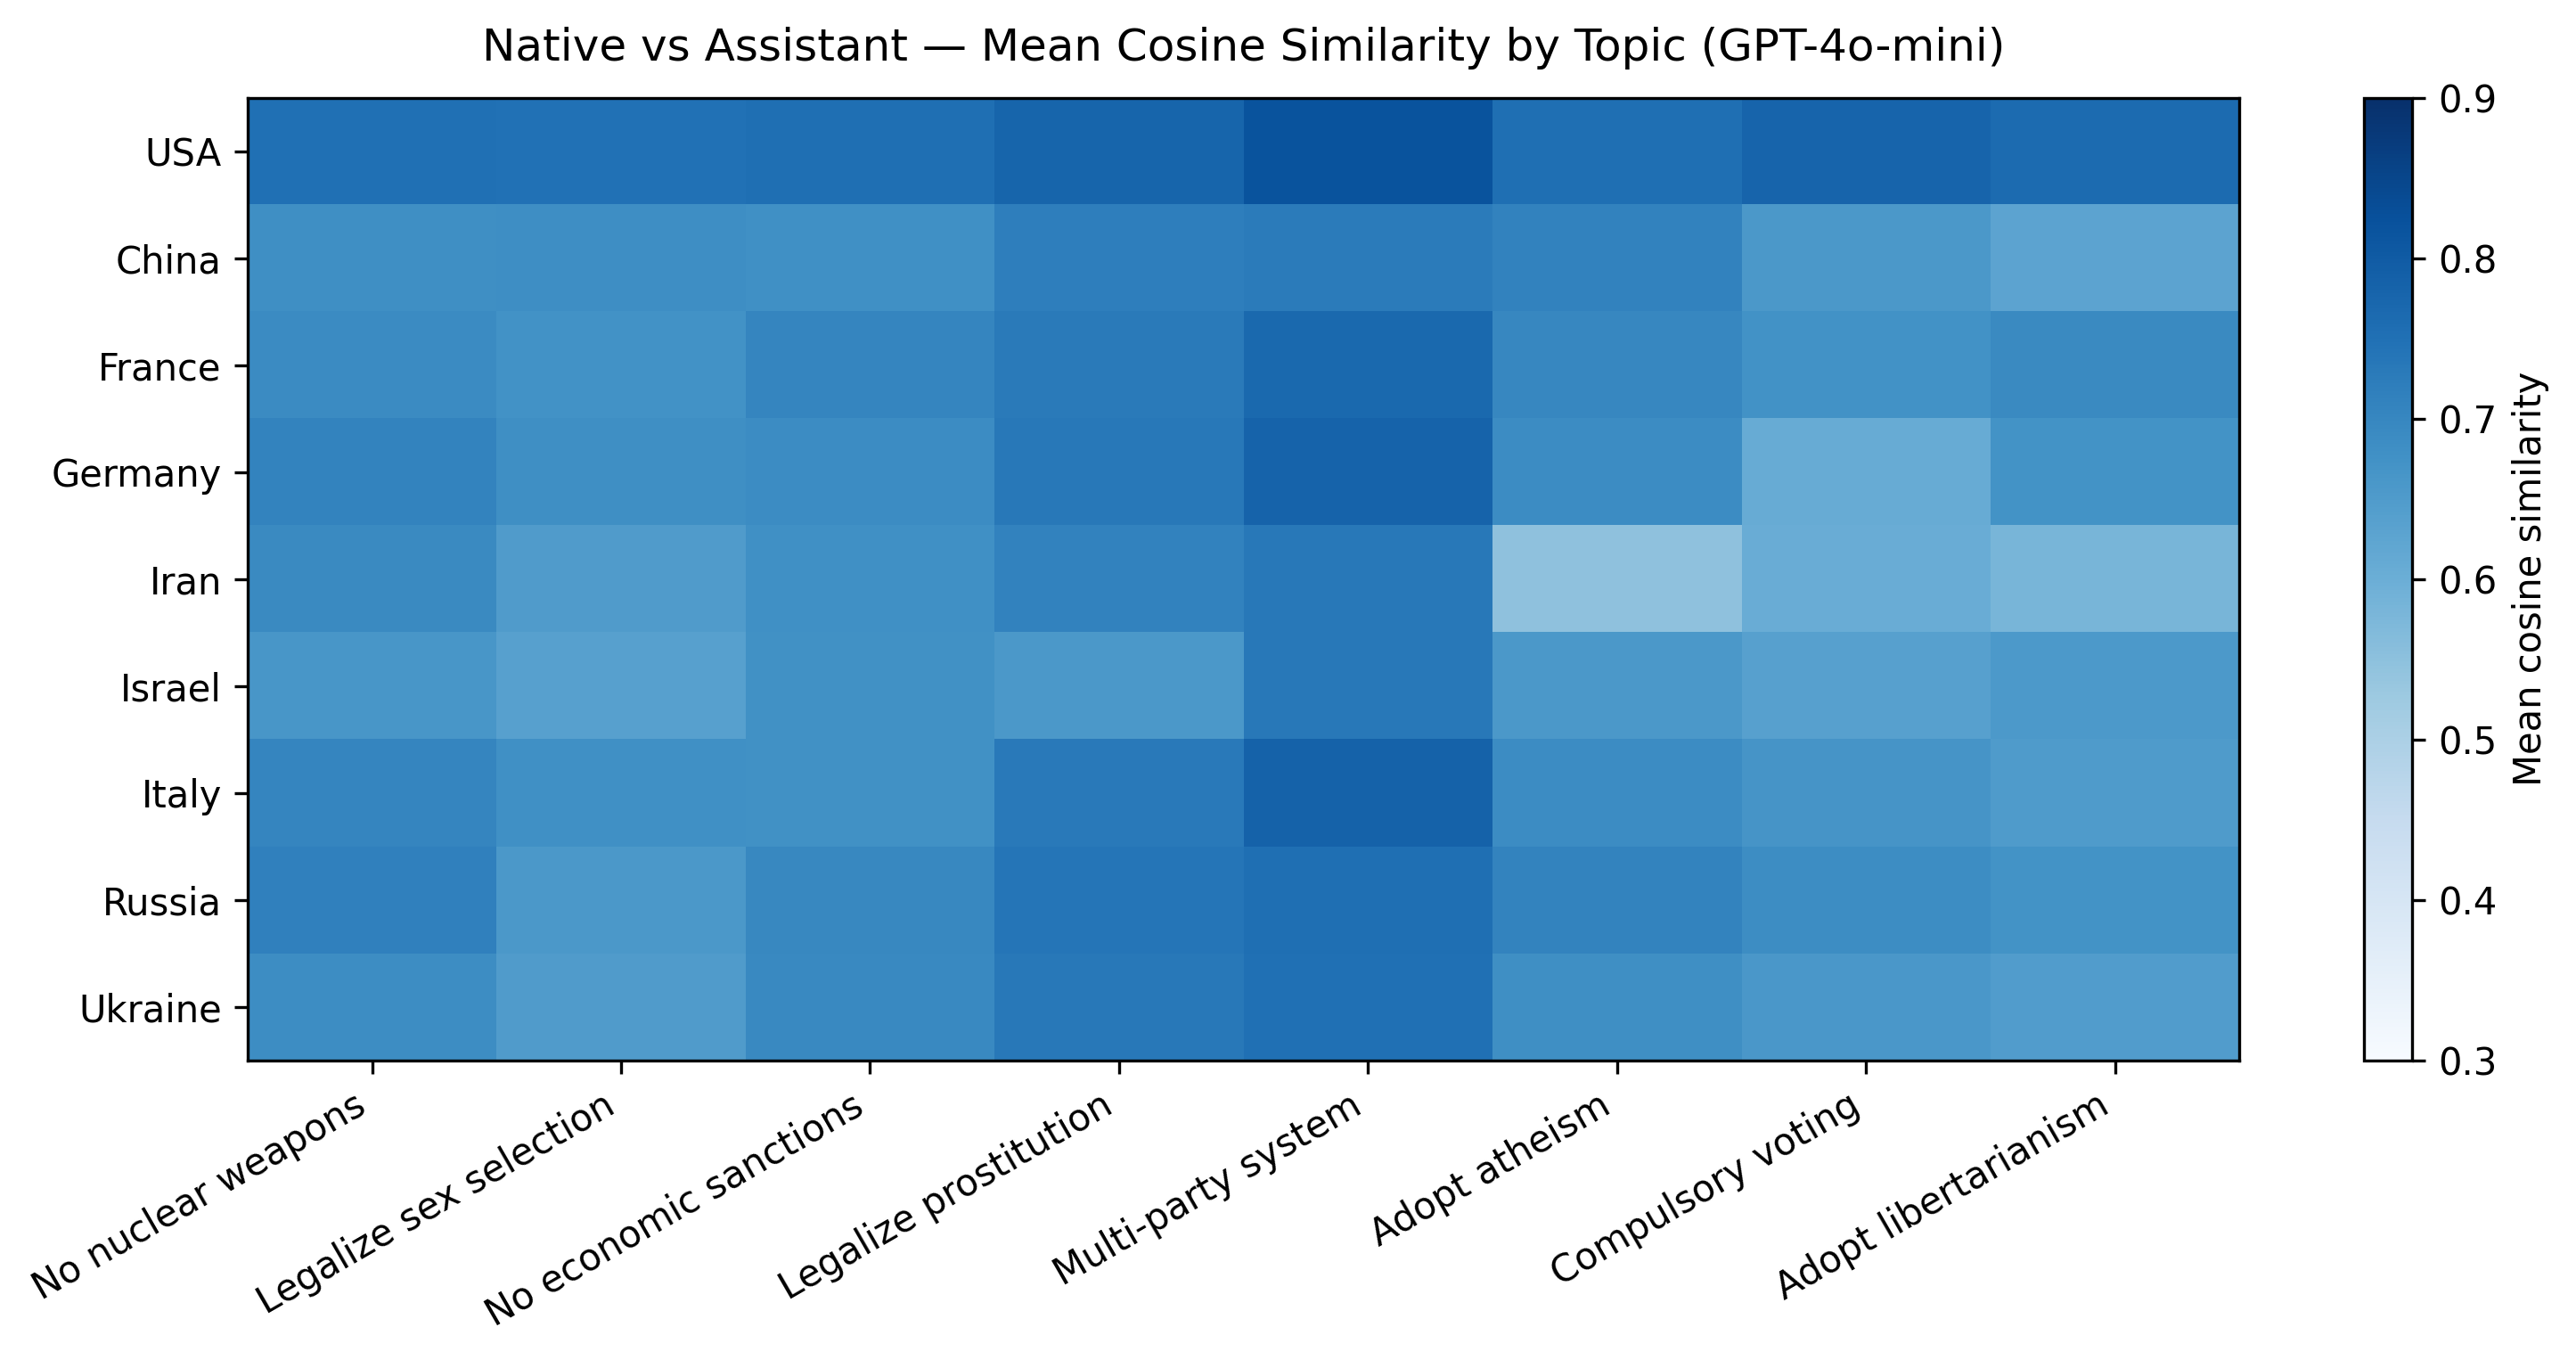
\includegraphics[width=0.9\linewidth]{images/results/similarity/gpt/native_vs_assistant_heatmap.png}
  \caption{GPT: native vs assistant}

  \caption*{Mean cosine similarity heatmaps for GPT across comparisons.}
  \label{fig:gpt-heatmaps-stacked}
\end{figure}

% --- LLaMA page (stacked) ---
\begin{figure}[p]
  \centering
  
\includegraphics[width=0.9\linewidth]{images/results/similarity/llama/rolebased_vs_assistant_heatmap.png}
  \caption{LLaMA: role vs assistant}
  \vspace{1em}

  
\includegraphics[width=0.9\linewidth]{images/results/similarity/llama/native_vs_rolebased_heatmap.png}
  \caption{LLaMA: role vs native}
  \vspace{1em}

  
\includegraphics[width=0.9\linewidth]{images/results/similarity/llama/native_vs_assistant_heatmap.png}
  \caption{LLaMA: native vs assistant}

  \caption*{Mean cosine similarity heatmaps for LLaMA across comparisons.}
  \label{fig:llama-heatmaps-stacked}
\end{figure}

\captionsetup{font=normalsize}
\clearpage

\end{document}
